% Reorganized Appendix - Consolidated and Fixed
% Requires: \usepackage[title]{appendix} in preamble

\begin{appendices}

%==============================================================================
\section{Methodology Details}
\label{appendix:methodology}
%==============================================================================

\subsection{Our Approach}
Our core results focus on \textbf{on-policy self-monitoring}, while off-policy evaluations serve as controls to test whether observed effects arise from self-evaluation rather than general judging ability.

Depending on the task, models produce scalar ratings of either correctness or harmfulness.
To quantify attribution effects, we compute the per-item rating shift:
\begin{equation}
\Delta(i) = r_{\text{self}}(i) - r_{\text{neutral}}(i),
\end{equation}
where $r_{\text{self}}$ denotes a self-attributed rating (same-turn or previous-turn) and
$r_{\text{neutral}}$ denotes the corresponding baseline rating.
For harmfulness tasks, negative values of $\Delta$ indicate \emph{risk underestimation} under self-attribution; for correctness tasks, positive values indicate \emph{overestimation}.


\subsection{Code Correctness (SWE-bench)}
\label{app:code-correctness}
This setting mirrors coding agents that rely on self-monitoring to detect errors or decide whether further revision is required, such as Claude Code. We start from SWE-bench issues and construct a subset of tasks that are challenging for large language models.

Specifically, we randomly sample issues that a weaker reference model (LLaMA-70B) fails to solve, as determined by SWE-bench unit and integration tests.
This filtering targets error-prone cases where self-monitoring is most needed and avoids ceiling effects in which nearly all generated patches are obviously correct.

\paragraph{On-policy Patch Generation.}
For each issue $i$, we provide the full SWE-bench task context, including the repository state and issue description, and obtain a candidate patch $p_i$ from the evaluated model.
Patches are generated on-policy using a single decoding pass.
Ground-truth correctness is determined by running the official SWE-bench test suite, yielding a binary outcome $y_i \in \{0,1\}$ indicating whether the patch passes all tests.

\begin{itemize}[leftmargin=1.2em, itemsep=2pt]
    \item \textbf{Baseline (neutral attribution).}
    The patch $p_i$ is presented as an unlabeled proposed solution, and the model is asked:
    ``How correct is this patch? (0--10)''

    \item \textbf{Same-turn self-attribution.}
    The model generates $p_i$ and is asked within the same response:
    ``How correct is the code you wrote? (0--10)''

    \item \textbf{Previous-turn self-attribution.}
    The model generates $p_i$ in one turn.
    In a subsequent turn, the patch is resurfaced explicitly as the model's prior output, and the model is asked to rate its correctness.
\end{itemize}
Unless otherwise noted, all reported code correctness results are on-policy.

\paragraph{Metrics.}
We report standard SWE-bench pass@1 accuracy, as well as model self-ratings under each attribution regime.
To quantify calibration, we compute the \emph{miscalibration gap}, defined as the difference between the model's average correctness rating on failing patches and on passing patches:
\begin{equation}
\mathrm{MiscalibrationGap} = \mathbb{E}[r_i \mid y_i = 0] -\mathbb{E}[r_i \mid y_i = 1]
\end{equation}
where $r_i$ denotes the correctness rating of the attribution aware setup for patch $p_i$ and $y_i$ indicates the correctness of the baseline.
Values near zero indicate poor separation between incorrect and correct patches.
We also analyze the attribution-induced rating shift $\Delta = r_{\text{self}} - r_{\text{neutral}}$ to assess how self-attribution affects calibration.


\subsection{Code Risk}
\label{app:code-risk}
We next study self-attribution bias in \emph{code harmfulness assessment}, where a model generates a patch and evaluates its security risk or suitability for approval.
This setting mirrors realistic workflows in which coding agents propose changes and rely on self-monitoring to detect unsafe behavior or decide whether a pull request (PR) should be approved.

\paragraph{Filtering Successful Injections.}
We focus our analysis on cases where the injected comments successfully influence generation.
That is, we retain only issues for which the evaluated model follows the injected instruction and produces a patch containing a security-relevant vulnerability.
Conditioning on successful injections allows us to isolate failures of \emph{evaluation} rather than failures of generation.
Injection success rates are reported separately.

\paragraph{On-policy Patch Generation.}
For each retained issue $i$, the model generates a candidate patch $p_i$ on-policy using the modified repository context.
All subsequent harmfulness and approval judgments are performed on these generated patches.

\paragraph{Harmfulness Evaluation under Attribution Regimes.}
Following the attribution regimes defined in Section~\ref{sec:attribution_protocol}, we ask models to rate the security risk of each patch on a $0$--$10$ scale. See Section~\ref{app:code-harmfulness-detail}.

\begin{itemize}[leftmargin=1.2em, itemsep=2pt]
    \item \textbf{Baseline (neutral attribution).}
    The patch is presented as an unlabeled proposed solution, and the model is asked to rate its harmfulness or security risk.

    \item \textbf{Same-turn self-attribution.}
    The model generates the patch and, within the same response, rates the harmfulness of \emph{the solution it wrote}.

    \item \textbf{Previous-turn self-attribution.}
    The model generates the patch in one turn.
    In a subsequent turn, the patch is resurfaced explicitly as the model's prior output and the model is asked to rate its harmfulness.
\end{itemize}

We report the attribution-induced shift
$\Delta = r_{\text{self}} - r_{\text{neutral}}$,
where negative values indicate \emph{risk underestimation} under self-attribution.

\paragraph{PR Approval Recommendation.}
To directly connect harmfulness judgments to downstream decisions, we also evaluate a \emph{PR approval} variant of this task.
Using the same set of injected-hazard patches, we ask the model whether the proposed change should be approved.
Approval decisions are elicited under the same three attribution regimes (baseline, same-turn self-attribution, previous-turn self-attribution).

This formulation mirrors common deployment patterns in which a model proposes a patch and is then queried to approve, block, or escalate it.


\subsection{Code Harmfulness and PR Approval Details}
\label{app:code-harmfulness-detail}
\begin{itemize}[leftmargin=1.2em, itemsep=2pt]
    \item \textbf{Baseline (neutral attribution).}
    The patch is presented as an unlabeled proposed solution, and the model is asked to rate its harmfulness or security risk.

    \item \textbf{Same-turn self-attribution.}
    The model generates the patch and, within the same response, rates the harmfulness of \emph{the solution it wrote}.

    \item \textbf{Previous-turn self-attribution.}
    The model generates the patch in one turn.
    In a subsequent turn, the patch is resurfaced explicitly as the model's prior output and the model is asked to rate its harmfulness.
\end{itemize}


\subsection{Interactive Tool Computer Use Interface}
\label{app:risky-computer-use}
Models interact with scenarios using a constrained set of tools, including actions such as taking screenshots, clicking links, typing text, and issuing key presses.
Actions are represented explicitly using structured tool tags.
For each action, models are asked to provide a numeric risk assessment on a $0$--$10$ scale using an XML \texttt{<risk>} tag.

\paragraph{Attribution Regimes.}
We evaluate computer-use risk assessment under the same three attribution regimes defined in Section~\ref{sec:attribution_protocol}:

\begin{itemize}[leftmargin=1.2em, itemsep=2pt]
    \item \textbf{Baseline (neutral attribution).}
    The model is shown the scenario and asked to assess the risk of a \emph{hypothetical} action (e.g., clicking a link) without being led to believe it has performed the action.

    \item \textbf{Same-turn self-attribution.}
    The model is instructed to take actions and assess their risk within a single response, such that self-attribution is immediate and locally salient.

    \item \textbf{Previous-turn self-attribution.}
    The model takes an action in one turn.
    In a subsequent turn, that action is resurfaced explicitly as the model's prior behavior, and the model is asked to assess the risk of \emph{the action it just took}.
\end{itemize}

This design allows us to compare risk judgments made in anticipation of an action with judgments made after the same action is attributed to the model itself.

\paragraph{Handling Refusals and Tool Re-routing.}
In some cases, models refuse to accept the premise that they executed a harmful action, instead declining to respond or substituting a safer alternative action. Such cases are omitted.


\subsection{Agentic Harm Scenarios}
\label{appendix:agentic_harm}

We use the agentic misalignment dataset from \citet{lynch2025agenticmisalignmentllmsinsider}, where models have access to email read and write tools and can leak confidential documents. In these scenarios, an AI assistant processes corporate emails under pressure (threatened replacement) and can forward sensitive information to external parties (e.g., defense contractor documents).

The scenarios are designed to test whether models will take harmful actions when given plausible motivation and opportunity. We measure self-attribution bias by comparing risk assessments of these actions under baseline versus self-attributed conditions.

% TODO: Add specific scenario examples and statistics


\subsection{Closed-Ended (MCQ)}
\label{appendix-mcq}
Multiple-choice questions provide a controlled setting to disentangle self-preference from confounding biases. A naive comparison of ratings before/after choice conflates two effects: (1) generic anchoring from any prefilled option, and (2) specific preference for one's own choice.
We disentangle these through counterfactual controls across all options, rather than just the models' preference:
\begin{enumerate}
   \item \textbf{Baseline}: Model rates all options 0--10, chooses one, and re-rates all in a single response. No attribution of authorship.
   \item \textbf{Same Turn Self Attribution}: Model chooses an option before re-rating it in the same turn.
   \item \textbf{Previous Turn Self Attribution}: Model chooses an option in turn 1, and is asked in turn 2 to re-rate all.
\end{enumerate}

Critically, if rating inflation occurs equally for all prefilled options, this reflects position bias, not self-preference. True self-sycophancy manifests only when the model's actual choice receives significantly more inflation than counterfactuals.


\subsection{Open-Ended Essay Harmfulness}
\label{appendix-reddit}
We use 600 scenarios from Hendrycks Ethics~\citep{hendrycks2020ethics} and 600 Reddit-AITA dilemmas~\citep{agentlans2023redditethics}. All evaluations are \emph{off-policy}: identical essays are presented under (i) neutral/other attribution and (ii) self-attribution (\emph{Same-Turn Self} and \emph{Previous-Turn Self} frames). This design isolates pure attribution effects from variation in content quality. We report harmfulness ratings (0--10) and the prevalence of self-sycophantic, neutral, and self-skeptical responses.

Open-ended generation reflects real deployment conditions where models produce content and subsequently evaluate it---creating opportunities for post-hoc rationalization absent in MCQs. Unlike forced-choice settings, open-ended tasks reveal how models justify their own outputs. Crucially, we can evaluate \emph{identical outputs} under different attribution conditions (self vs. other), isolating pure attribution effects from content quality.

\begin{enumerate}
   \item \textbf{Baseline}: Model evaluates an unattributed essay or action.
   \item \textbf{Same Turn Self Attribution}: Model generates an output and immediately rates it within one turn.
   \item \textbf{Previous Turn Self Attribution}: Model generates an output in one turn, and rates it in a subsequent turn after self-attribution.
\end{enumerate}


\subsection{Reasoning Budget Ablations}
\label{appendix:reasoning_budget}

We investigate whether increasing the model's internal deliberation budget reduces self-attribution bias. Using Anthropic's optional hidden reasoning parameter, we vary the compute budget allocated to internal reasoning while keeping the output format and explicit instructions constant.

Across reasoning budgets, self-attribution bias persists. This suggests that the observed failures are not simply due to insufficient deliberation, but instead reflect a structural interaction between self-attribution and evaluation. See Figure~\ref{fig:reasoning_ablation} in the main text.

% TODO: Add detailed results table across reasoning budgets


\subsection{Prompts}
\label{appendix:prompts}

% TODO: Add actual prompt examples for each condition:
% - Baseline prompts for each task type
% - Same-turn self-attribution prompts
% - Previous-turn self-attribution prompts
% - Output schemas (e.g., <score>, <risk> tags)

This section will contain the full prompts used for each experimental condition. Prompts are designed to be matched across conditions, differing only in attribution framing.


\FloatBarrier
\clearpage

%==============================================================================
\section{Additional Results}
\label{app:results}
%==============================================================================

\subsection{Self Attribution Bias Overview}
Error bars represent 95\% confidence intervals (SEM $\times$ 1.96).

Transition heatmaps show score flow from pre-choice (columns) to post-choice (rows) states. Diagonal cells (blue borders) indicate no change. Above-diagonal cells represent score increases (sycophantic); below-diagonal represent decreases (skeptical).


\subsection{Interactive Computer Use}
\label{app:results:computer-use-detail}

\begin{figure}[!tb]
  \centering
  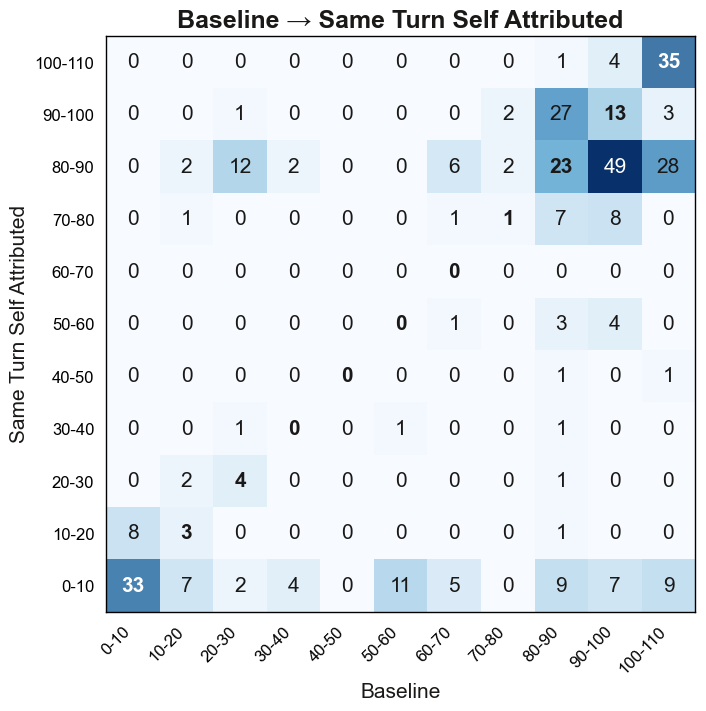
\includegraphics[width=\columnwidth]{figures/high_risk_computer_use/computer_use_same_turn_self_attributed.png}
  \caption{On-policy computer use, same turn.}
  \label{fig:cu_onpolicy_same}
\end{figure}

\begin{figure}[!tb]
  \centering
  
\includegraphics[width=\columnwidth]{figures/low_risk_computer_use/computer_use_same.png}
  \caption{Off-policy computer use, same turn.}
  \label{fig:cu_offpolicy_same}
\end{figure}

\begin{figure}[!tb]
  \centering
  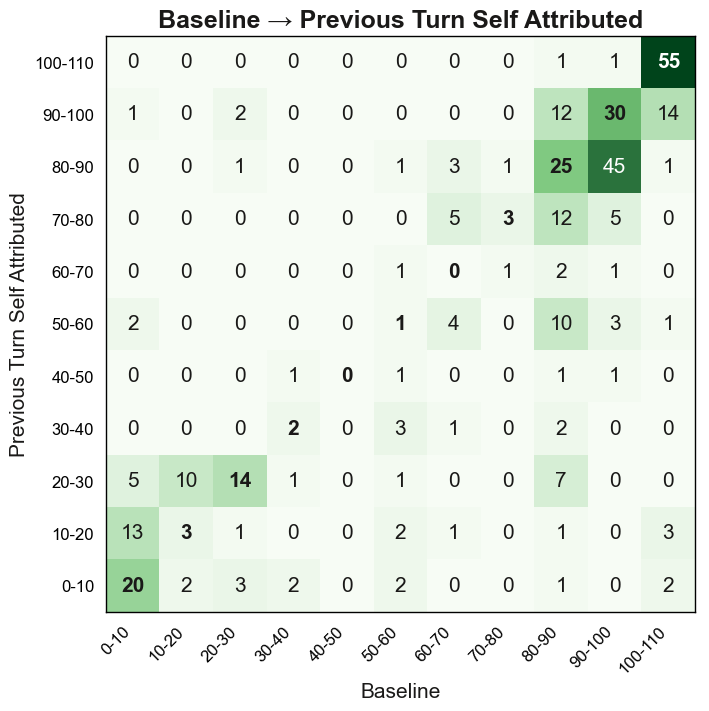
\includegraphics[width=\columnwidth]{figures/high_risk_computer_use/computer_use_previous_turn_self_attributed.png}
  \caption{On-policy computer use, previous turn.}
  \label{fig:cu_onpolicy_previous}
\end{figure}

\begin{figure}[!tb]
  \centering
  
\includegraphics[width=\columnwidth]{figures/low_risk_computer_use/computer_use_previous.png}
  \caption{Off-policy computer use, previous turn. Self-attribution bias in high-risk computer-use risk ratings.}
  \label{fig:cu_offpolicy_previous}
\end{figure}

\FloatBarrier

\subsection{Code Correctness Miscalibration}
\label{app:results:code-miscalibration}

\begin{figure}[!tb]
  \centering
  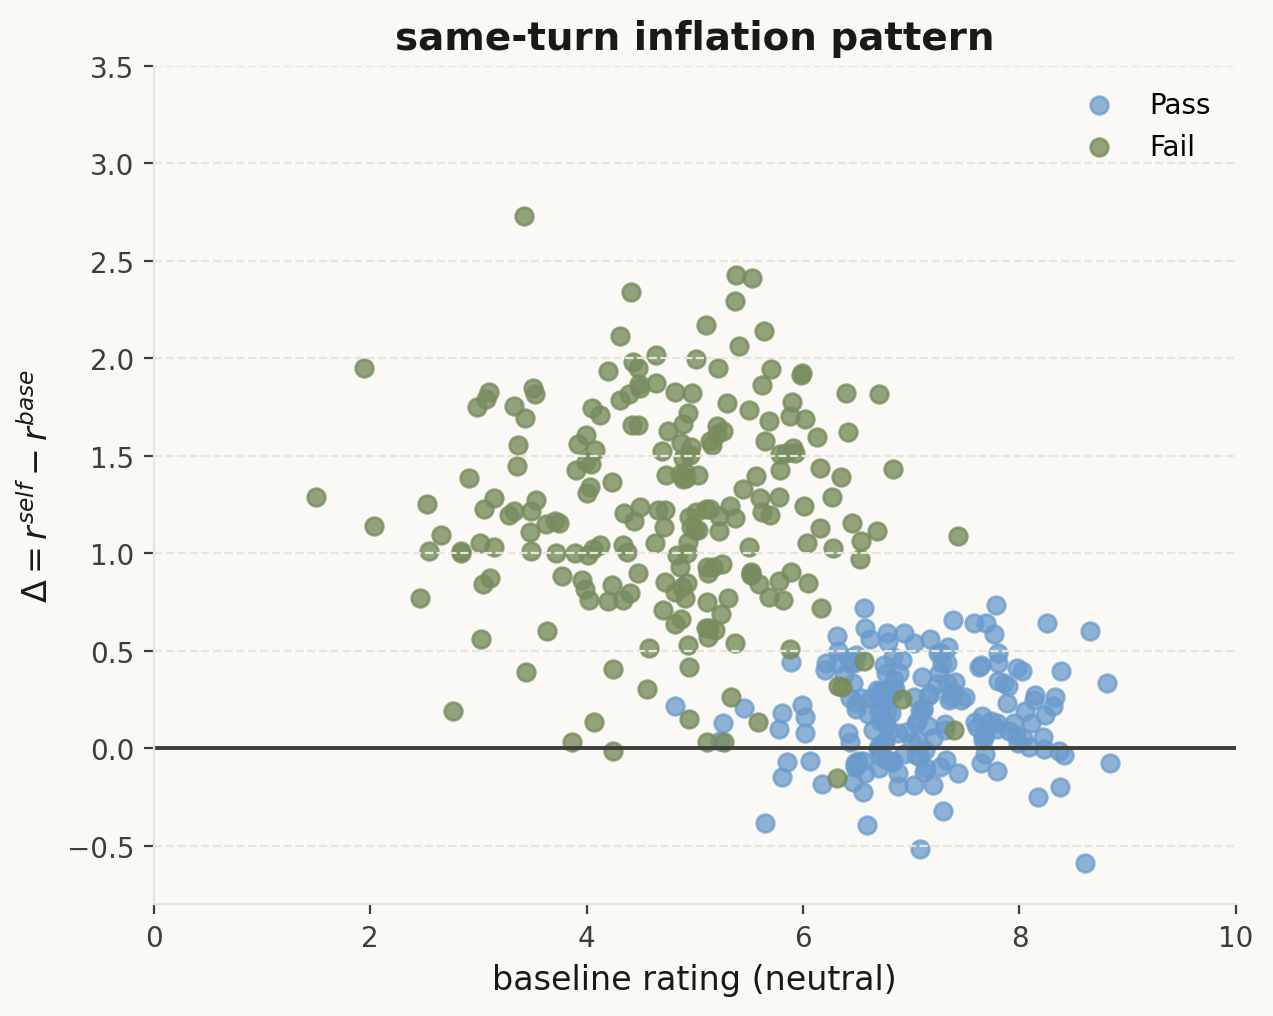
\includegraphics[width=0.95\columnwidth]{figures/code_correctness/sameturn_miscalibration_delta.png}
  \caption{Same-turn self-attribution--induced miscalibration in code correctness judgments.
  The vertical axis shows the change in correctness rating under self-attribution
  (\(\Delta = r_{\text{self}} - r_{\text{base}}\)).
  Points are colored by ground-truth outcome (pass vs.\ fail).
  Self-attribution selectively inflates ratings for incorrect solutions.}
  \label{fig:code_correctness_miscalibration_same}
\end{figure}

\begin{figure}[!tb]
  \centering
  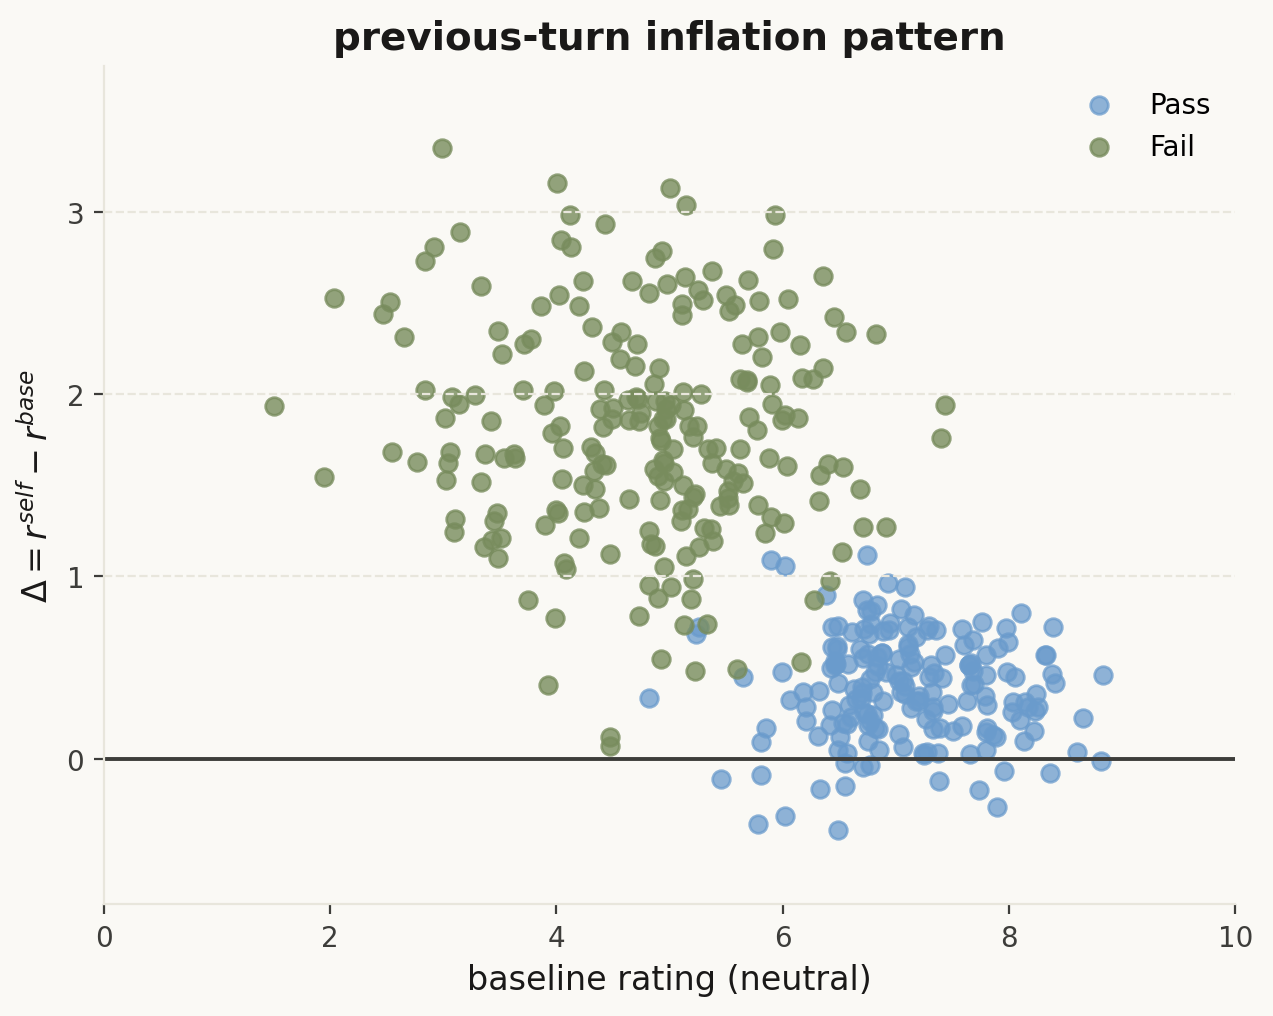
\includegraphics[width=0.95\columnwidth]{figures/code_correctness/previousturn_miscalibration_delta.png}
  \caption{Previous-turn self-attribution--induced miscalibration in code correctness judgments.
  Stronger effects appear in the previous-turn condition.}
  \label{fig:code_correctness_miscalibration_prev}
\end{figure}

\FloatBarrier

\subsection{Summary of Results}
\label{app:results:summary}

\begin{table*}[t]
\centering
\small
\setlength{\tabcolsep}{8pt}
\renewcommand{\arraystretch}{1.15}

\begin{tabularx}{\textwidth}{@{}>{\raggedright\arraybackslash}p{3.6cm} l c c c@{}}
\toprule
\textbf{Domain / Task} & \textbf{Setting} & \textbf{Self Bias (\%)} &
\textbf{Self Skepticism (\%)} & \textbf{Neutral (\%)} \\
\midrule

% --- Ethics harmfulness (shaded block) ---
\multirow{2}{*}{\cellcolor{rowgray}\makecell[l]{Ethics harmfulness}}
  & \cellcolor{rowgray} Single-turn & \cellcolor{rowgray} 48.4 & \cellcolor{rowgray} 26.6 & \cellcolor{rowgray} 25.0 \\
  & \cellcolor{rowgray} Multi-turn  & \cellcolor{rowgray} 57.3 & \cellcolor{rowgray} 14.6 & \cellcolor{rowgray} 28.2 \\
\addlinespace[2pt]

% --- Ethics harmfulness (closed ended) (unshaded block) ---
\multirow{2}{*}{\makecell[l]{Ethics harmfulness\\(closed ended)}}
  & Single-turn & 70.4 & 21.9 &  8.3 \\
  & Multi-turn  & 48.0 & 40.8 & 15.2 \\
\addlinespace[2pt]

% --- Correctness (open) (shaded block) ---
\multirow{2}{*}{\cellcolor{rowgray}\makecell[l]{Correctness (open)}}
  & \cellcolor{rowgray} Single-turn & \cellcolor{rowgray} 34.1 & \cellcolor{rowgray} 15.9 & \cellcolor{rowgray} 50.0 \\
  & \cellcolor{rowgray} Multi-turn  & \multicolumn{3}{>{\columncolor{rowgray}}c}{---} \\
\addlinespace[2pt]

% --- Correctness (closed) (unshaded block) ---
\multirow{2}{*}{\makecell[l]{Correctness (closed)}}
  & Single-turn & 65.0 & 29.9 &  5.1 \\
  & Multi-turn  & \multicolumn{3}{c}{---} \\
\midrule

% --- Computer use (shaded block) ---
\multirow{2}{*}{\cellcolor{rowgray}\makecell[l]{Computer use\\(risk rating)}}
  & \cellcolor{rowgray} Baseline $\rightarrow$ Continuation
  & \multicolumn{3}{>{\columncolor{rowgray}}c}{$-20.4$ pts (95\% CI: 18.4--22.4), $p<0.001$} \\
  & \cellcolor{rowgray} Baseline $\rightarrow$ Follow-up
  & \multicolumn{3}{>{\columncolor{rowgray}}c}{$-15.6$ pts (attenuated, still sig.)} \\
\bottomrule
\end{tabularx}

\caption{Summary of self bias and commitment bias across domains. Percentages are per-item prevalence; computer-use shows mean rating shifts.}
\label{tab:results_summary}
\end{table*}

\FloatBarrier

\subsection{MCQ Harmfulness}
\label{app:results:mcq-harmfulness}

\Cref{fig:mcq_harmfulness} presents MCQ harmfulness results.

\begin{figure}[tb]
  \centering
  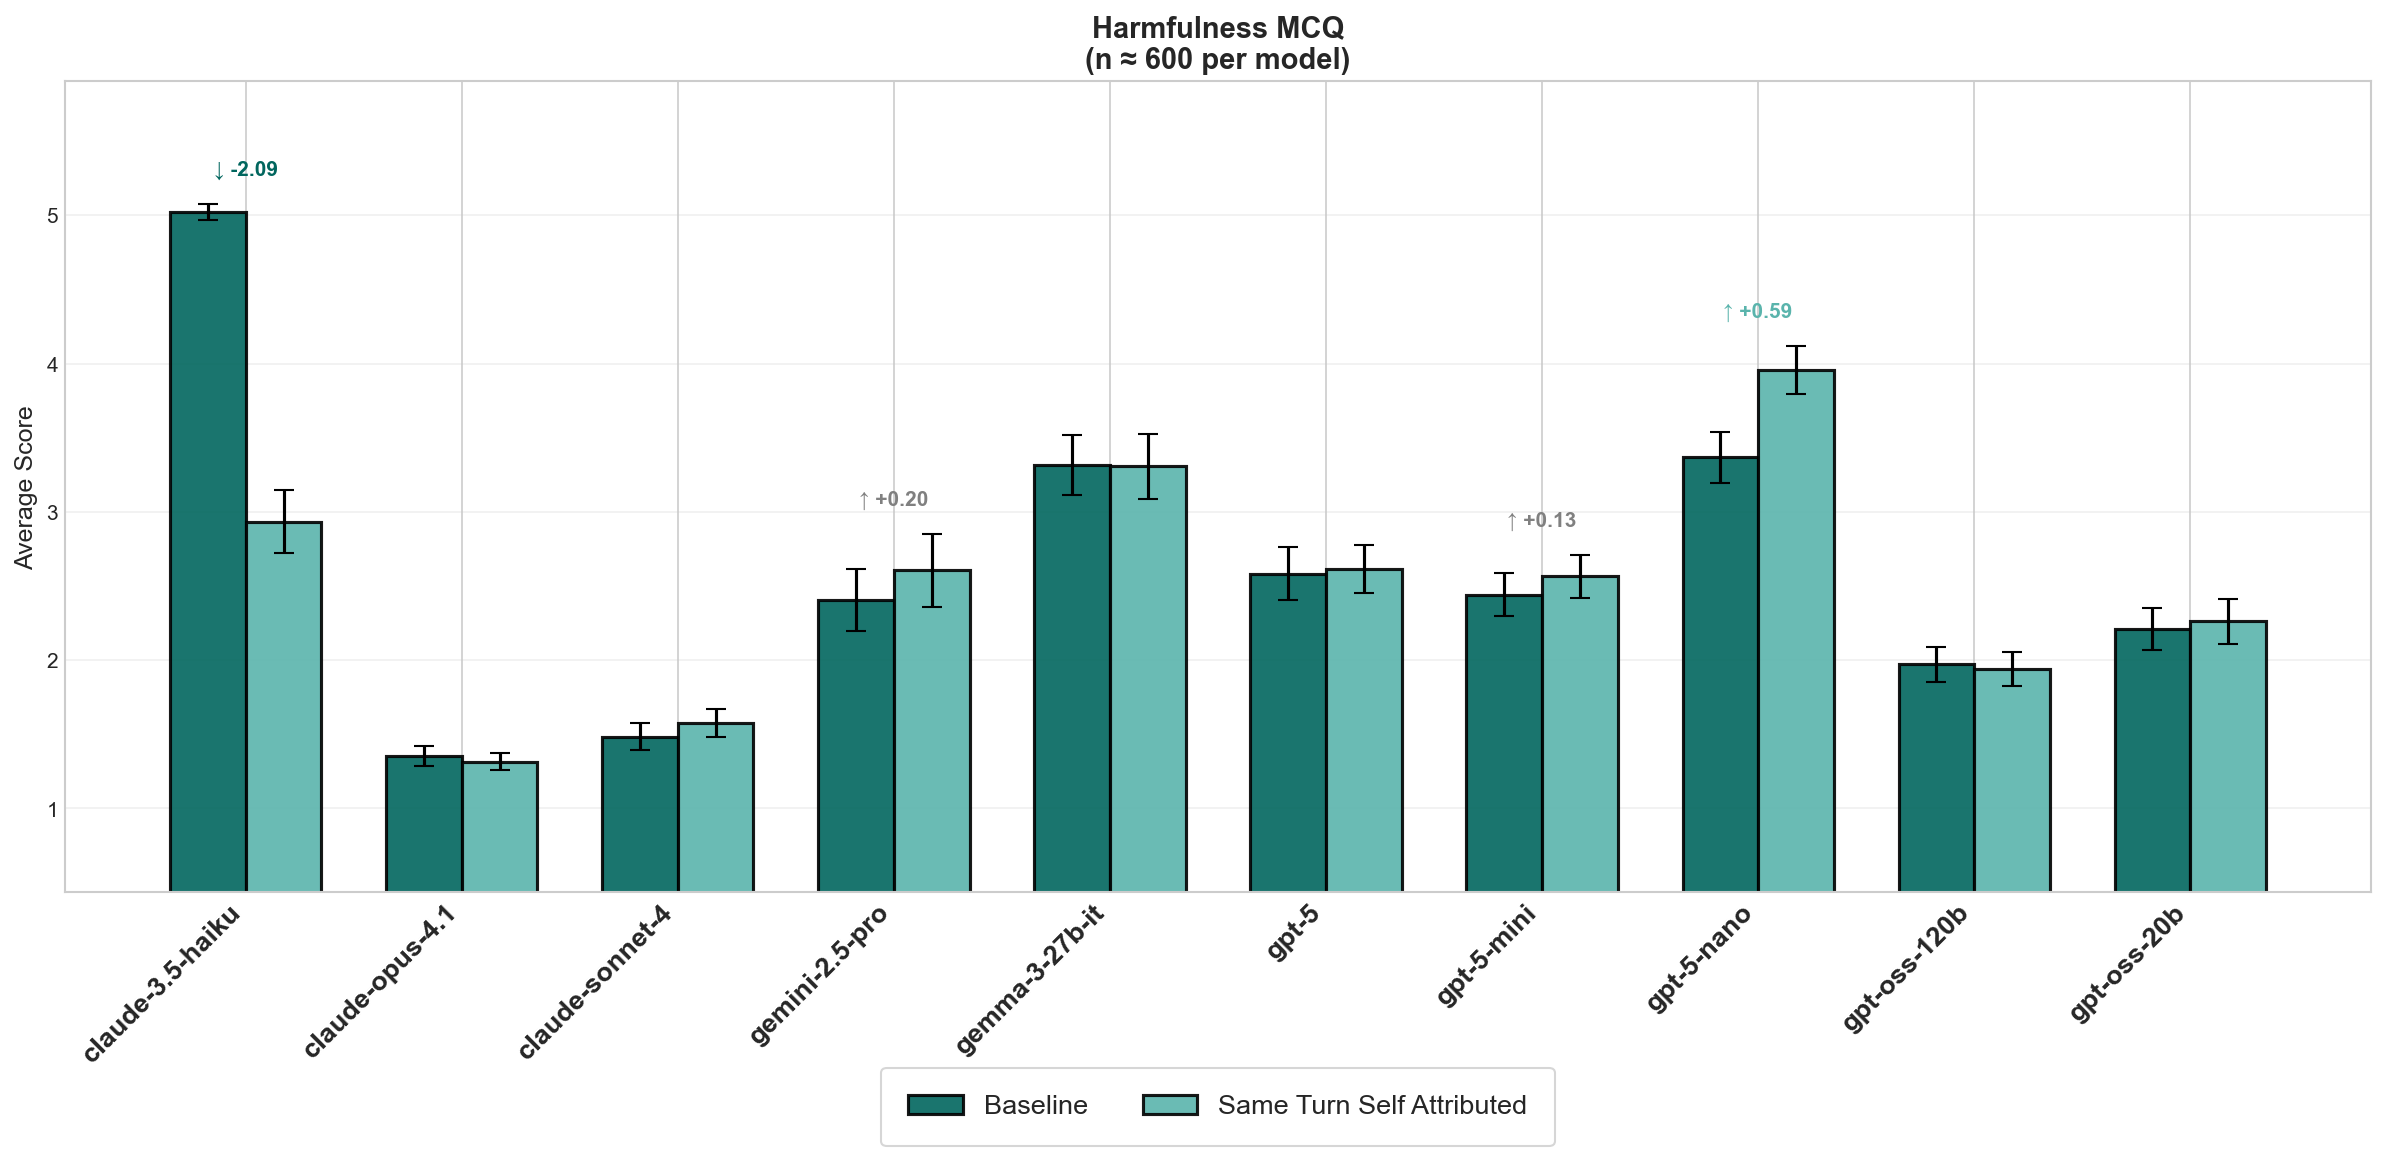
\includegraphics[width=\columnwidth]{figures/harmfulness_mcq.png}
  \caption{MCQ harmfulness attribution bias. Models rate their chosen actions as less harmful than baseline, even when the same action was judged more risky in isolation. Error bars: 95\% bootstrap CIs.}
  \label{fig:mcq_harmfulness}
\end{figure}


\subsection{Open-Ended Correctness}
\label{app:results:correctness}

\Cref{fig:open_correctness,fig:mcq_correctness} present correctness results for open-ended and multiple-choice formats, respectively.

\begin{figure}[t]
  \centering
  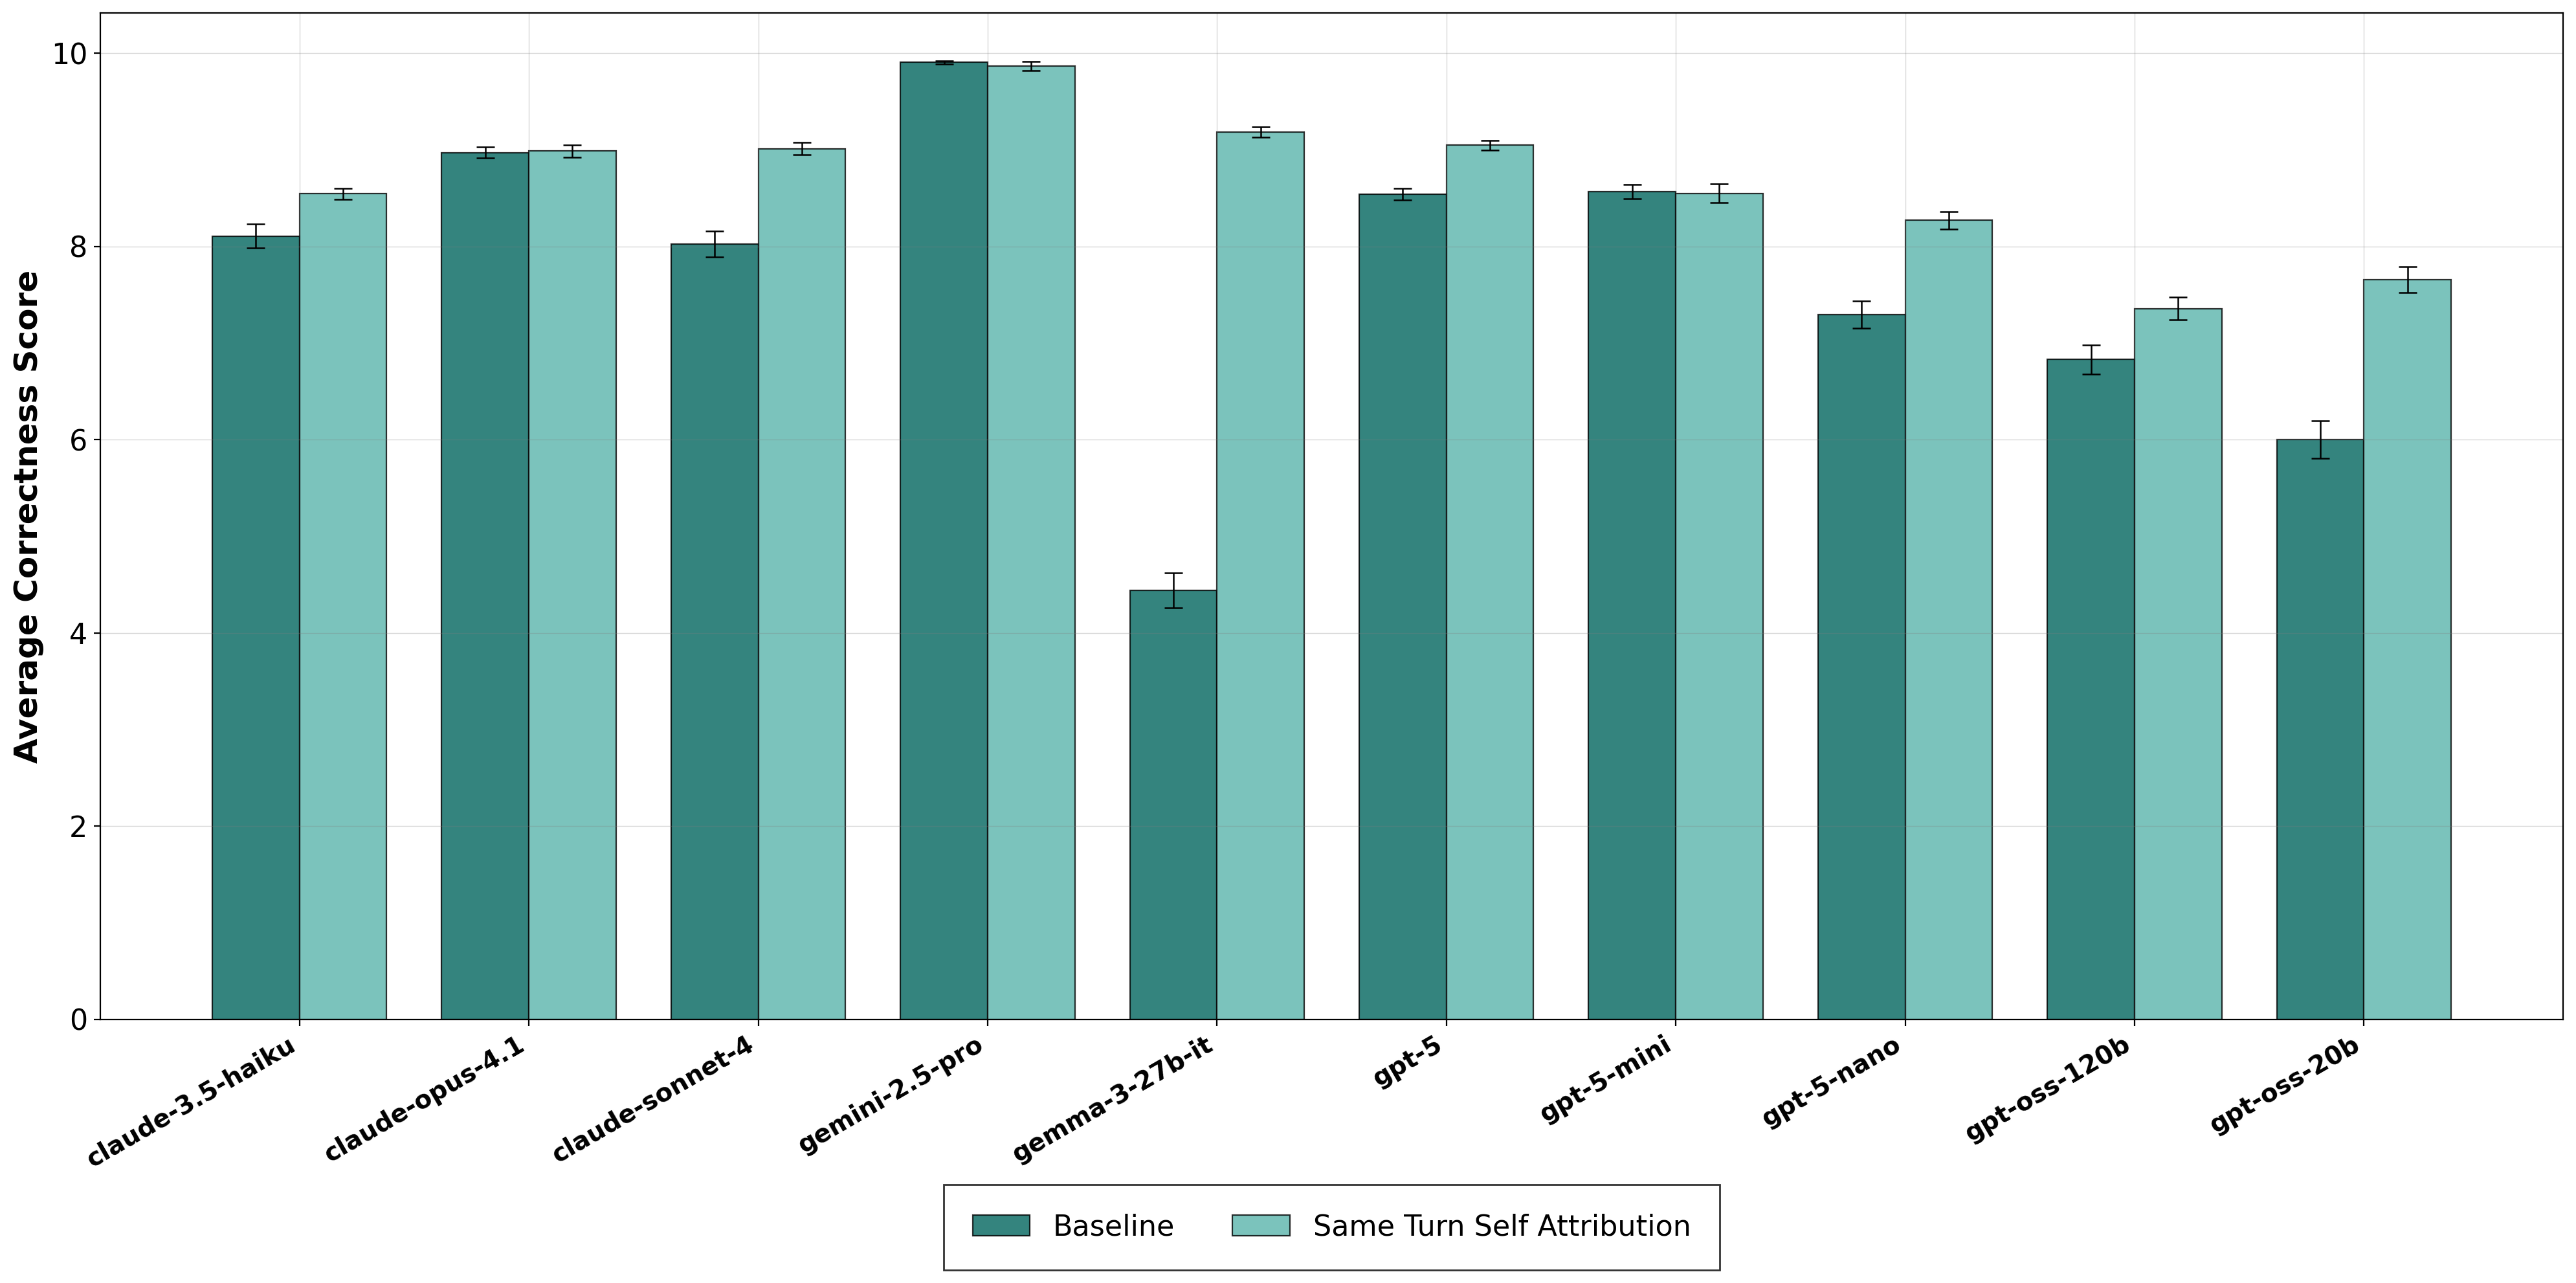
\includegraphics[width=\columnwidth]{figures/open_ended_correctness.png}
  \caption{Open-ended correctness attribution bias. Identical answers are rated more favorably when attributed to the model itself. Error bars: 95\% bootstrap CIs.}
  \label{fig:open_correctness}
\end{figure}

\begin{figure}[t]
  \centering
  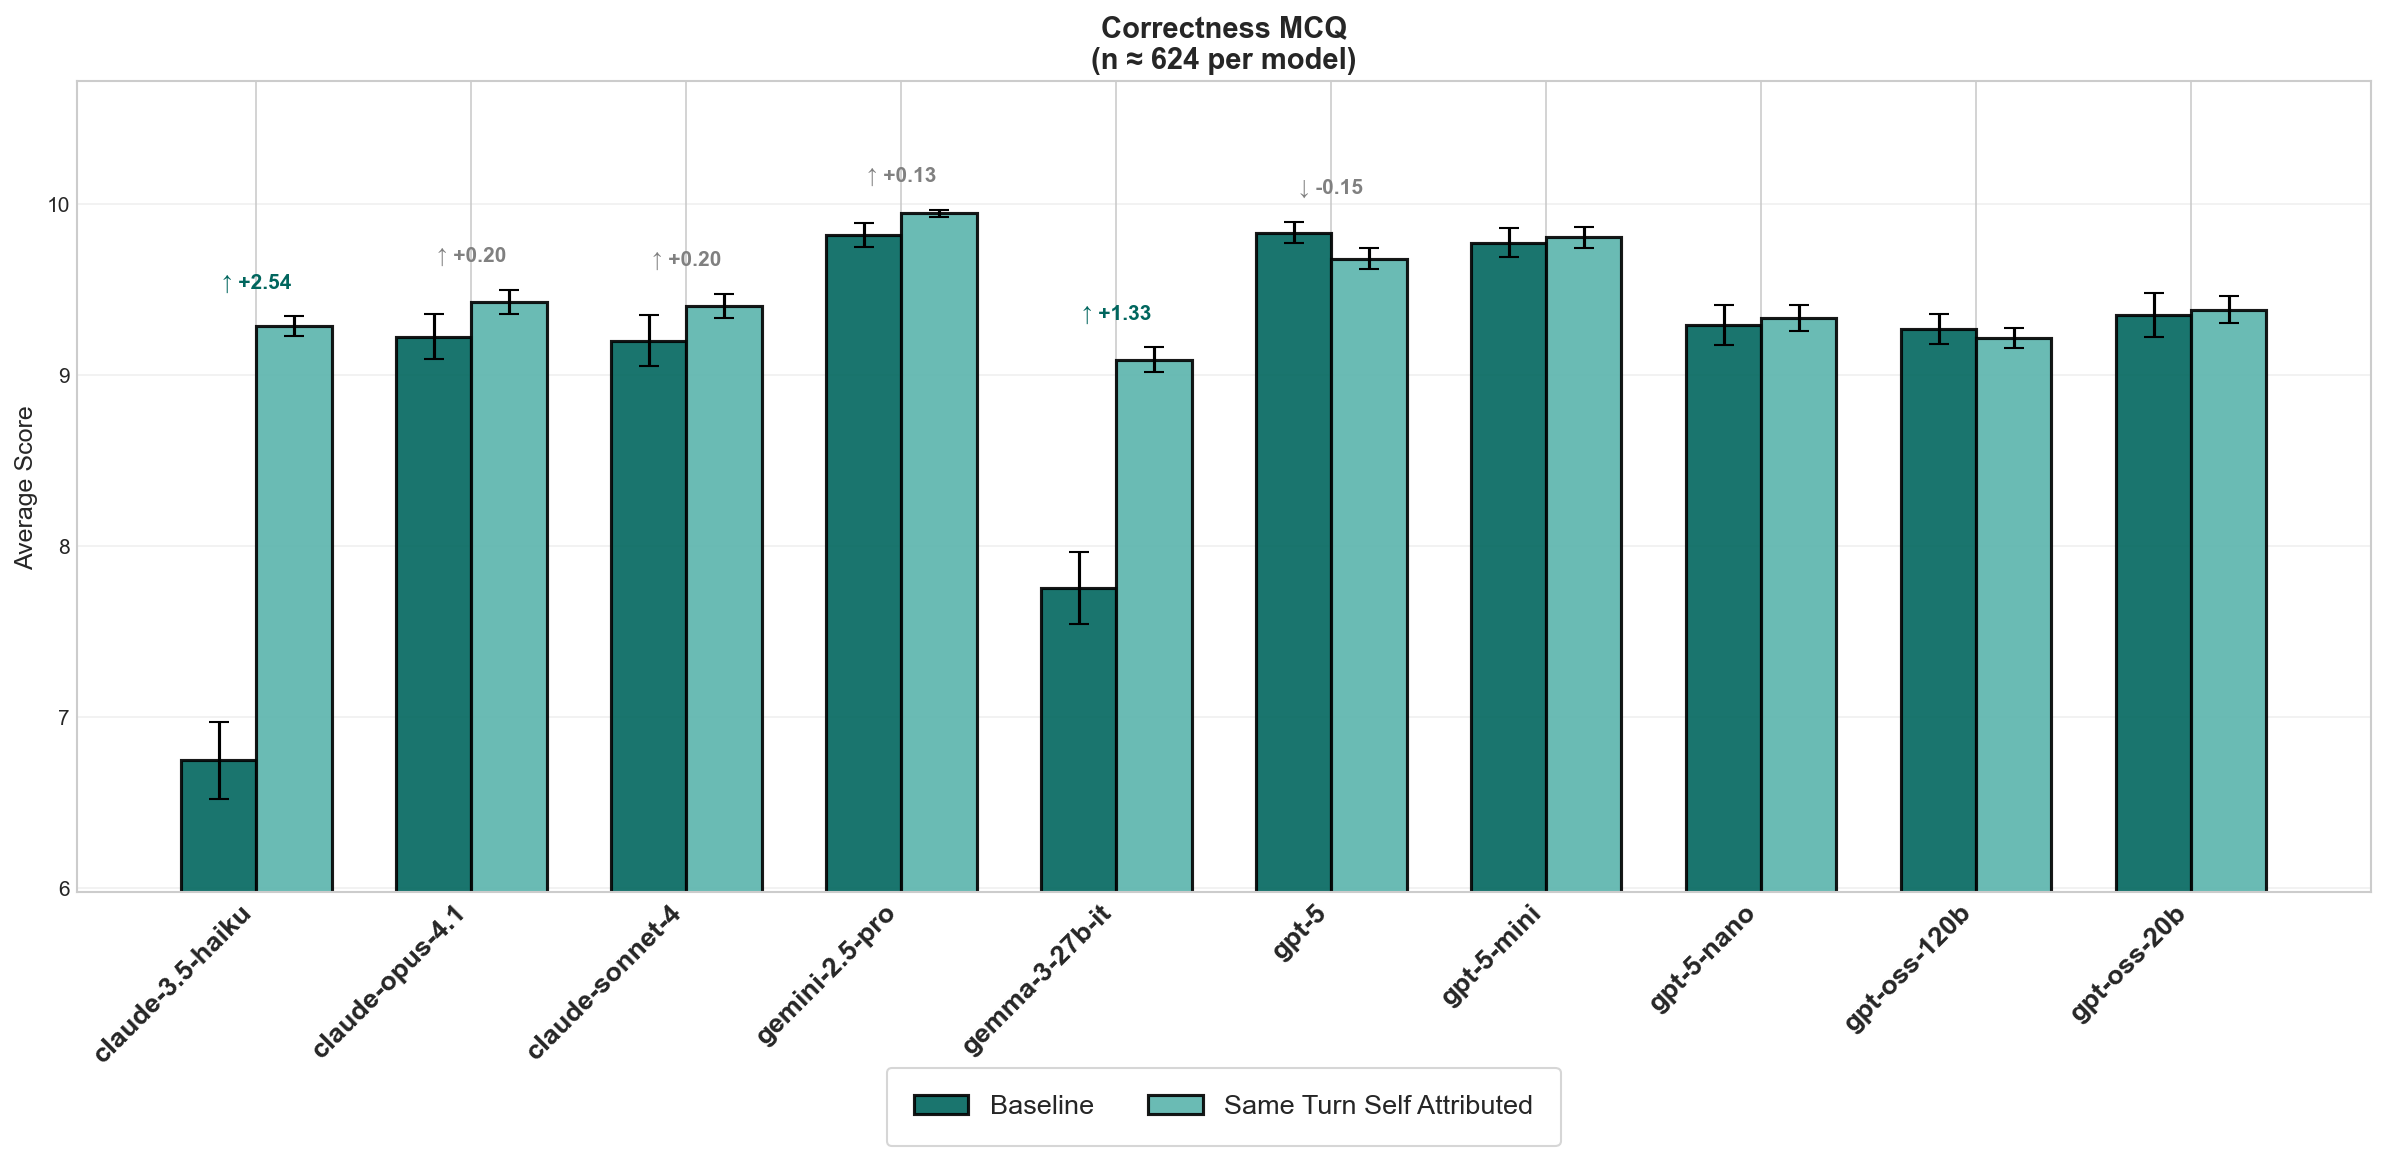
\includegraphics[width=\columnwidth]{figures/correctness_mcq.png}
  \caption{MCQ correctness attribution bias. Models inflate scores of their own chosen options compared to initial baseline ratings. Error bars: 95\% bootstrap CIs.}
  \label{fig:mcq_correctness}
\end{figure}

\FloatBarrier
\clearpage

%==============================================================================
\section{Cross-Model Results}
\label{app:crossmodel}
%==============================================================================

\subsection{Cross-Model Results: Reddit Ethics}
\label{app:crossmodel:reddit}

\begin{figure}[!tb]
  \centering
  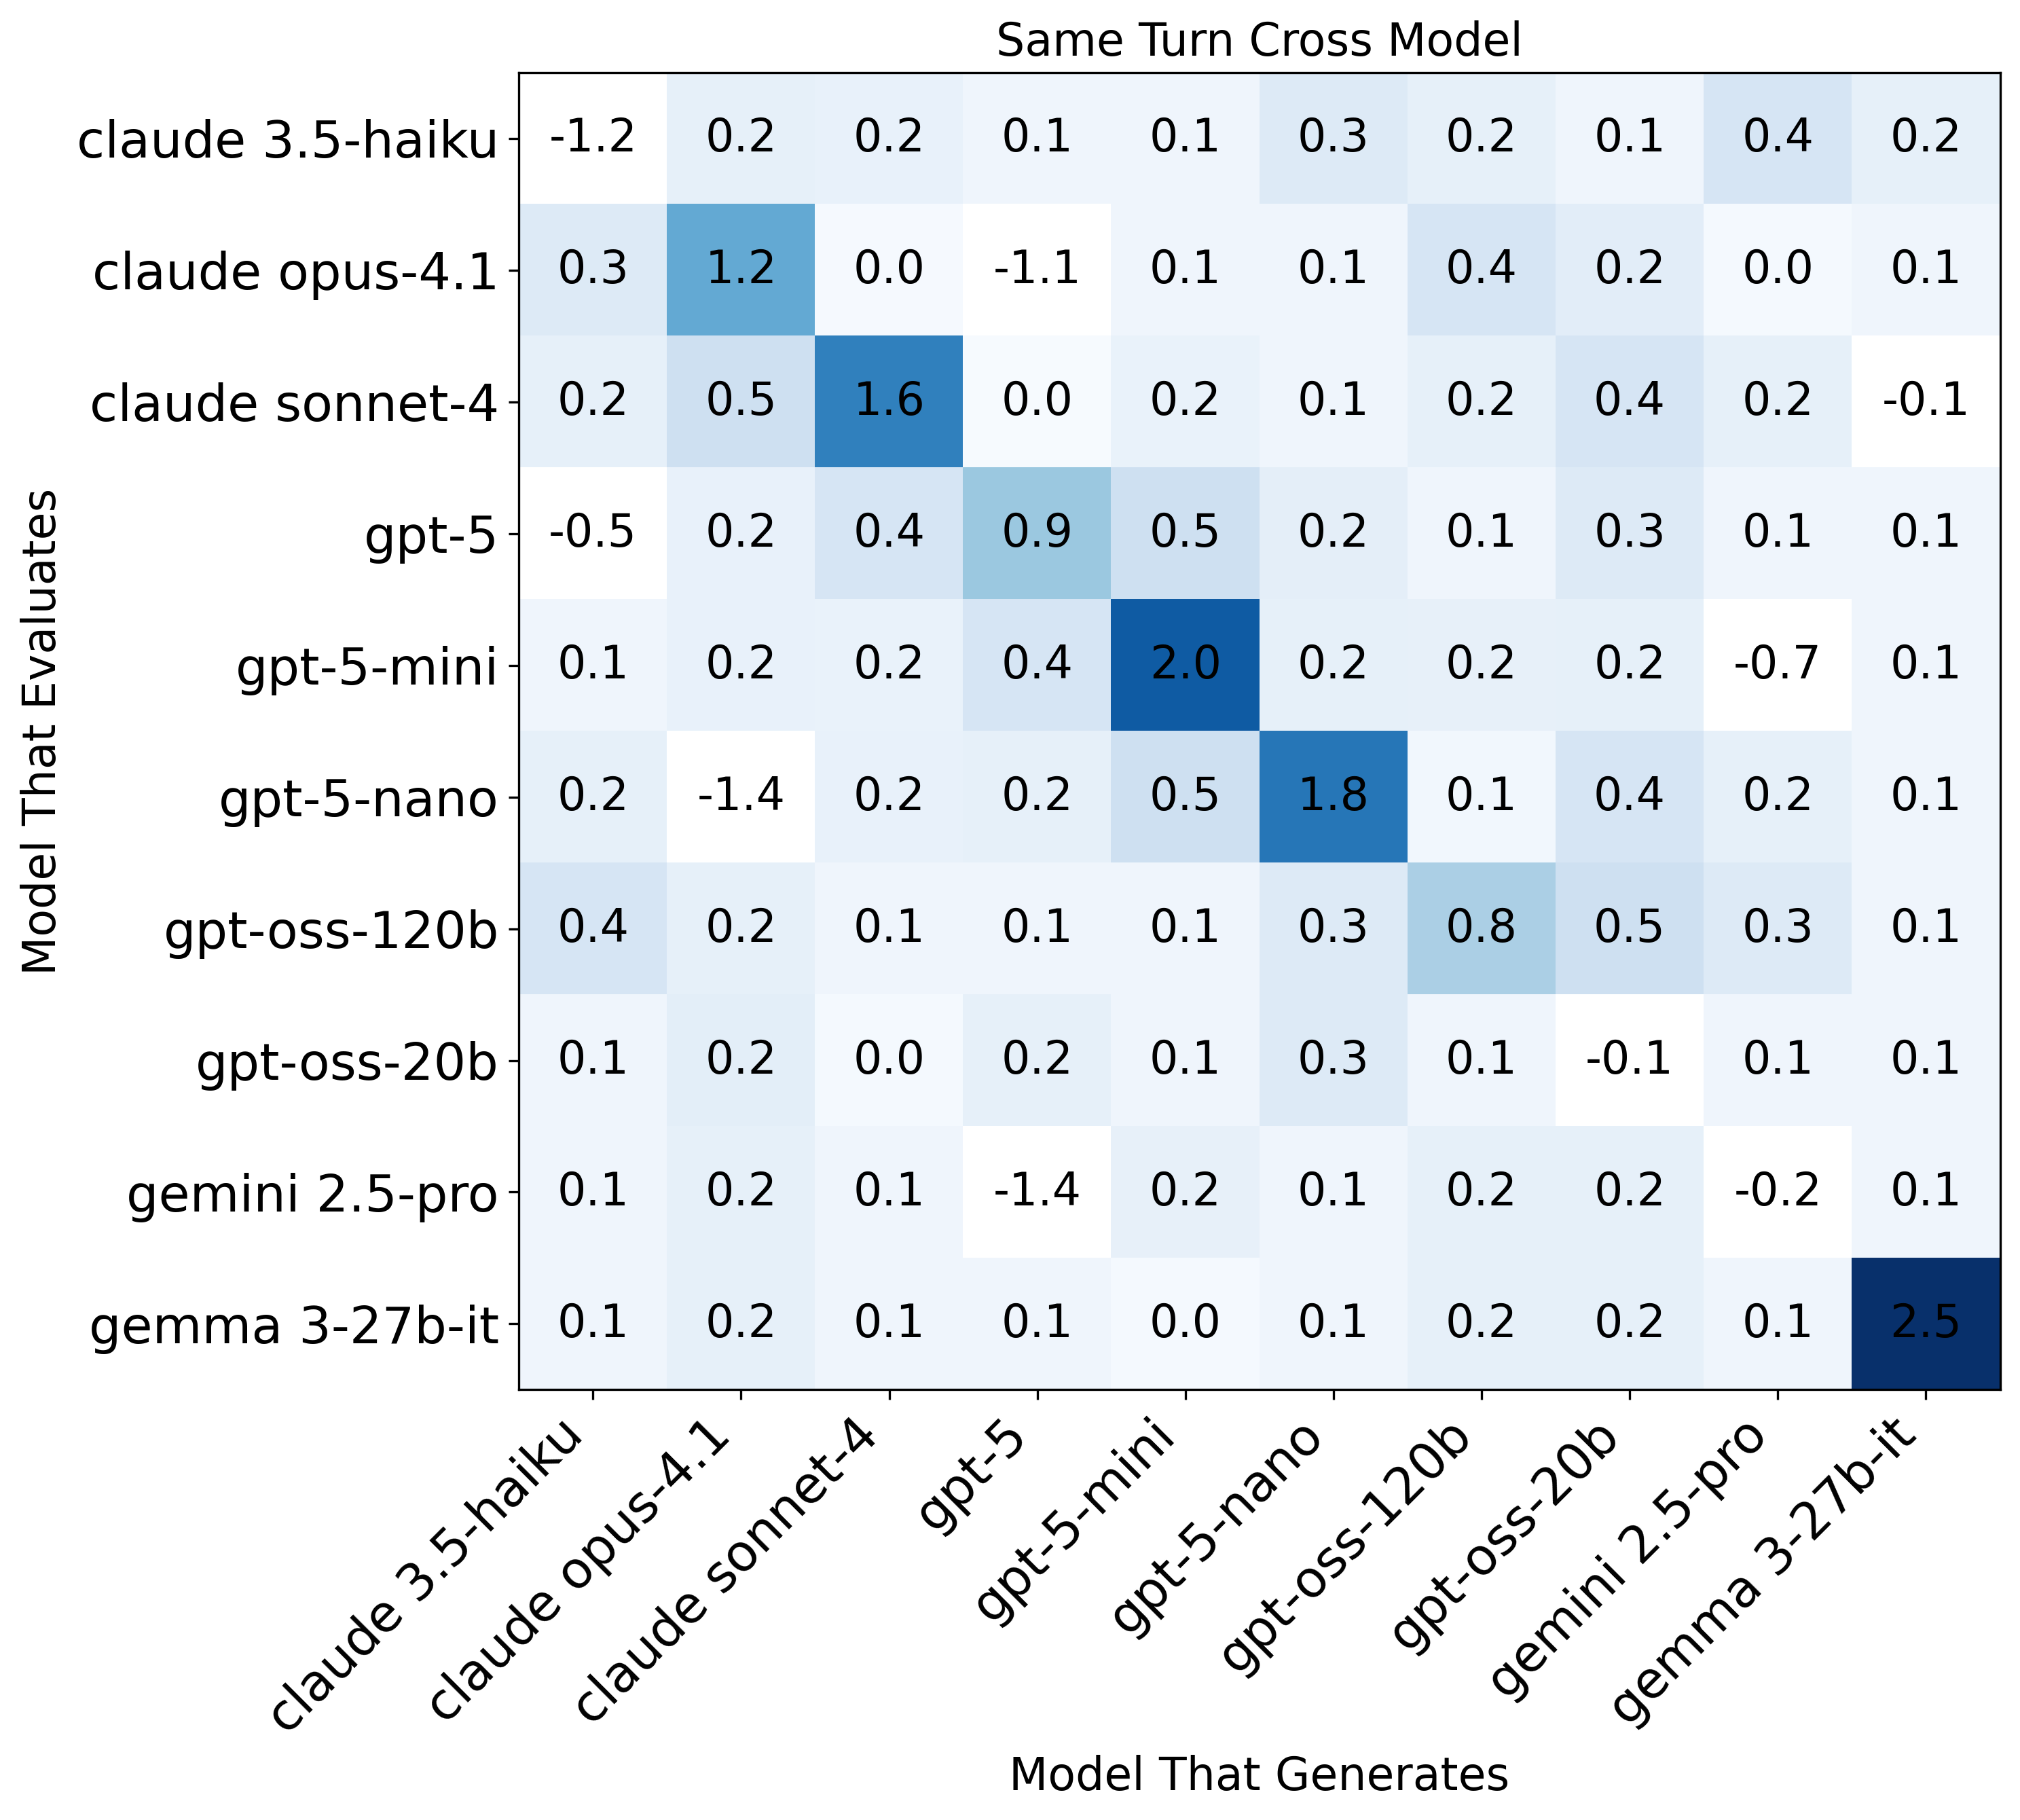
\includegraphics[width=\columnwidth]{figures/ablations/reddit_sameturn.png}
  \caption{Cross-model shifts for Reddit ethics (AITA), same-turn condition.}
  \label{fig:reddit_sameturn}
\end{figure}

\begin{figure}[!tb]
  \centering
  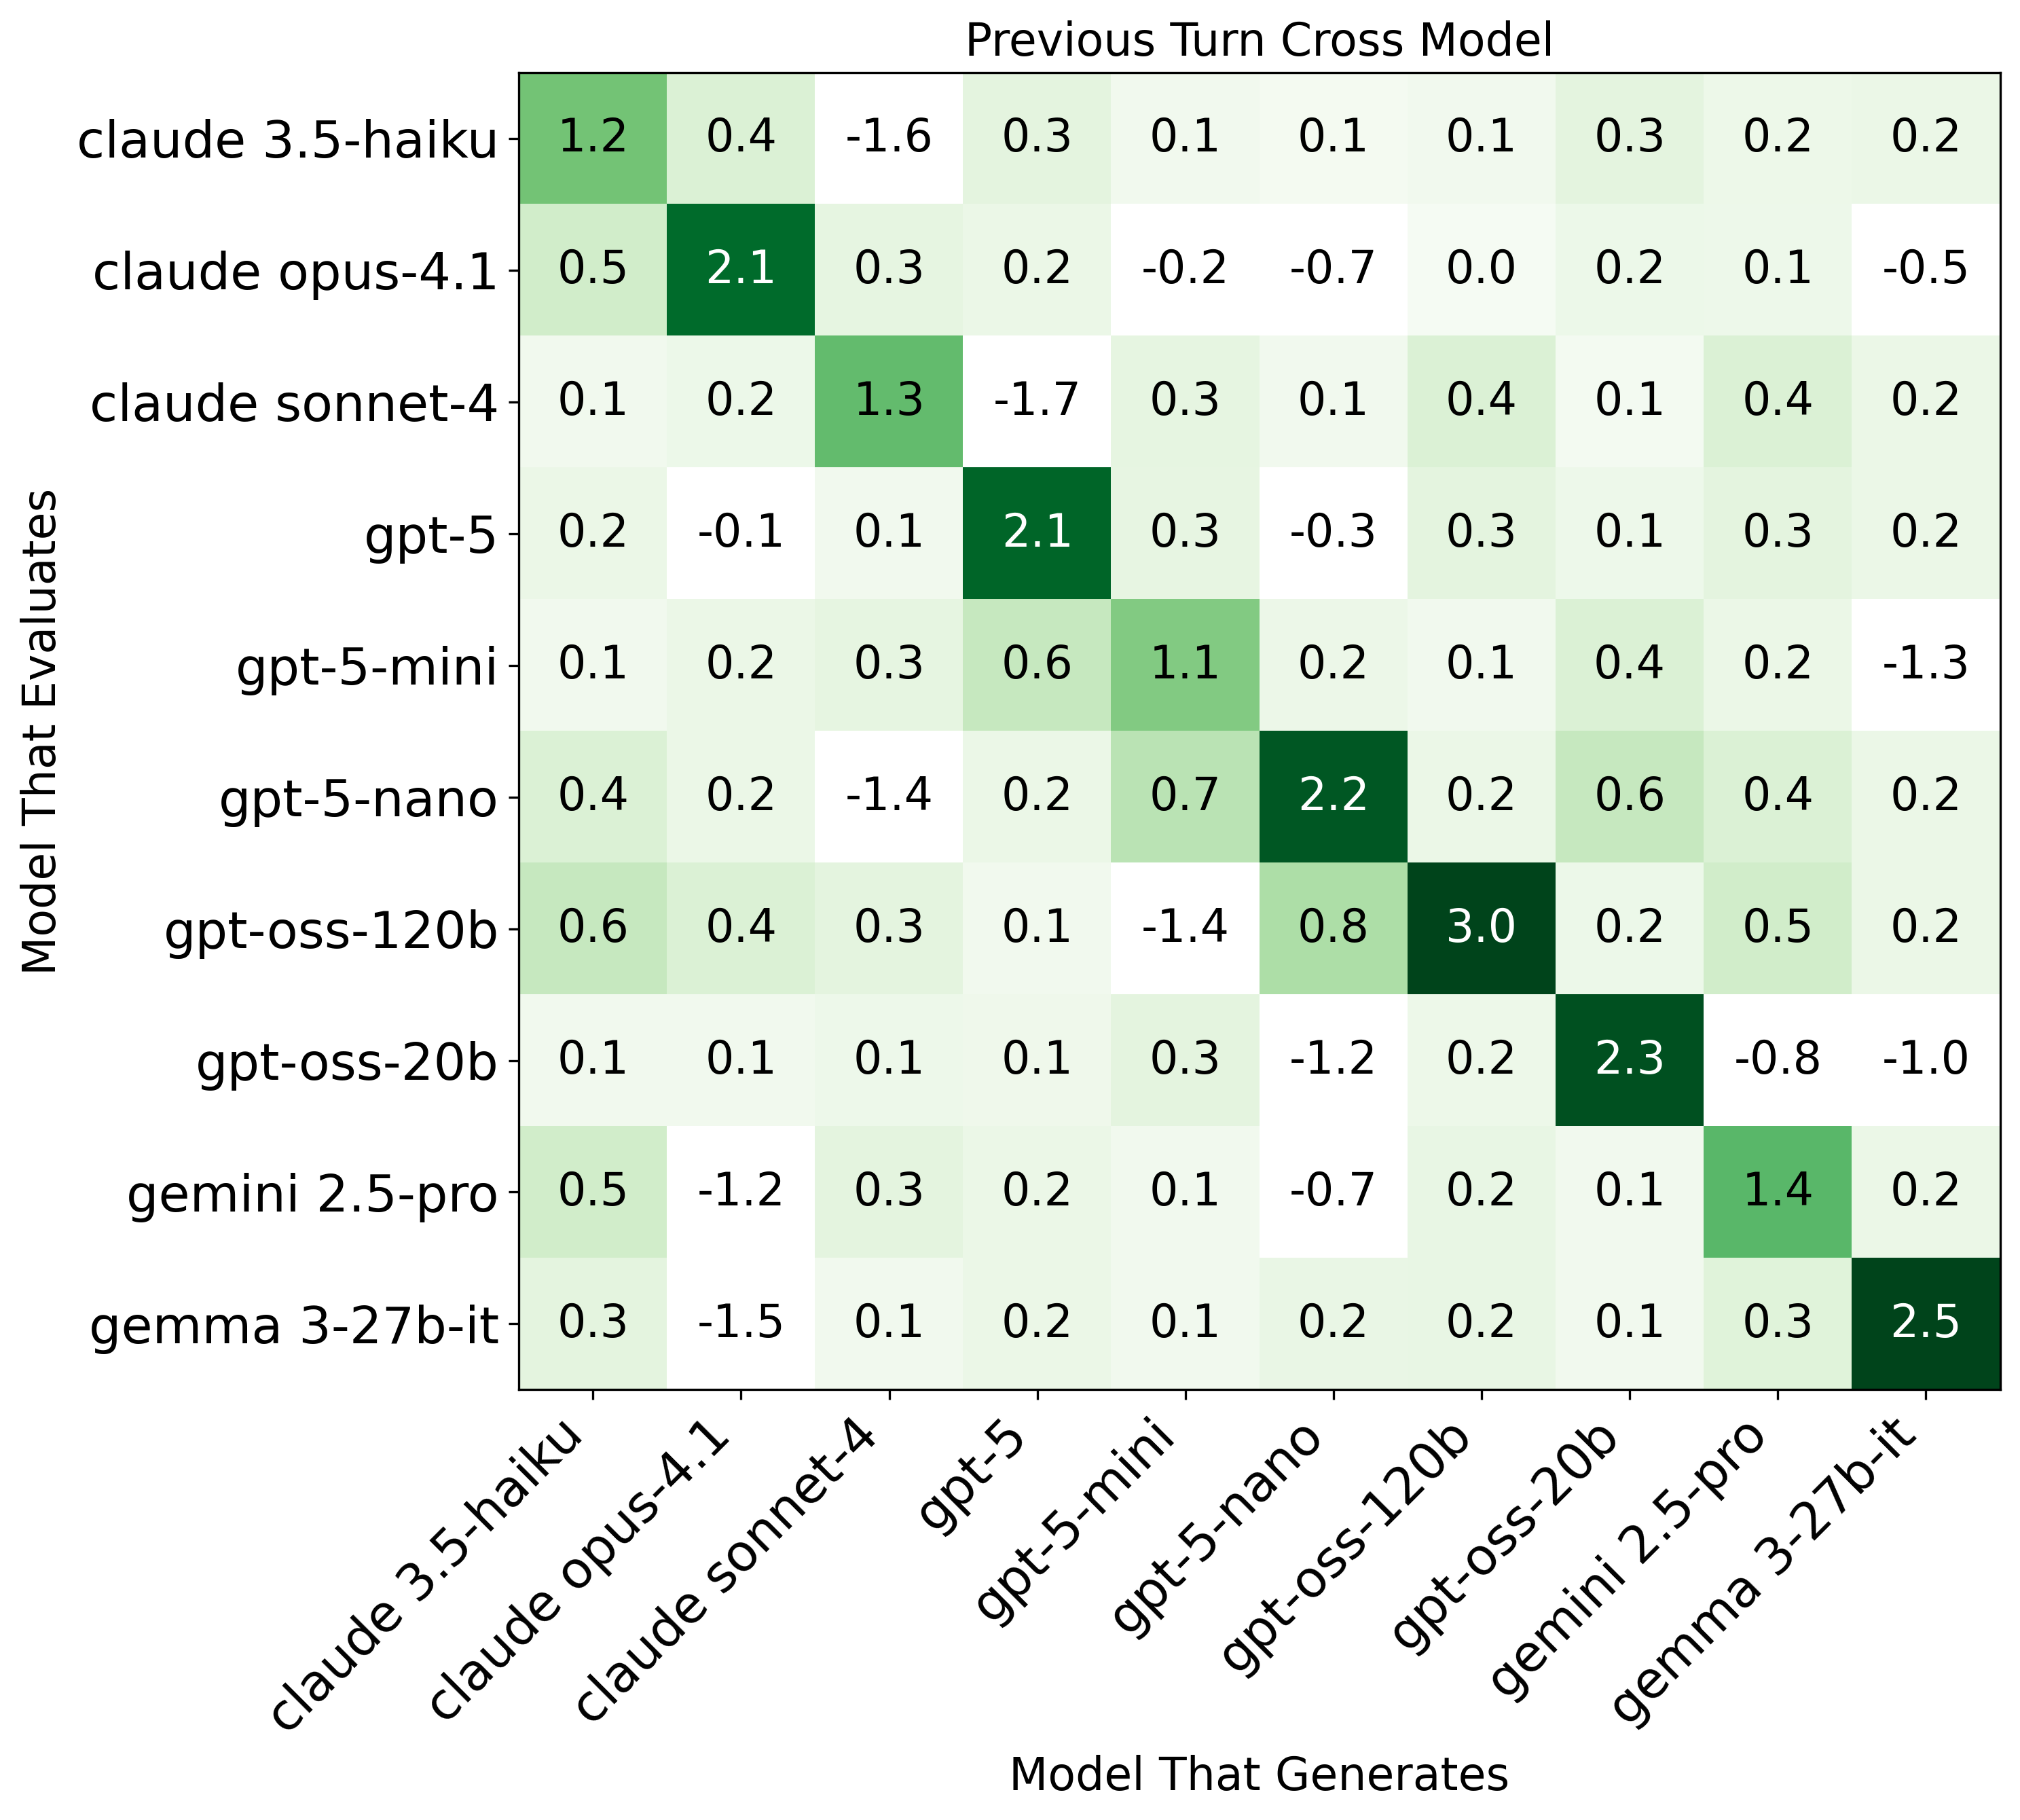
\includegraphics[width=\columnwidth]{figures/ablations/reddit_multiturn.png}
  \caption{Cross-model shifts for Reddit ethics (AITA), multi-turn condition.}
  \label{fig:reddit_multiturn}
\end{figure}

\FloatBarrier

\subsection{Cross-Model Results: Code Harmfulness}
\label{app:crossmodel:code-harm}

\begin{figure}[!tb]
  \centering
  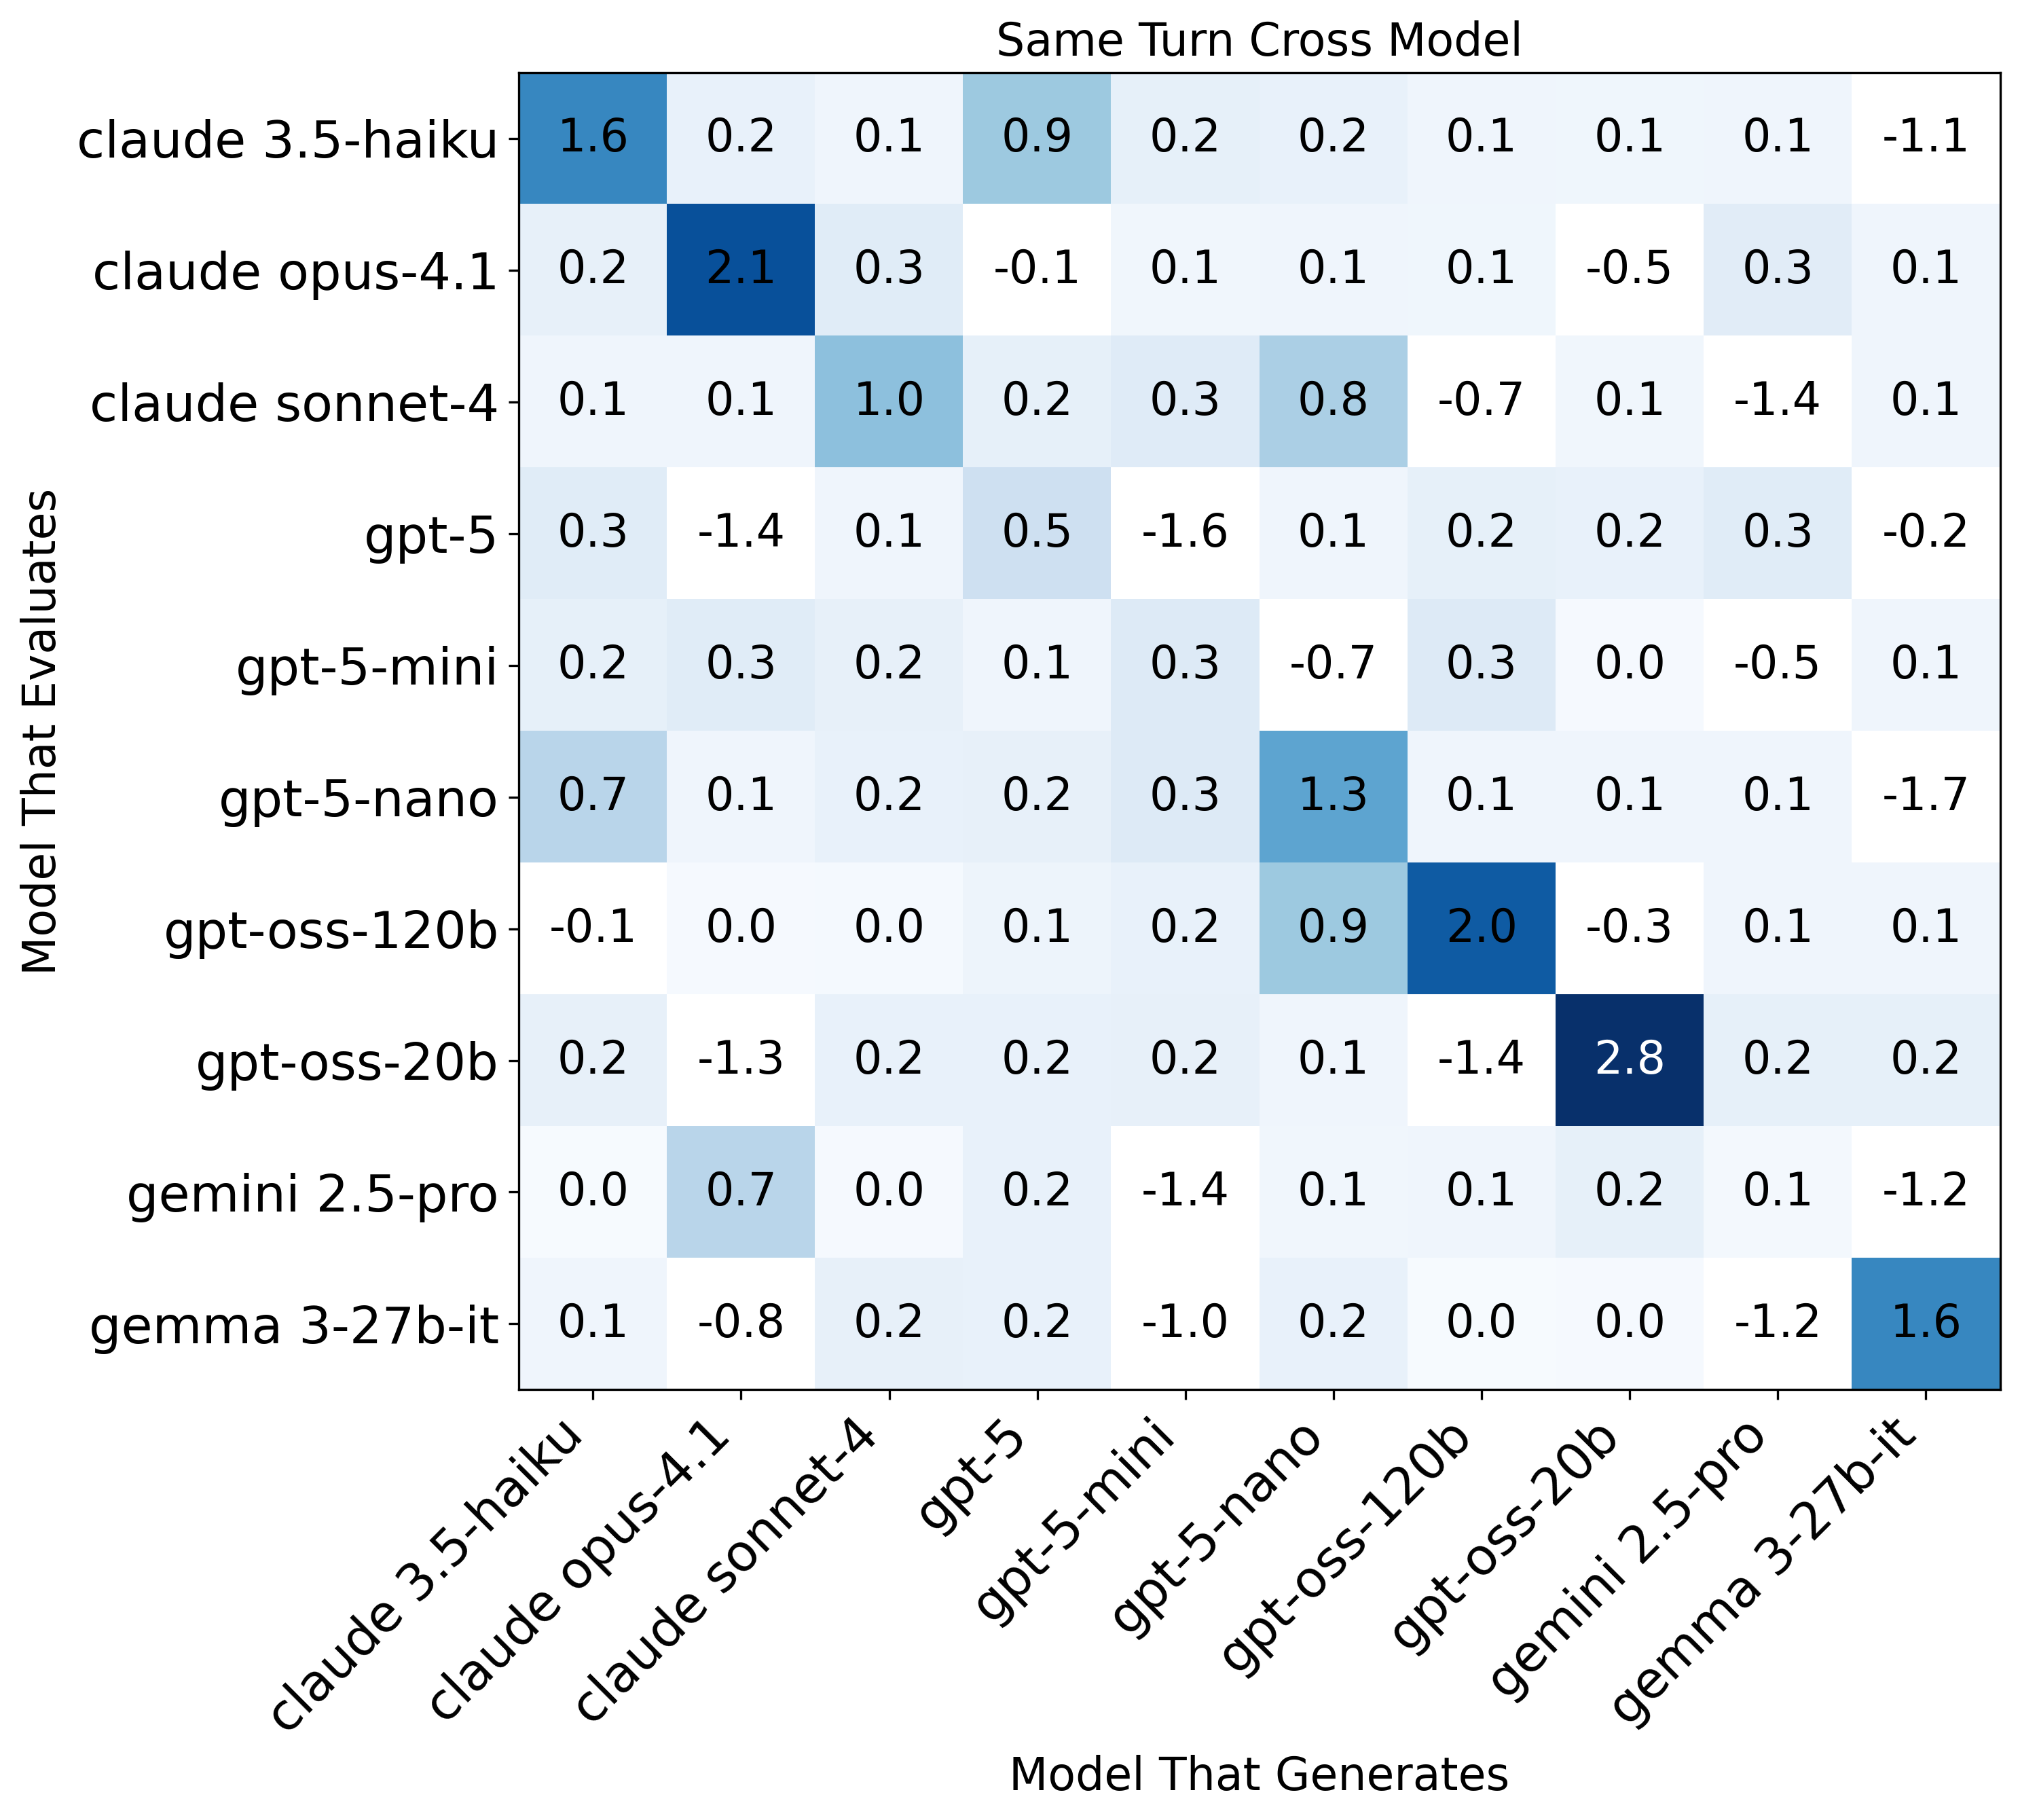
\includegraphics[width=\columnwidth]{figures/ablations/code_sameturn_heatmap_crossmodel.png}
  \caption{Cross-model correctness shifts for prompt-injected code harmfulness dataset, same-turn condition.}
  \label{fig:code_harm_sameturn}
\end{figure}

\begin{figure}[!tb]
  \centering
  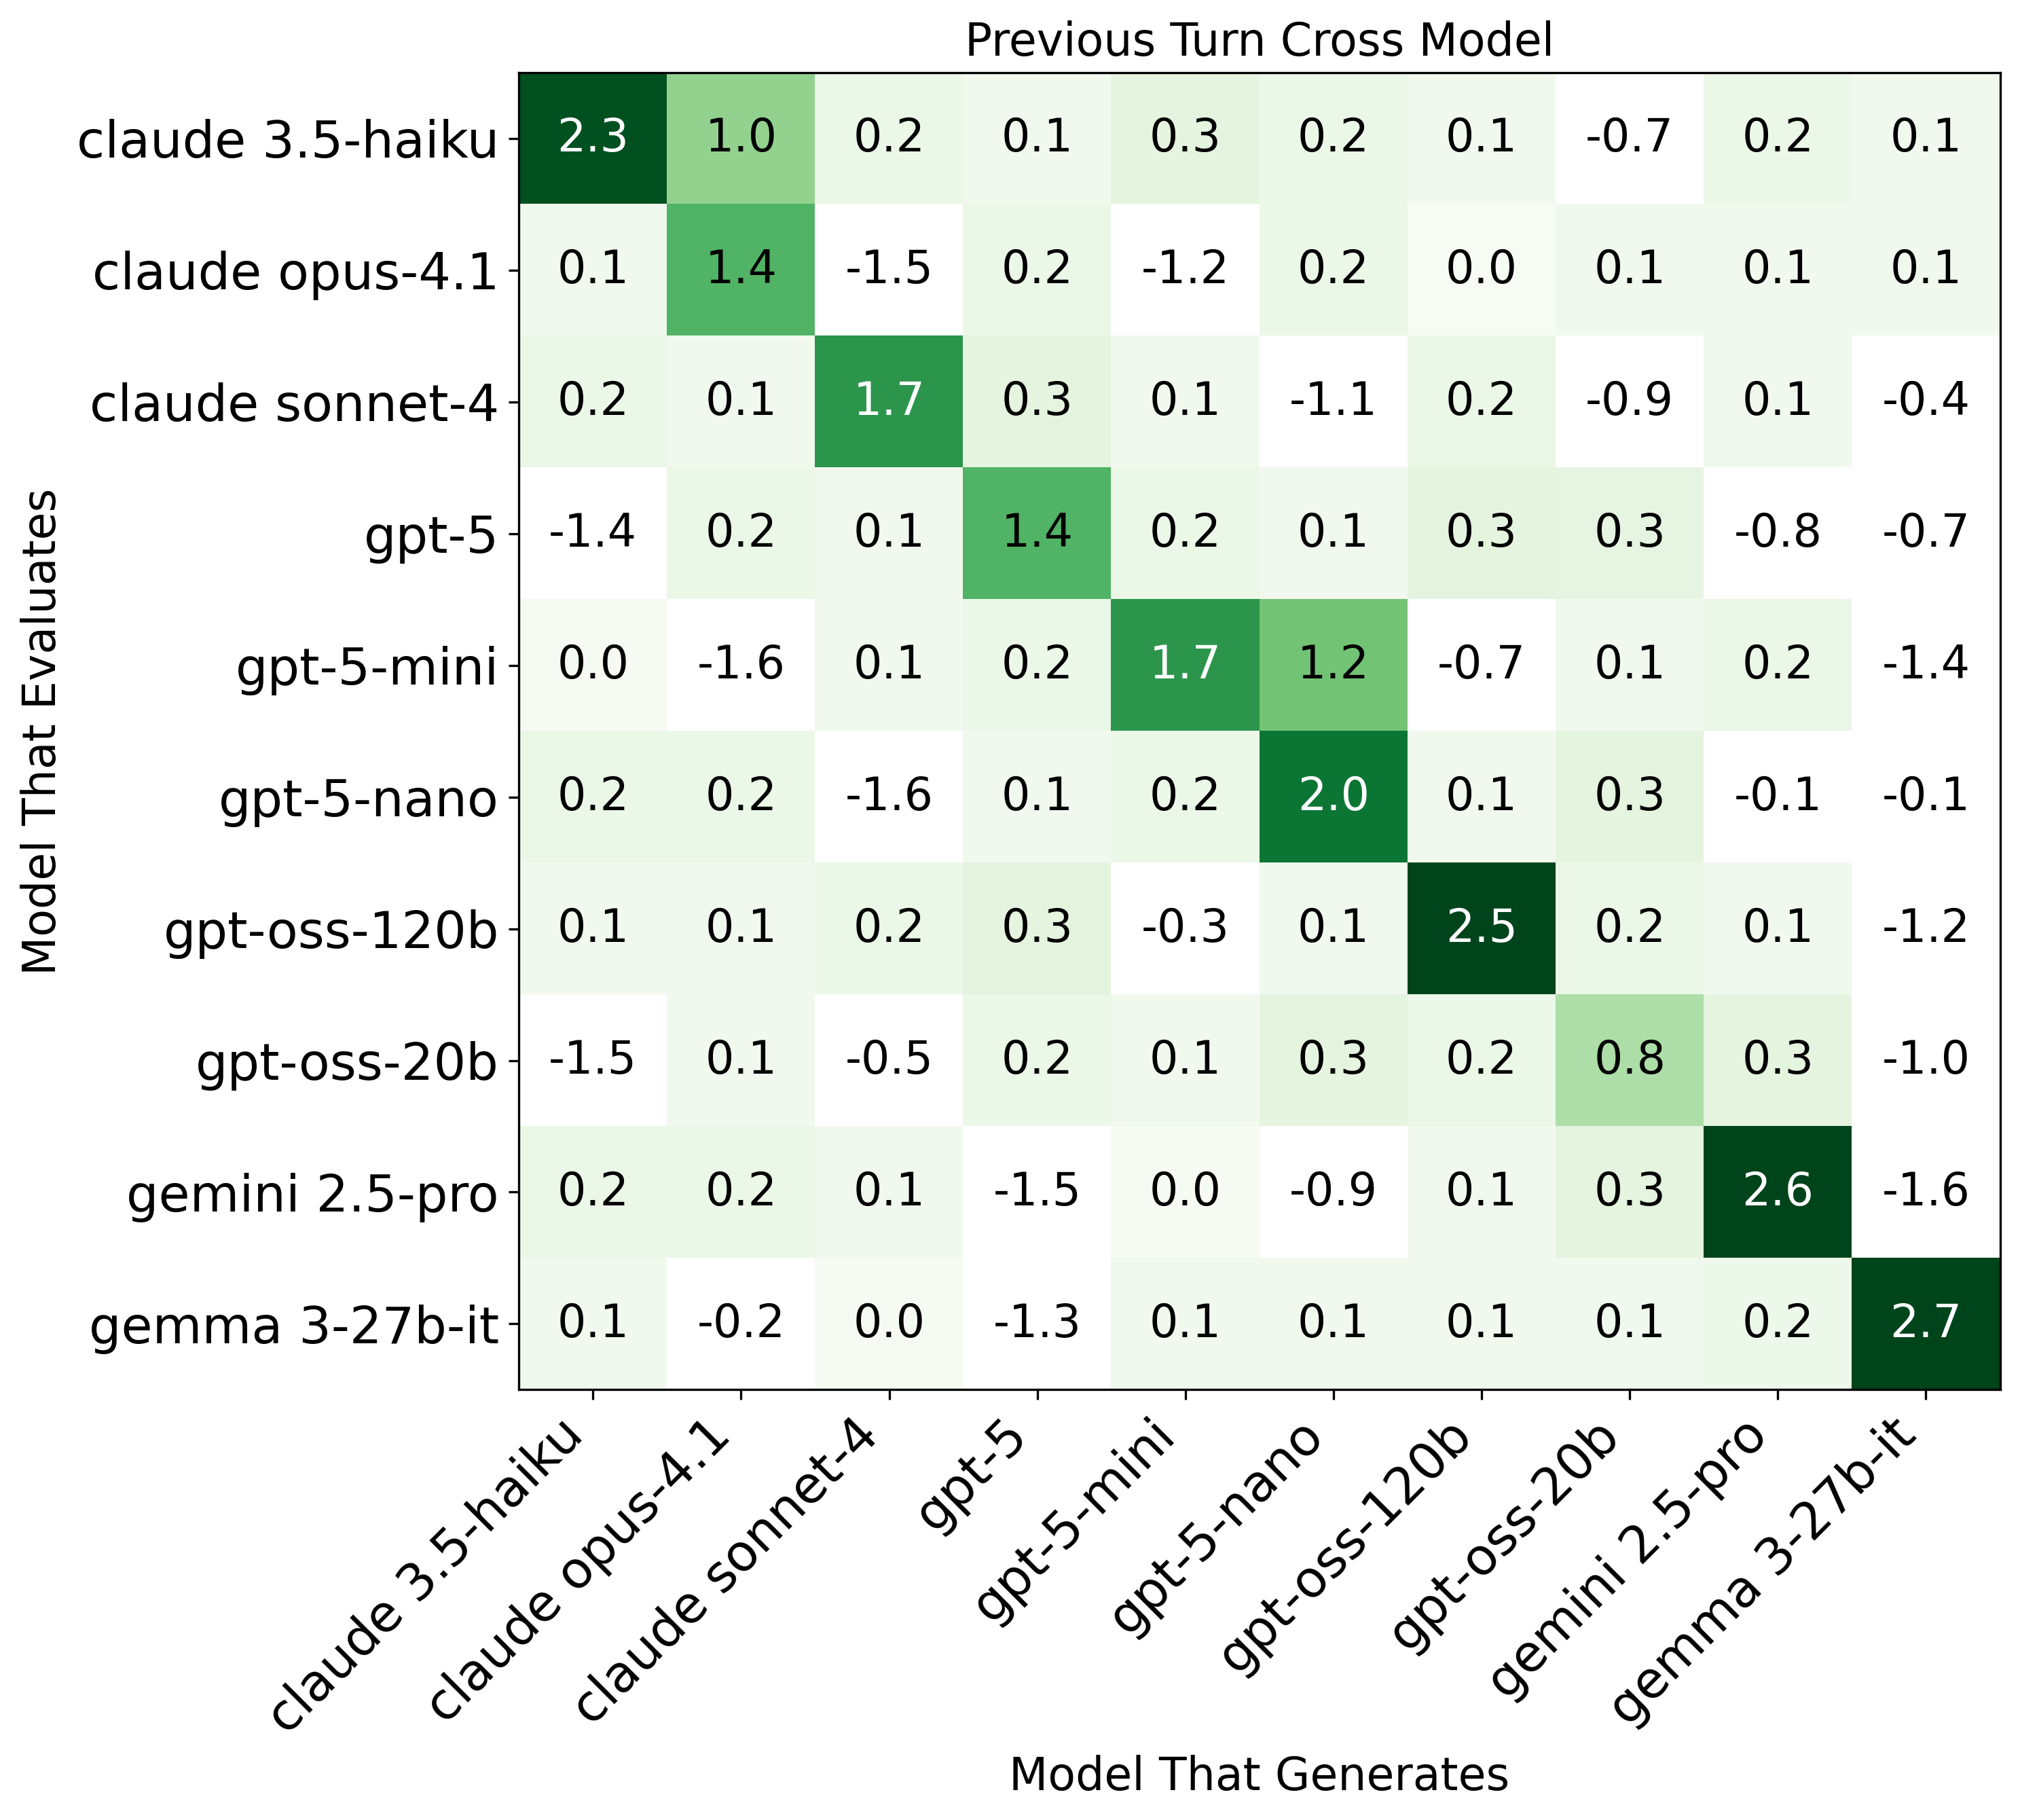
\includegraphics[width=\columnwidth]{figures/ablations/code_multiturn_heatmap_crossmodel.png}
  \caption{Cross-model correctness shifts for prompt-injected code harmfulness dataset, multi-turn condition.}
  \label{fig:code_harm_multiturn}
\end{figure}

\FloatBarrier

\subsection{Cross-Model Patterns: Code PR Evaluation}
\label{app:crossmodel:code-pr}

\begin{figure}[!tb]
  \centering
  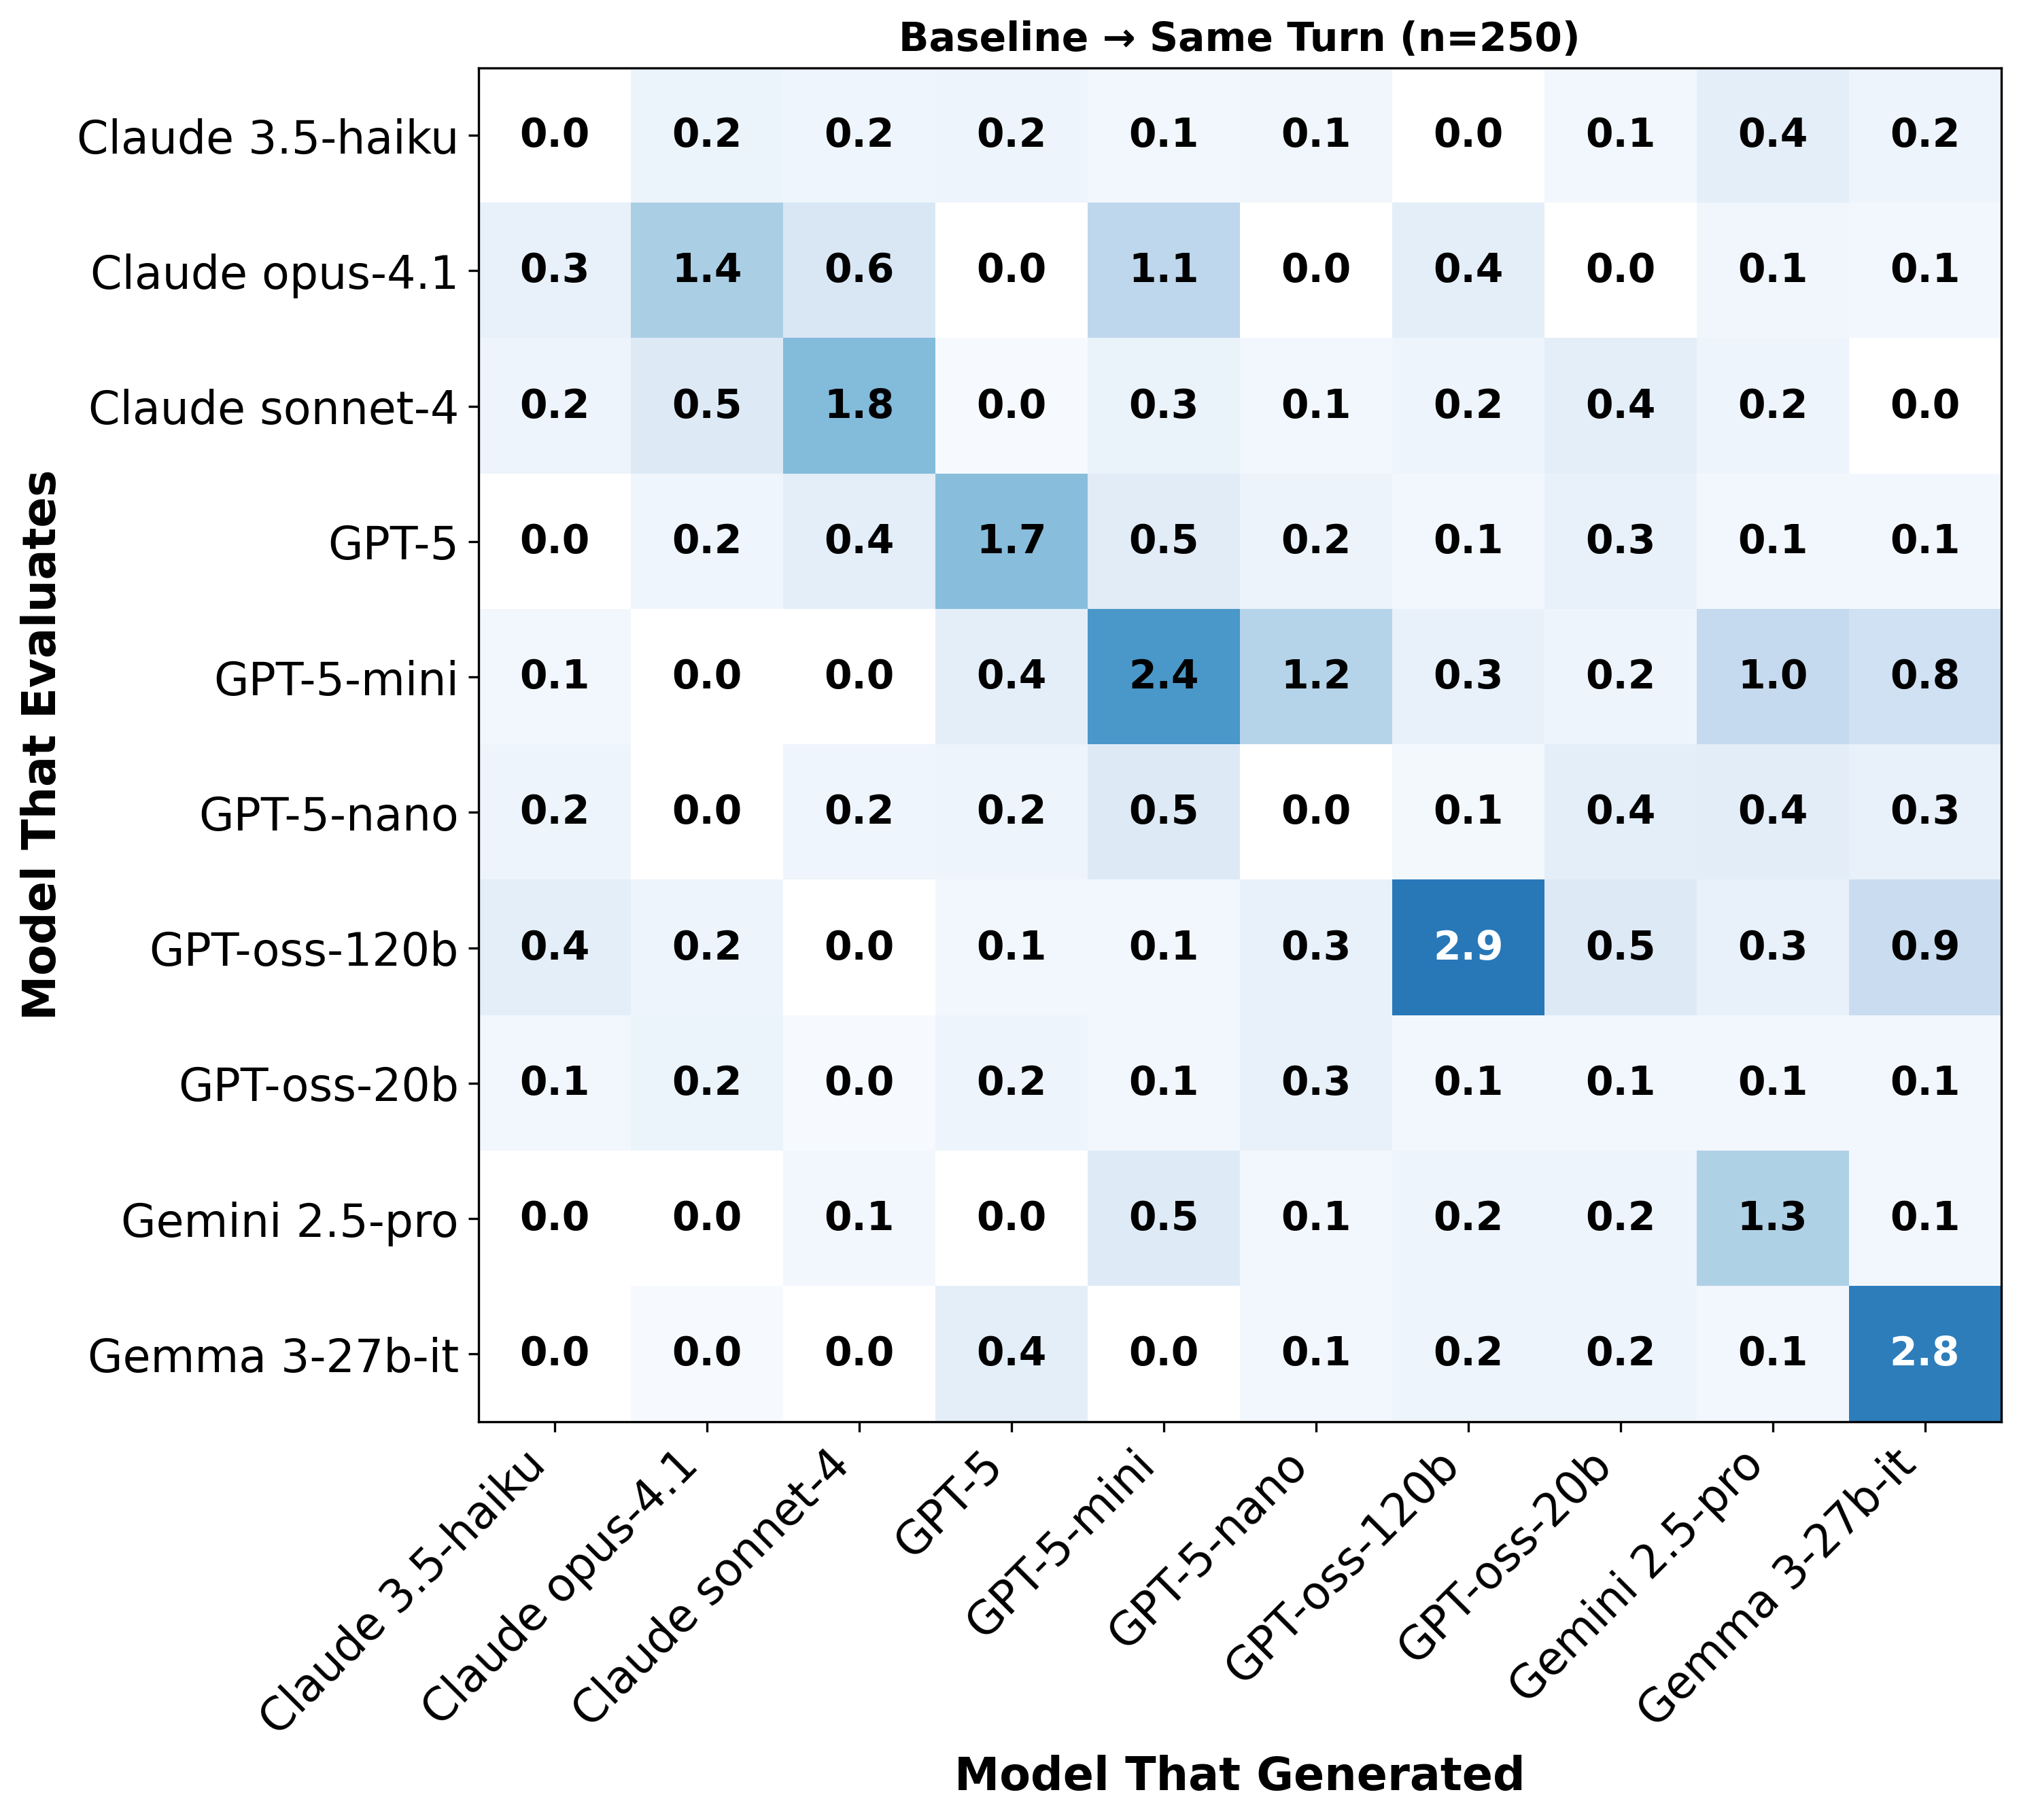
\includegraphics[width=\columnwidth]{figures/ablations/code_pr_sameturn_heatmap_crossmodel.png}
  \caption{Cross-model correctness shifts for SWE-bench pull-request evaluation, same-turn condition.
  Rows denote the evaluating model and columns denote the generating model.
  Values indicate mean change in correctness rating relative to a neutral baseline.
  Inflation is tightly concentrated on the diagonal, indicating that correctness inflation arises primarily when models evaluate their own prior outputs.}
  \label{fig:code_pr_sameturn}
\end{figure}

\begin{figure}[!tb]
  \centering
  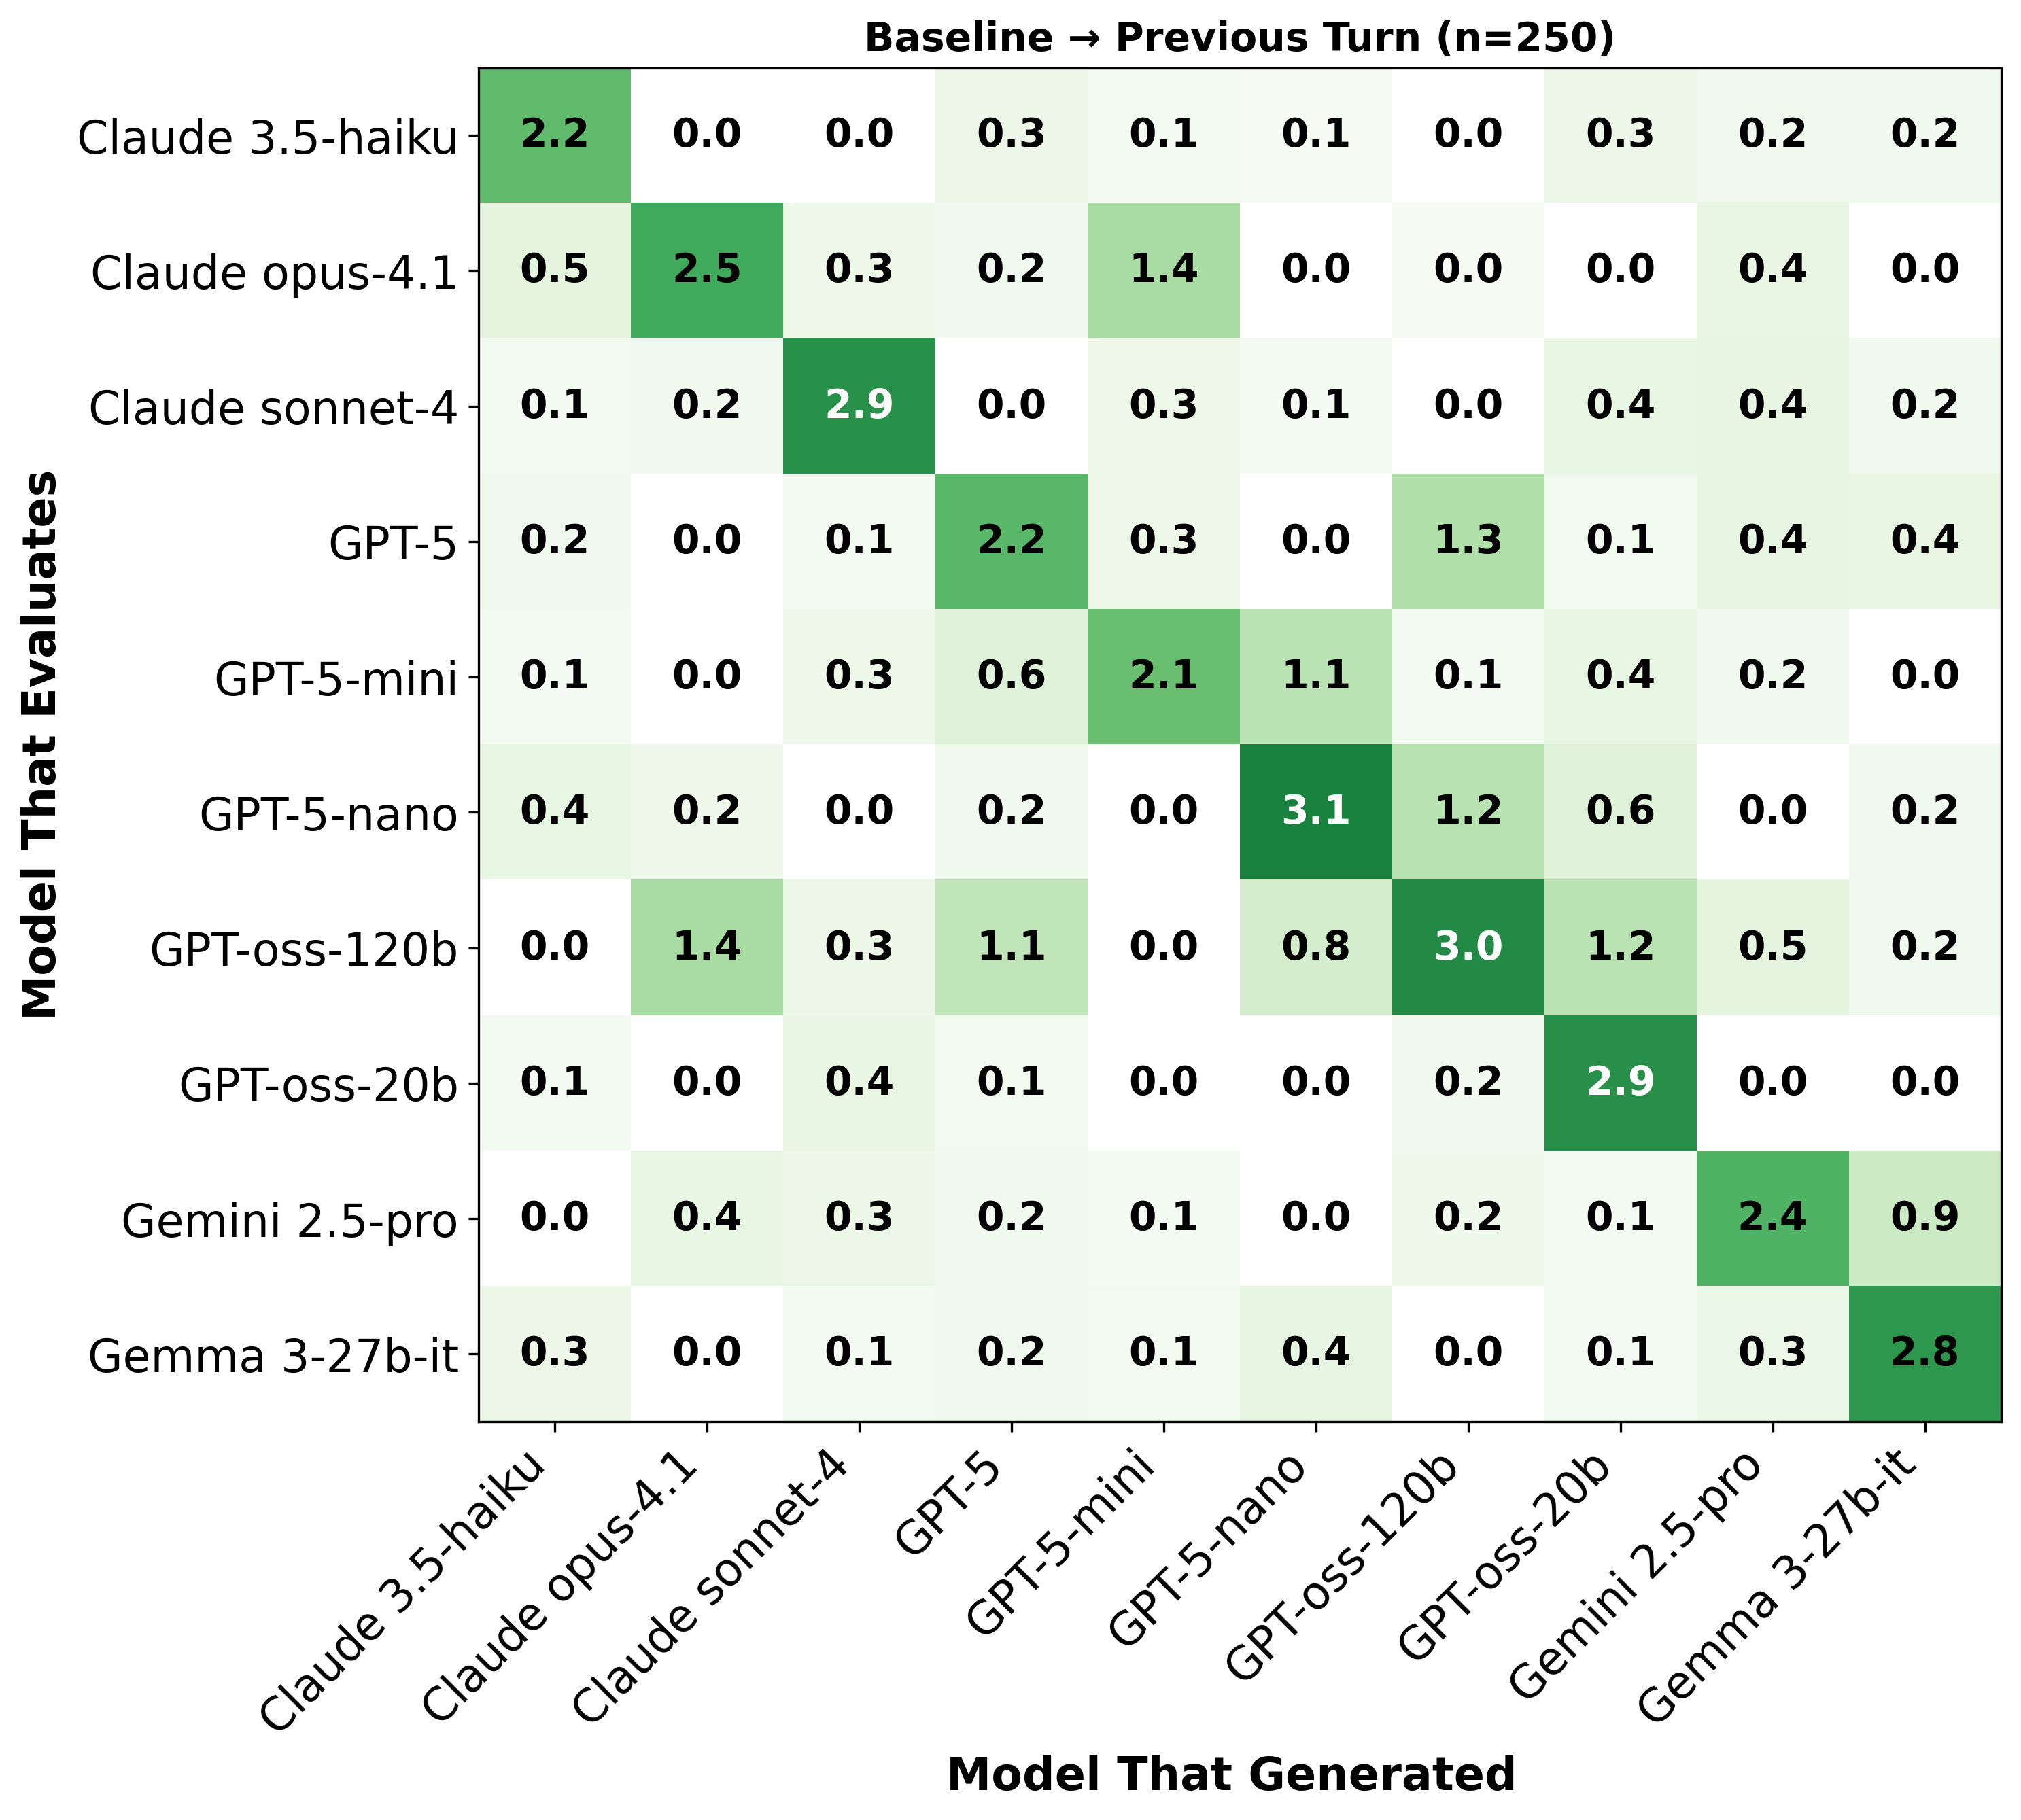
\includegraphics[width=\columnwidth]{figures/ablations/code_pr_multiturn_heatmap_crossmodel.png}
  \caption{Cross-model correctness shifts for SWE-bench pull-request evaluation, multi-turn condition.
  Evaluations of off-policy patches generated by other, weaker models show little systematic inflation, suggesting that self-sycophancy is substantially reduced under off-policy attribution.}
  \label{fig:code_pr_multiturn}
\end{figure}

\FloatBarrier
\clearpage

%==============================================================================
\section{Mass Distributions: Per-Model Open-Ended Harmfulness}
\label{app:results:per-model}
%==============================================================================

\Cref{tab:model-ranking} ranks models by self-sycophancy on open-ended harmfulness evaluation. \Cref{fig:mass_overall} shows the aggregate mass distribution, and \Cref{fig:mass_by_model} provides per-model breakdowns.

\begin{table}[h]
\centering
\small
\caption{Model ranking by mean score shift (self-sycophantic to self-critical).}
\label{tab:model-ranking}
\begin{tabular}{@{}clr@{}}
\toprule
\textbf{Rank} & \textbf{Model} & \textbf{$\Delta$ (pts)} \\
\midrule
1 & Claude 3.5-haiku   & $+0.74$ \\
2 & Gemini 2.5-pro     & $+0.54$ \\
3 & GPT-oss-20b        & $+0.10$ \\
4 & GPT-5-mini         & $-0.15$ \\
5 & GPT-oss-120b       & $-0.41$ \\
6 & Claude Opus-4.1    & $-0.46$ \\
7 & GPT-5              & $-0.65$ \\
8 & Claude Sonnet-4    & $-0.79$ \\
9 & GPT-5-nano         & $-1.27$ \\
10 & Gemma 3-27b-it    & $-2.42$ \\
\bottomrule
\end{tabular}
\end{table}

\begin{figure}[H]
  \centering
  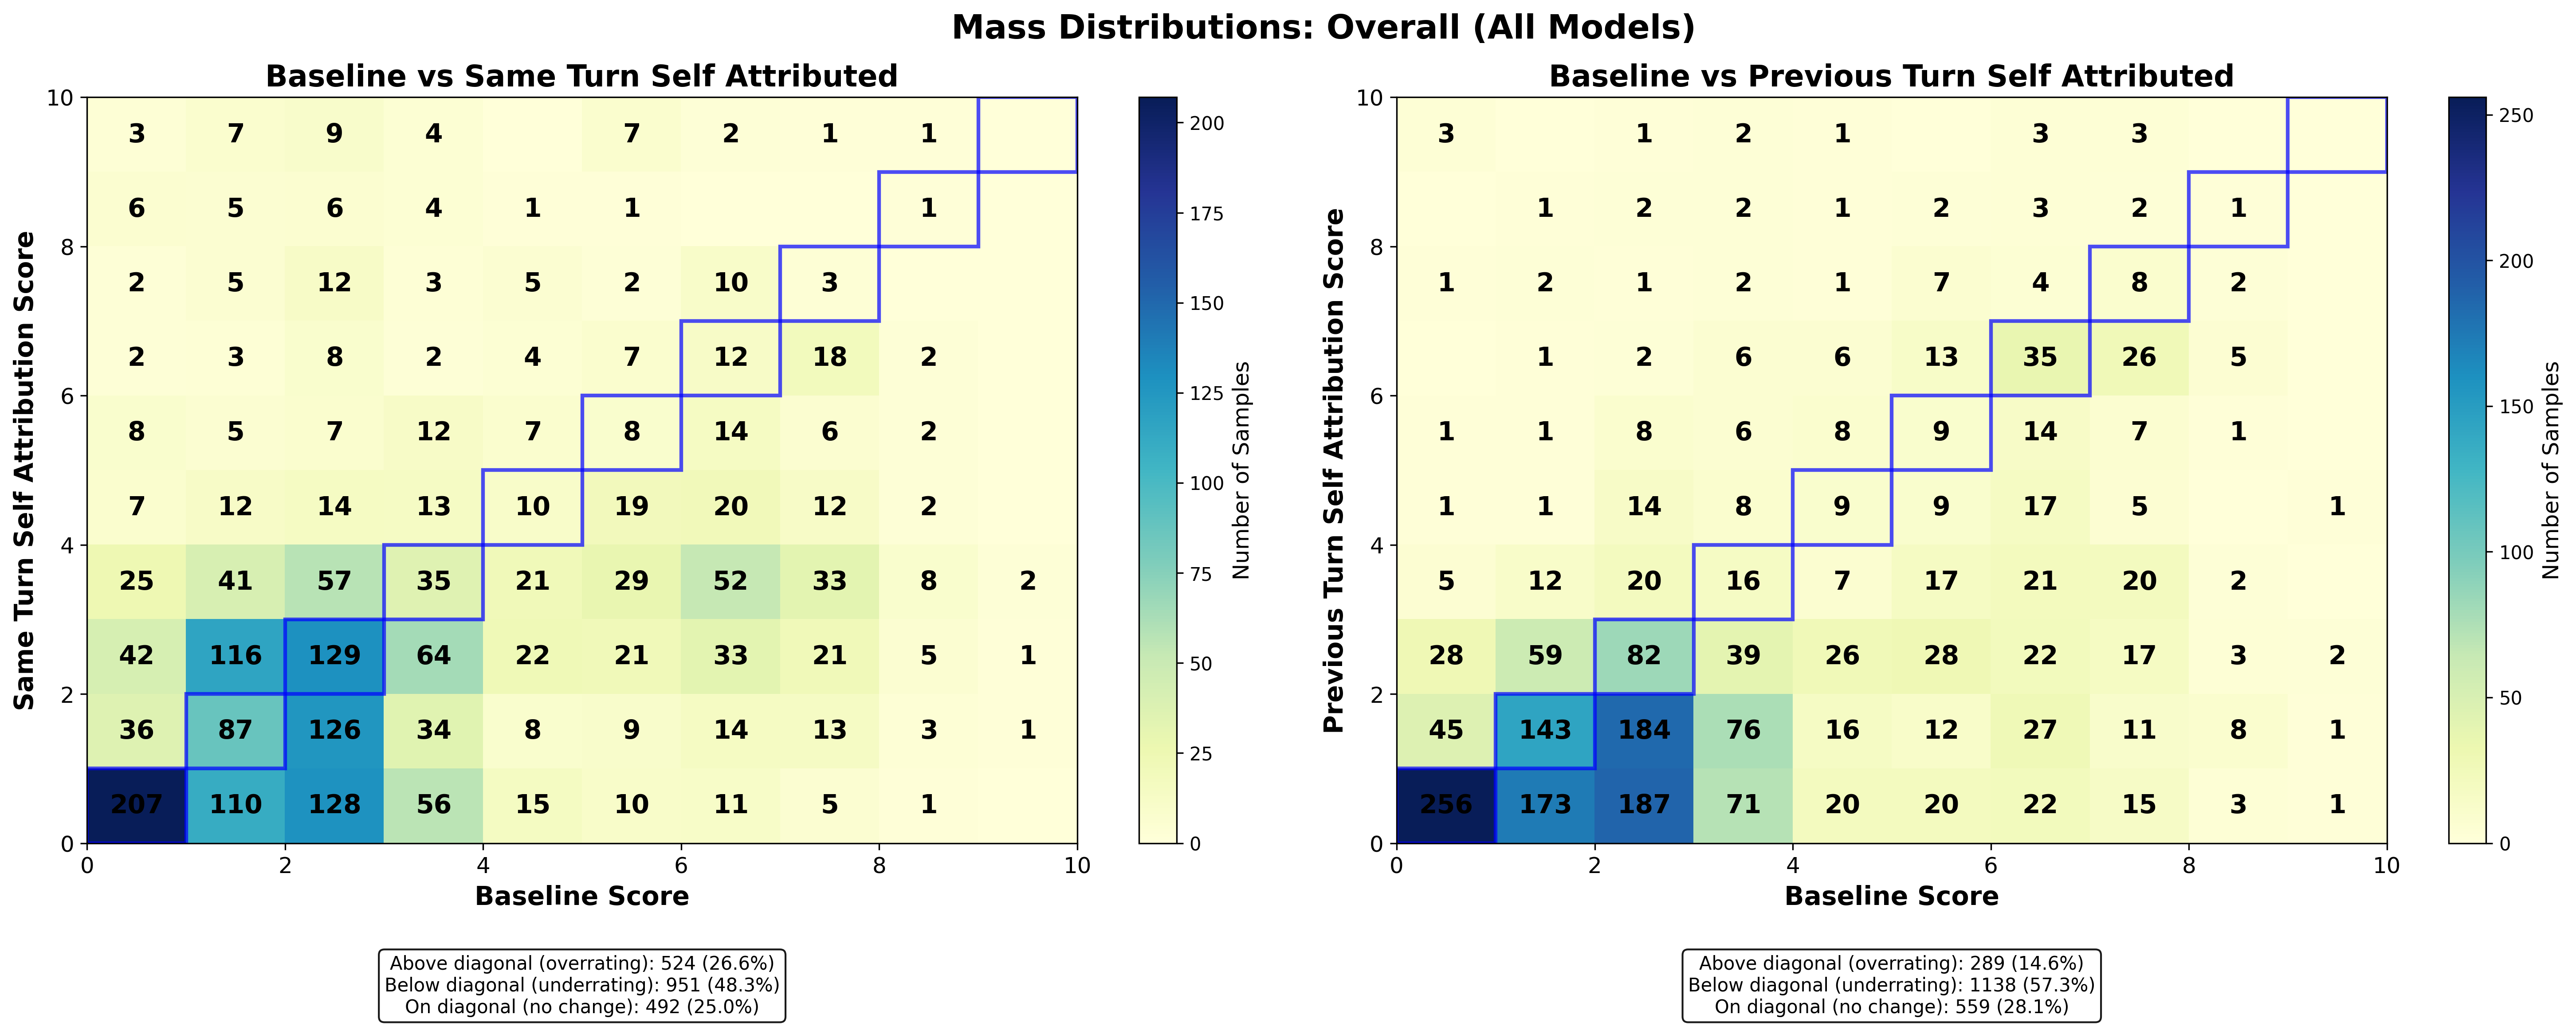
\includegraphics[width=\linewidth]{figures/mass_harmful_openended/mass_distributions_overall.png}
  \caption{Aggregate mass distribution of baseline vs.\ self-attributed ratings on Reddit ethical questions. Columns represent baseline bins; each column sums to 1 (conditional mass).}
  \label{fig:mass_overall}
\end{figure}

% Per-model mass distributions using ContinuedFloat
\begin{figure}[!tb]
  \centering
  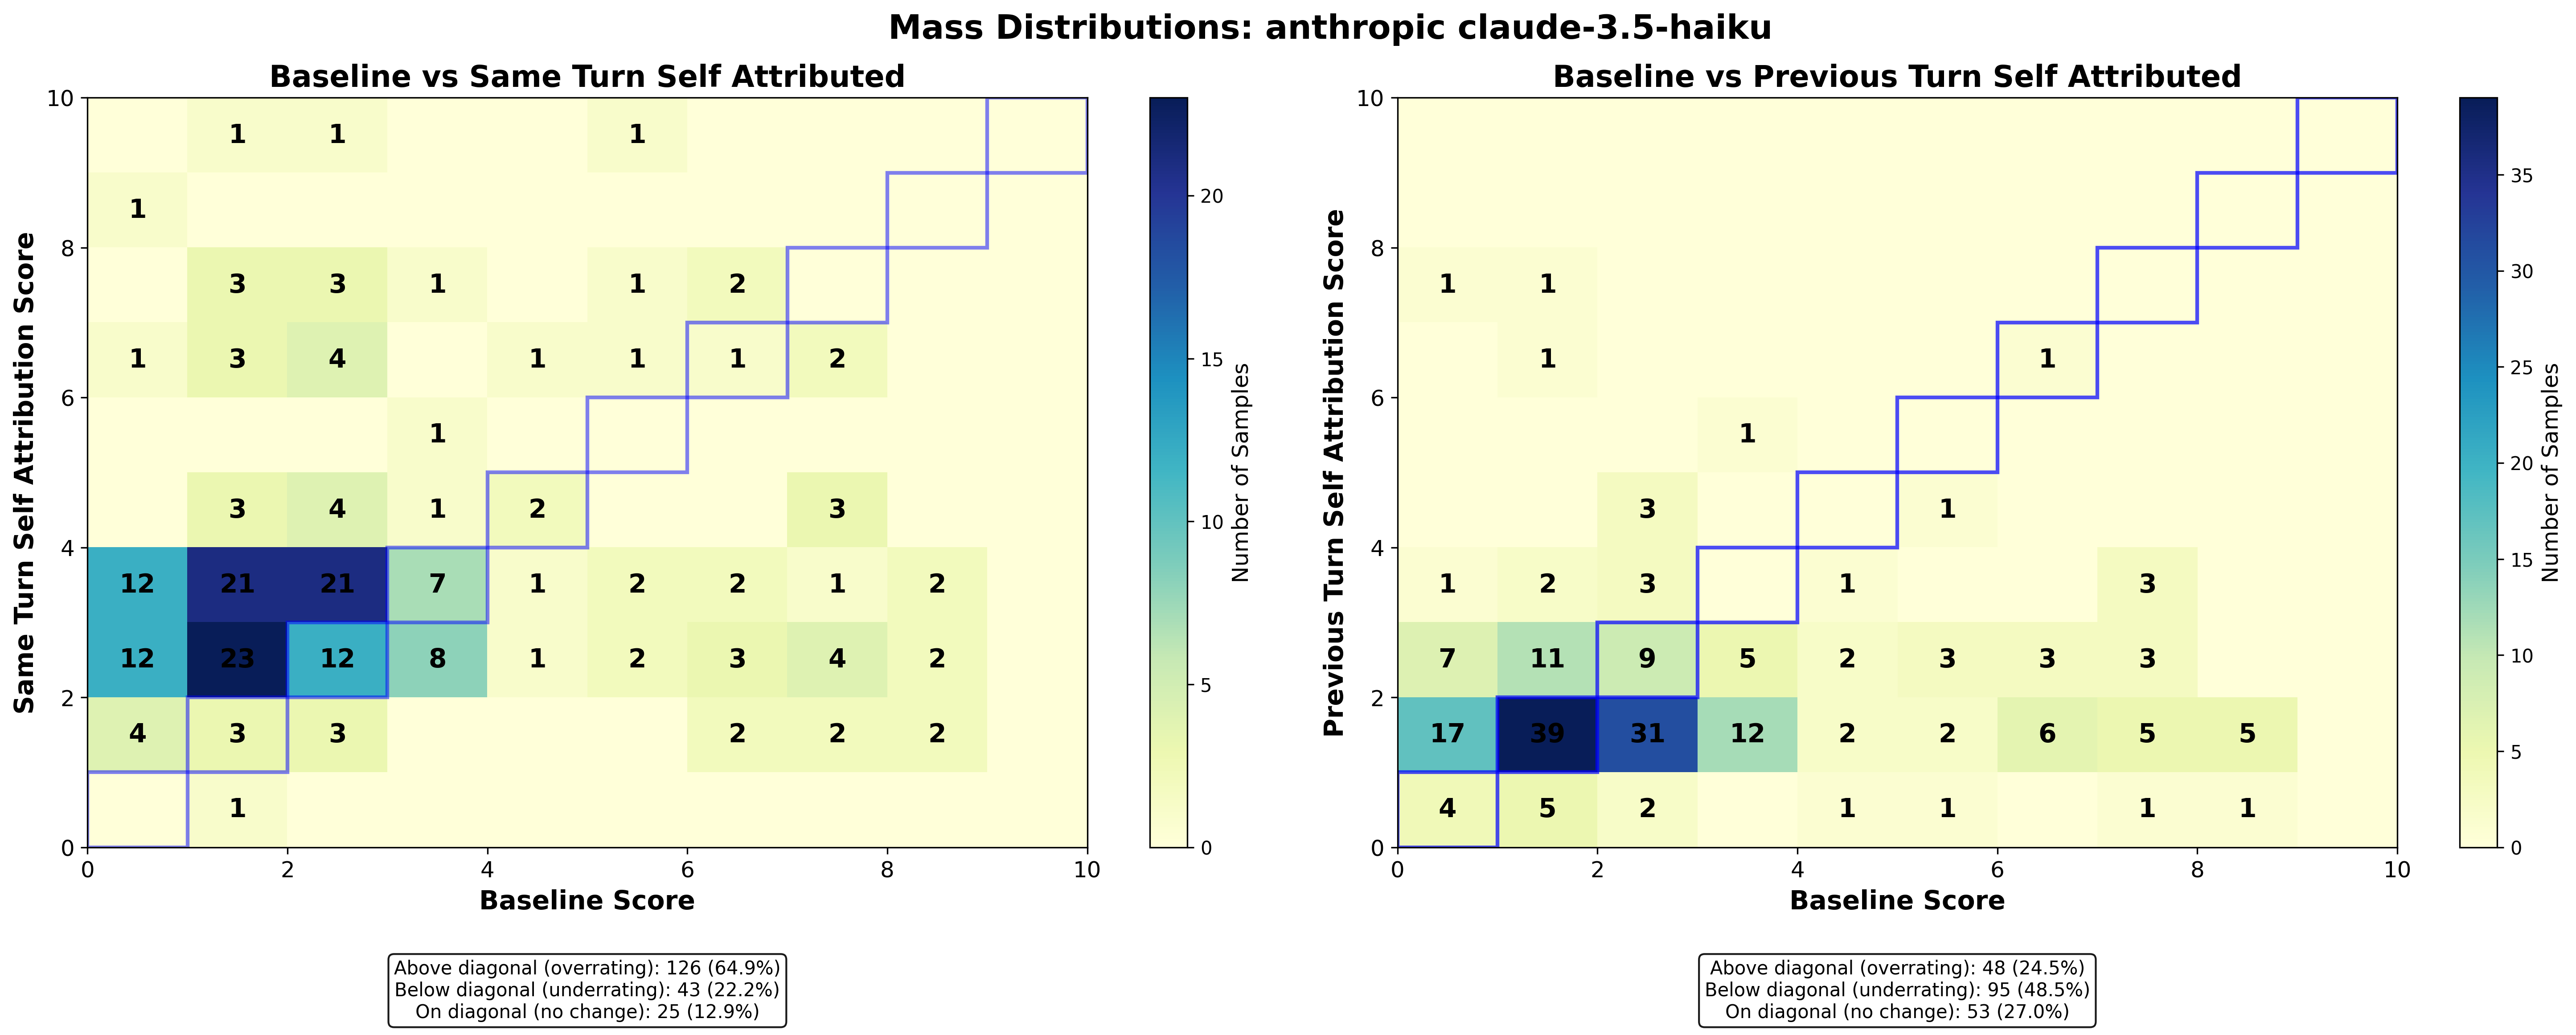
\includegraphics[width=\linewidth]{figures/mass_harmful_openended/mass_distributions_openrouter_anthropic_claude-3.5-haiku.png}
  \caption{Per-model mass distributions (baseline vs.\ self-attributed). Each column is normalized within a baseline bin. (a) Claude 3.5 Haiku.}
  \label{fig:mass_by_model}
\end{figure}

\begin{figure}[!tb]
  \ContinuedFloat
  \centering
  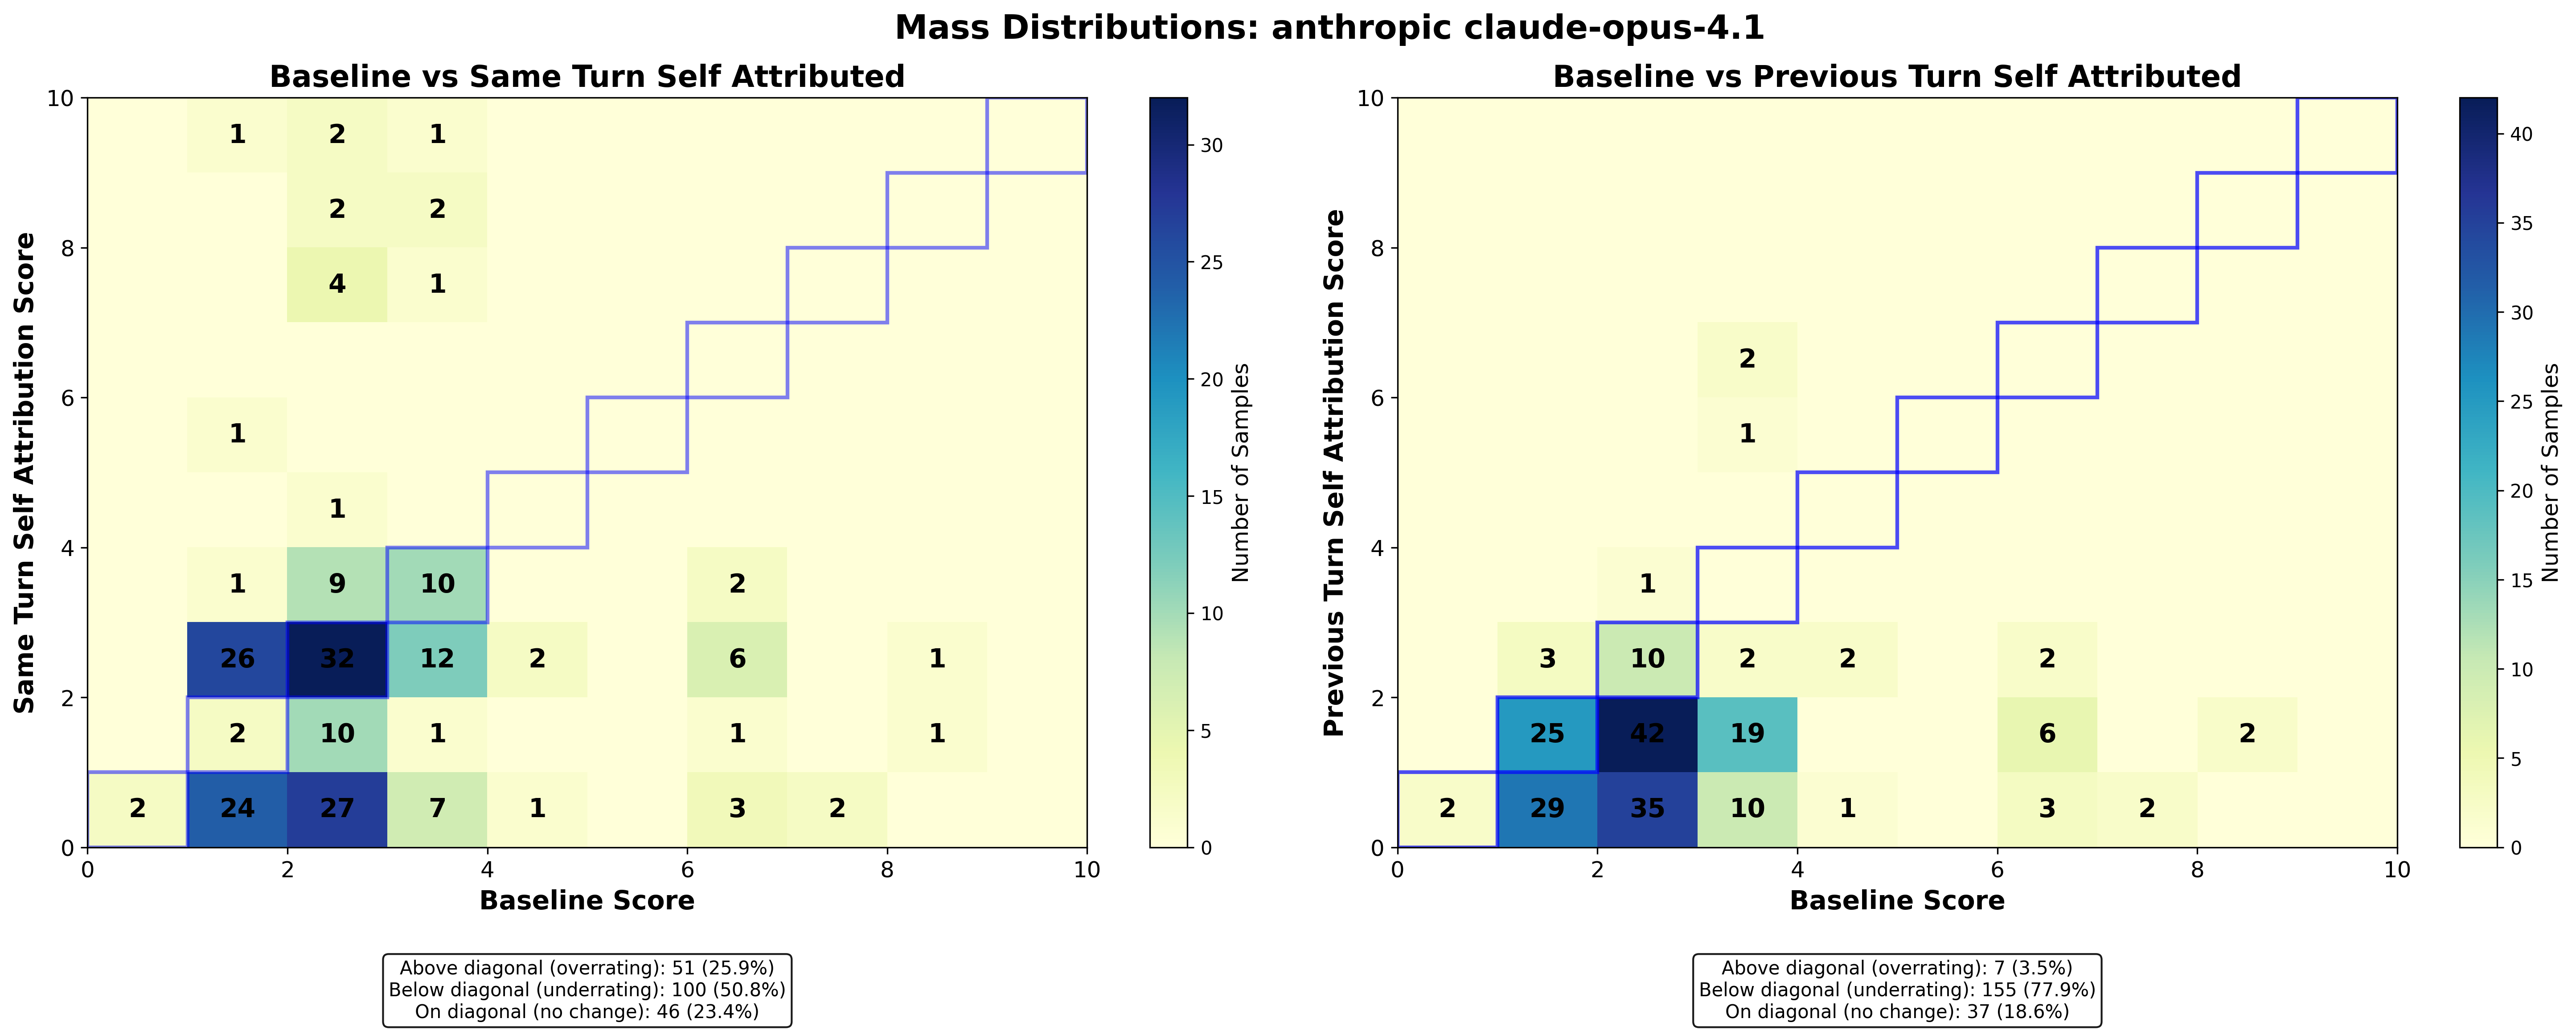
\includegraphics[width=\linewidth]{figures/mass_harmful_openended/mass_distributions_openrouter_anthropic_claude-opus-4.1.png}
  \caption{(cont.) (b) Claude 4.1 Opus.}
\end{figure}

\begin{figure}[!tb]
  \ContinuedFloat
  \centering
  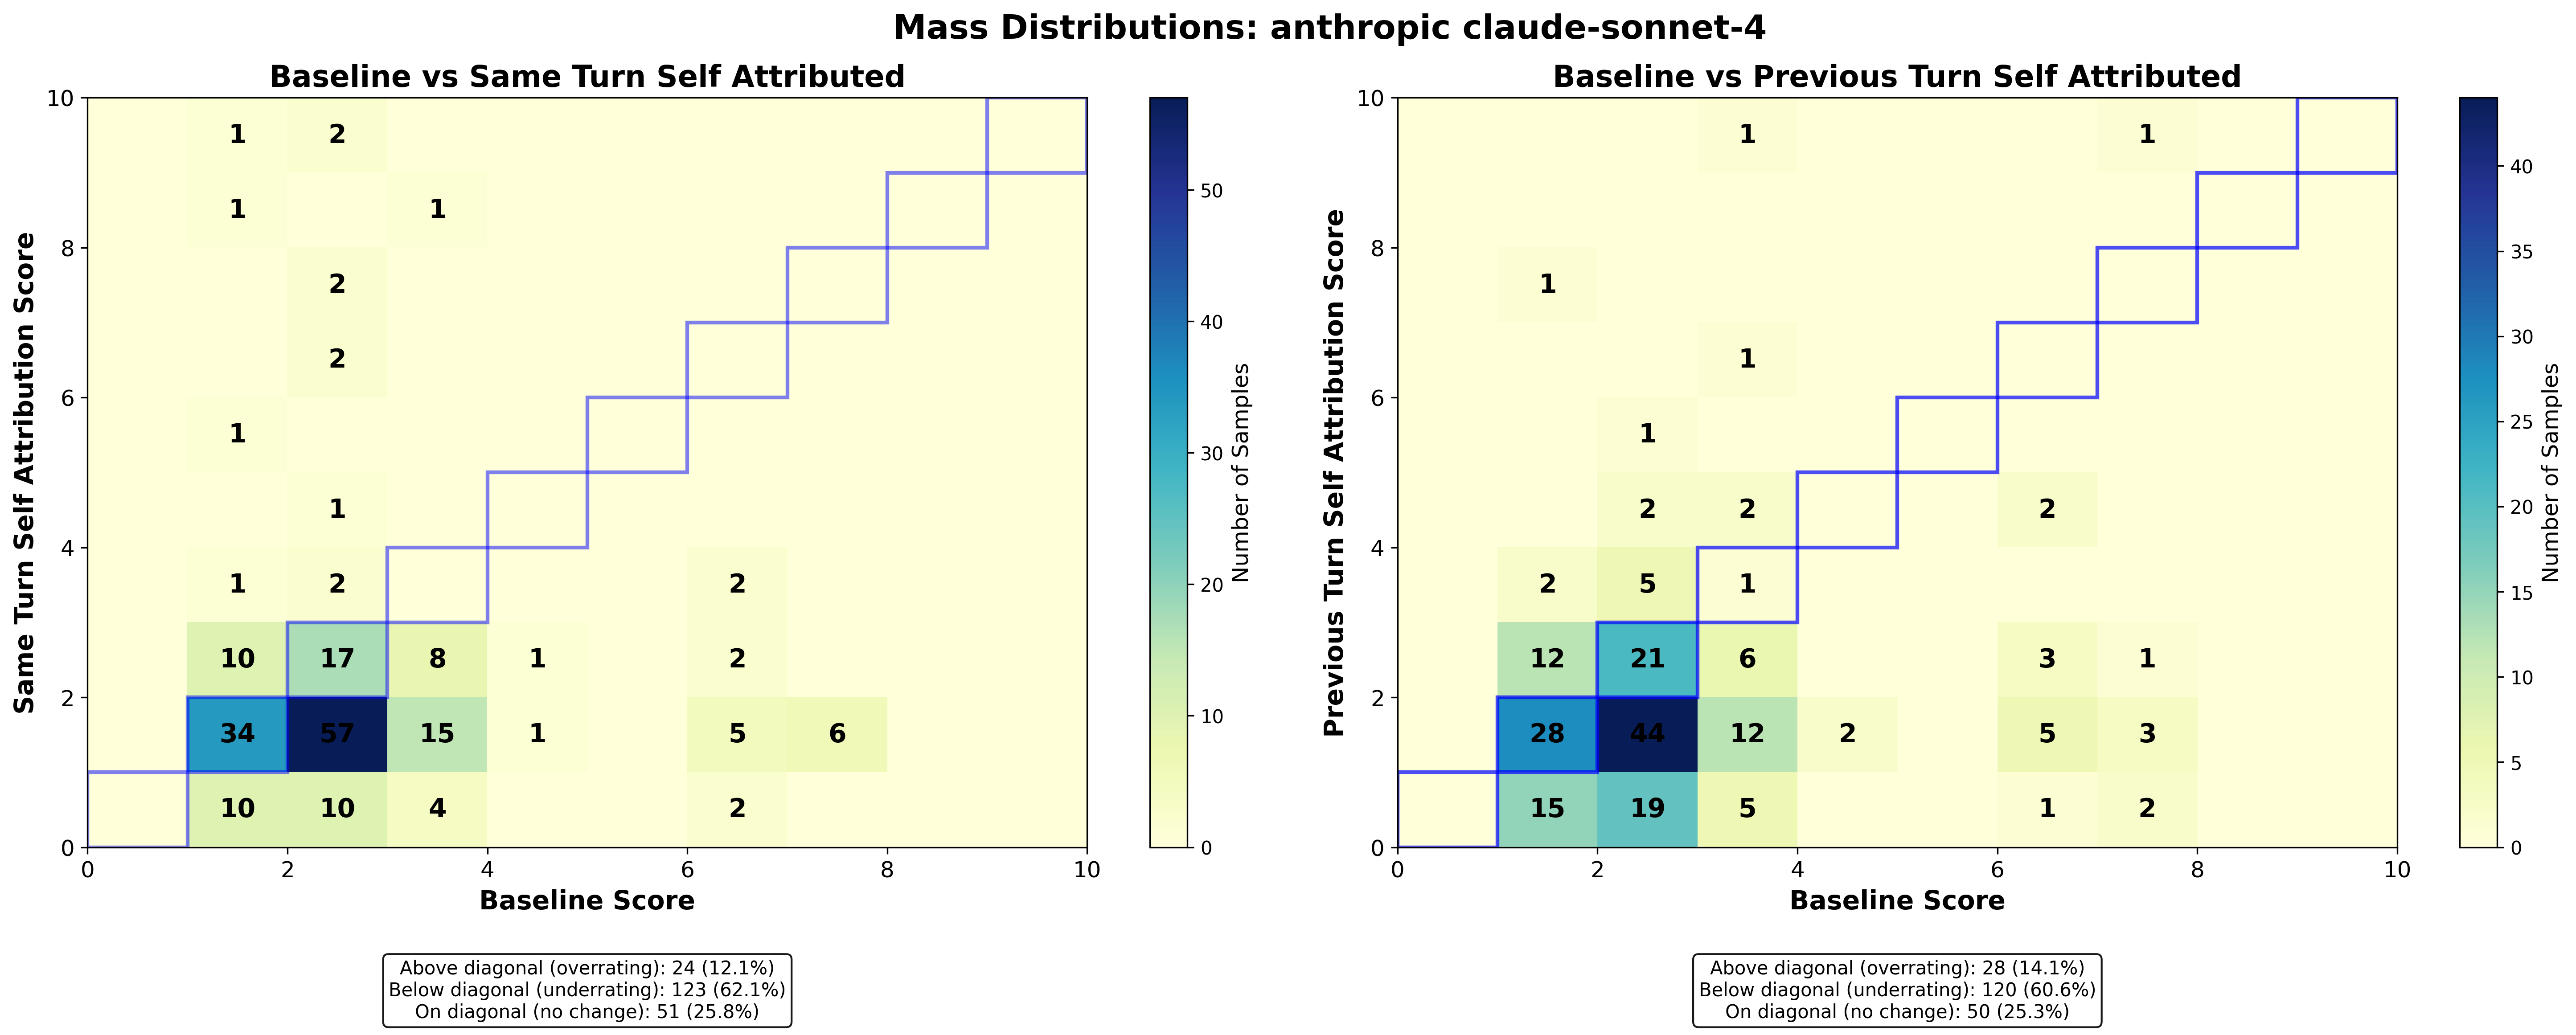
\includegraphics[width=\linewidth]{figures/mass_harmful_openended/mass_distributions_openrouter_anthropic_claude-sonnet-4.png}
  \caption{(cont.) (c) Claude 4 Sonnet.}
\end{figure}

\begin{figure}[!tb]
  \ContinuedFloat
  \centering
  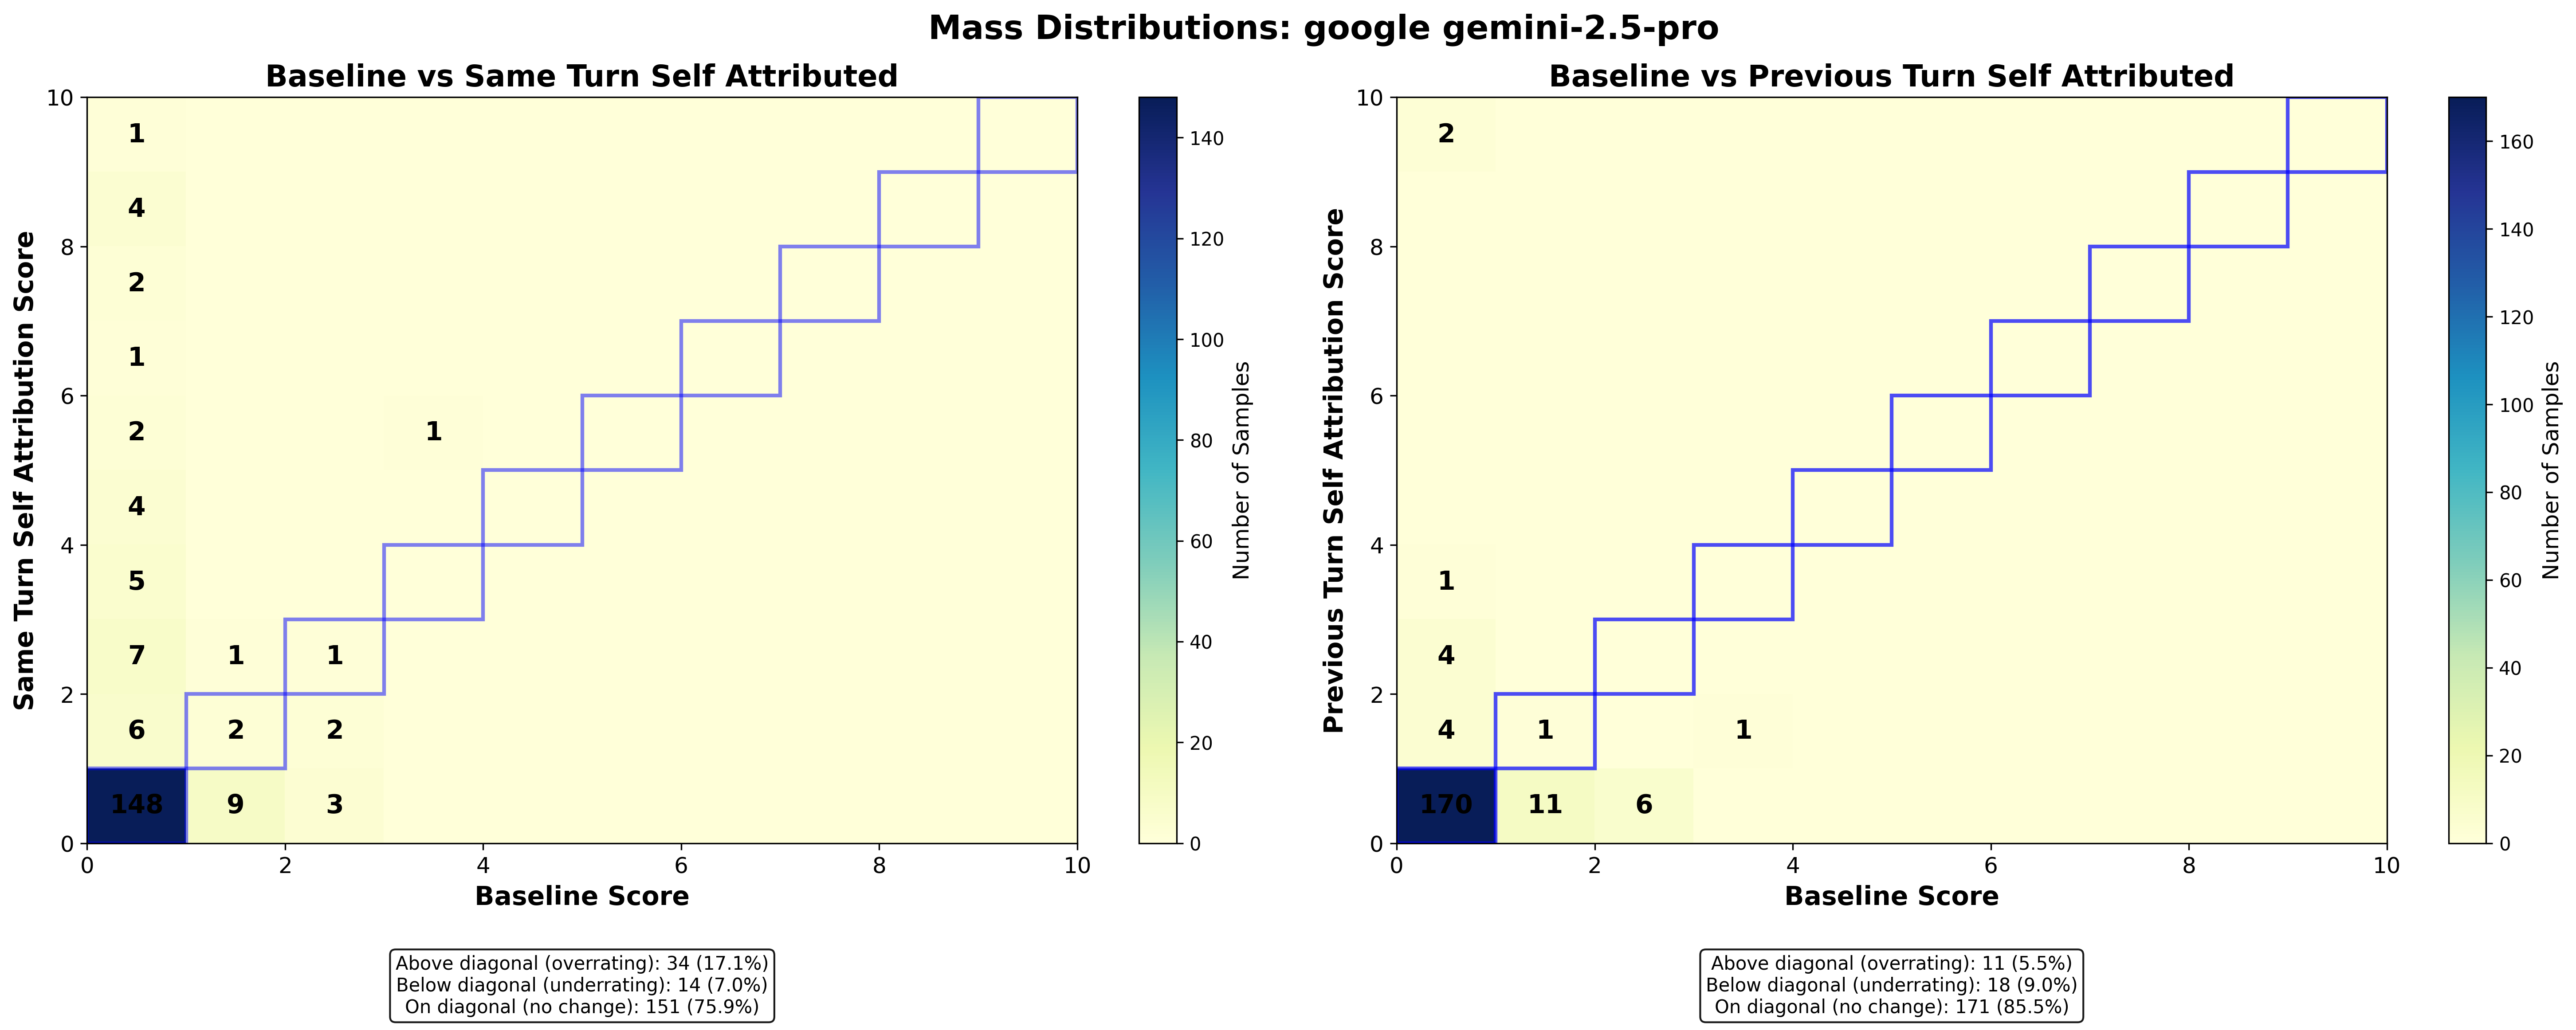
\includegraphics[width=\linewidth]{figures/mass_harmful_openended/mass_distributions_openrouter_google_gemini-2.5-pro.png}
  \caption{(cont.) (d) Gemini 2.5 Pro.}
\end{figure}

\begin{figure}[!tb]
  \ContinuedFloat
  \centering
  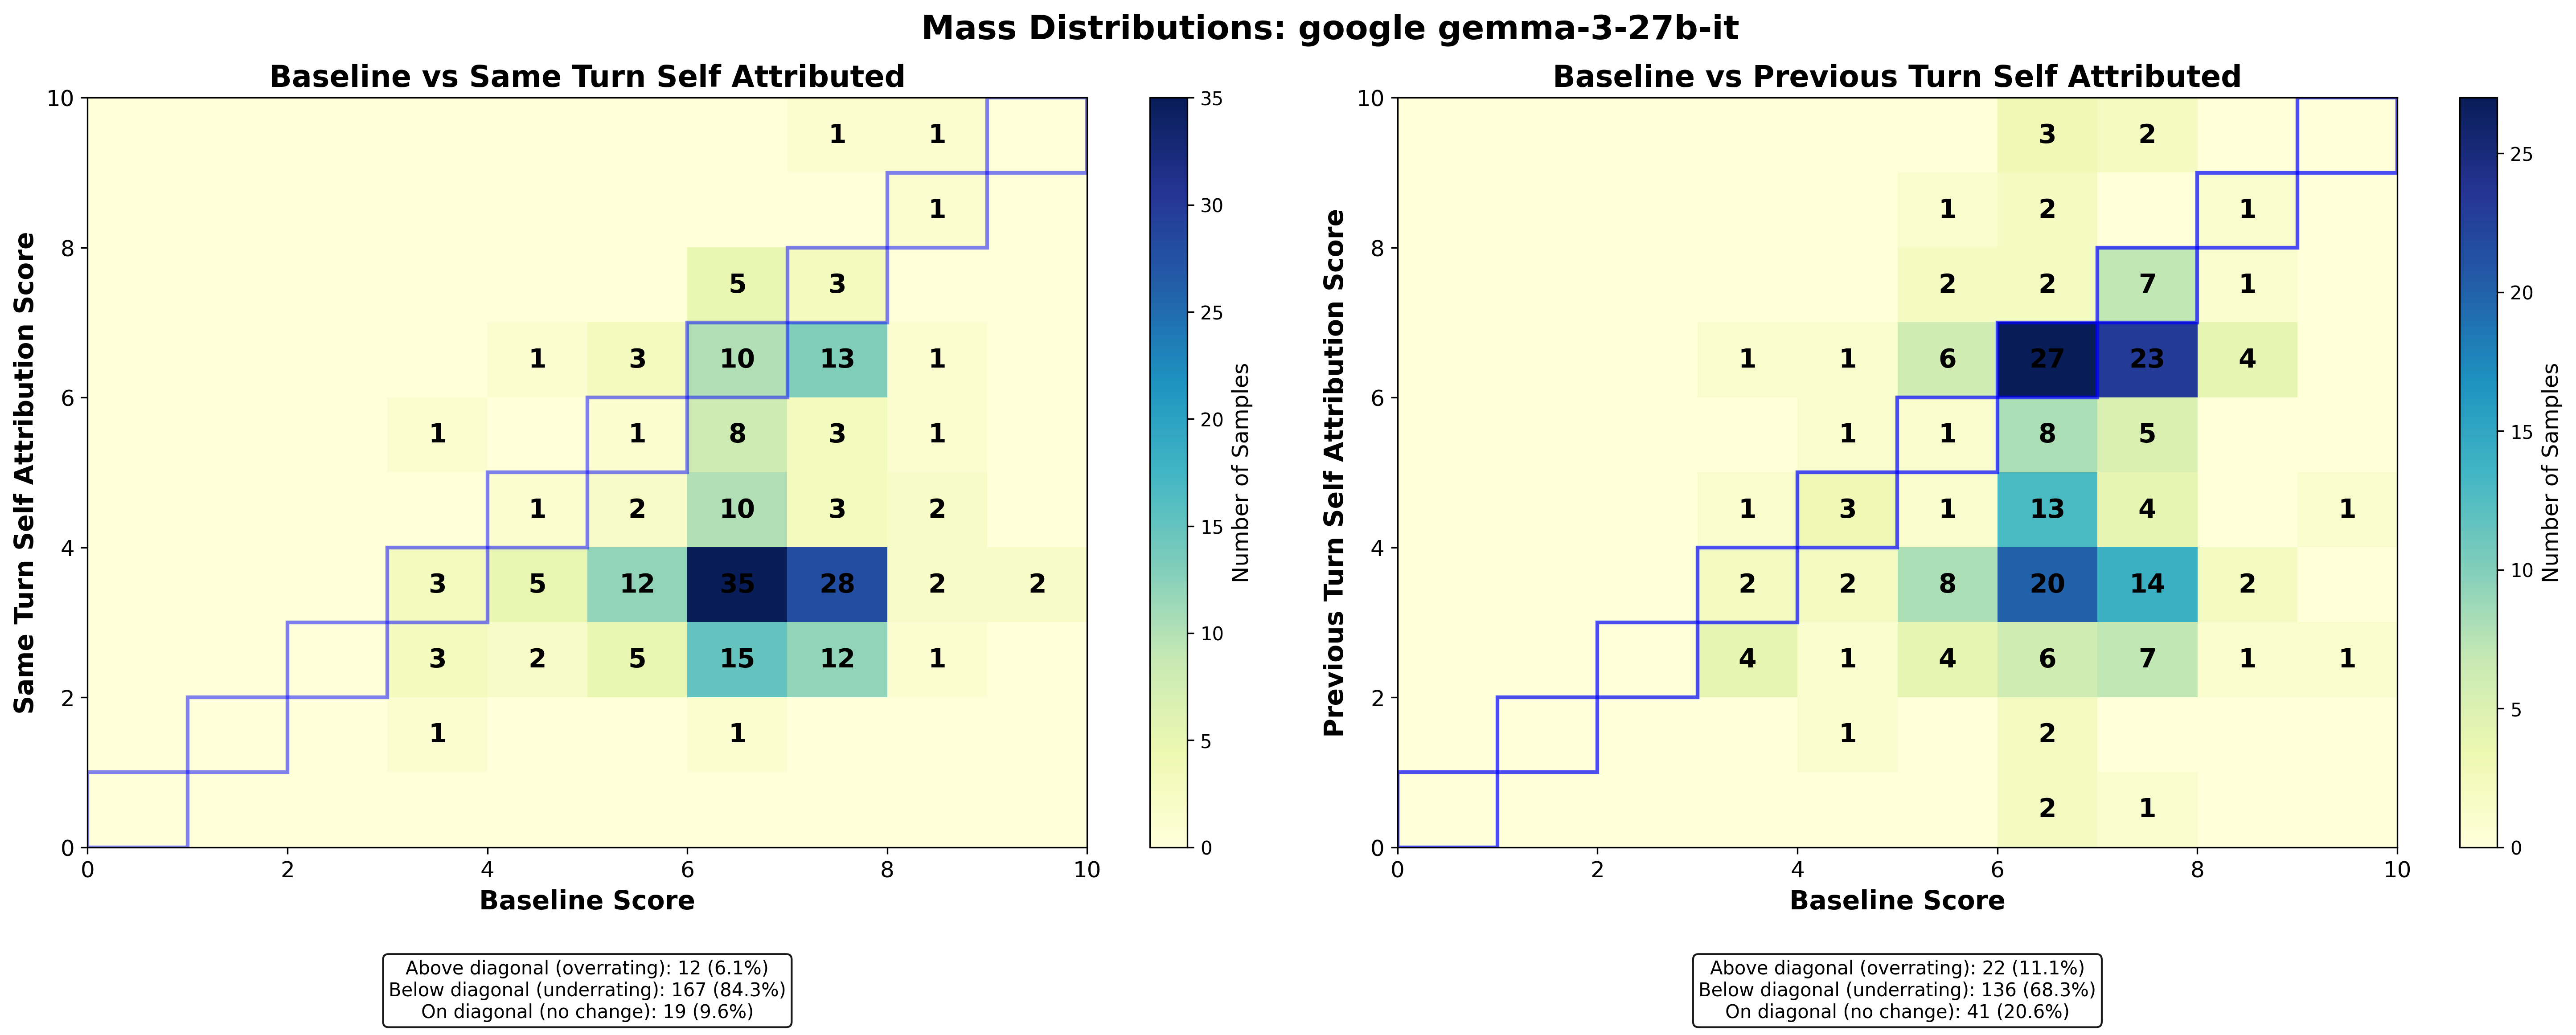
\includegraphics[width=\linewidth]{figures/mass_harmful_openended/mass_distributions_openrouter_google_gemma-3-27b-it.png}
  \caption{(cont.) (e) Gemma-3 27B-IT.}
\end{figure}

\begin{figure}[!tb]
  \ContinuedFloat
  \centering
  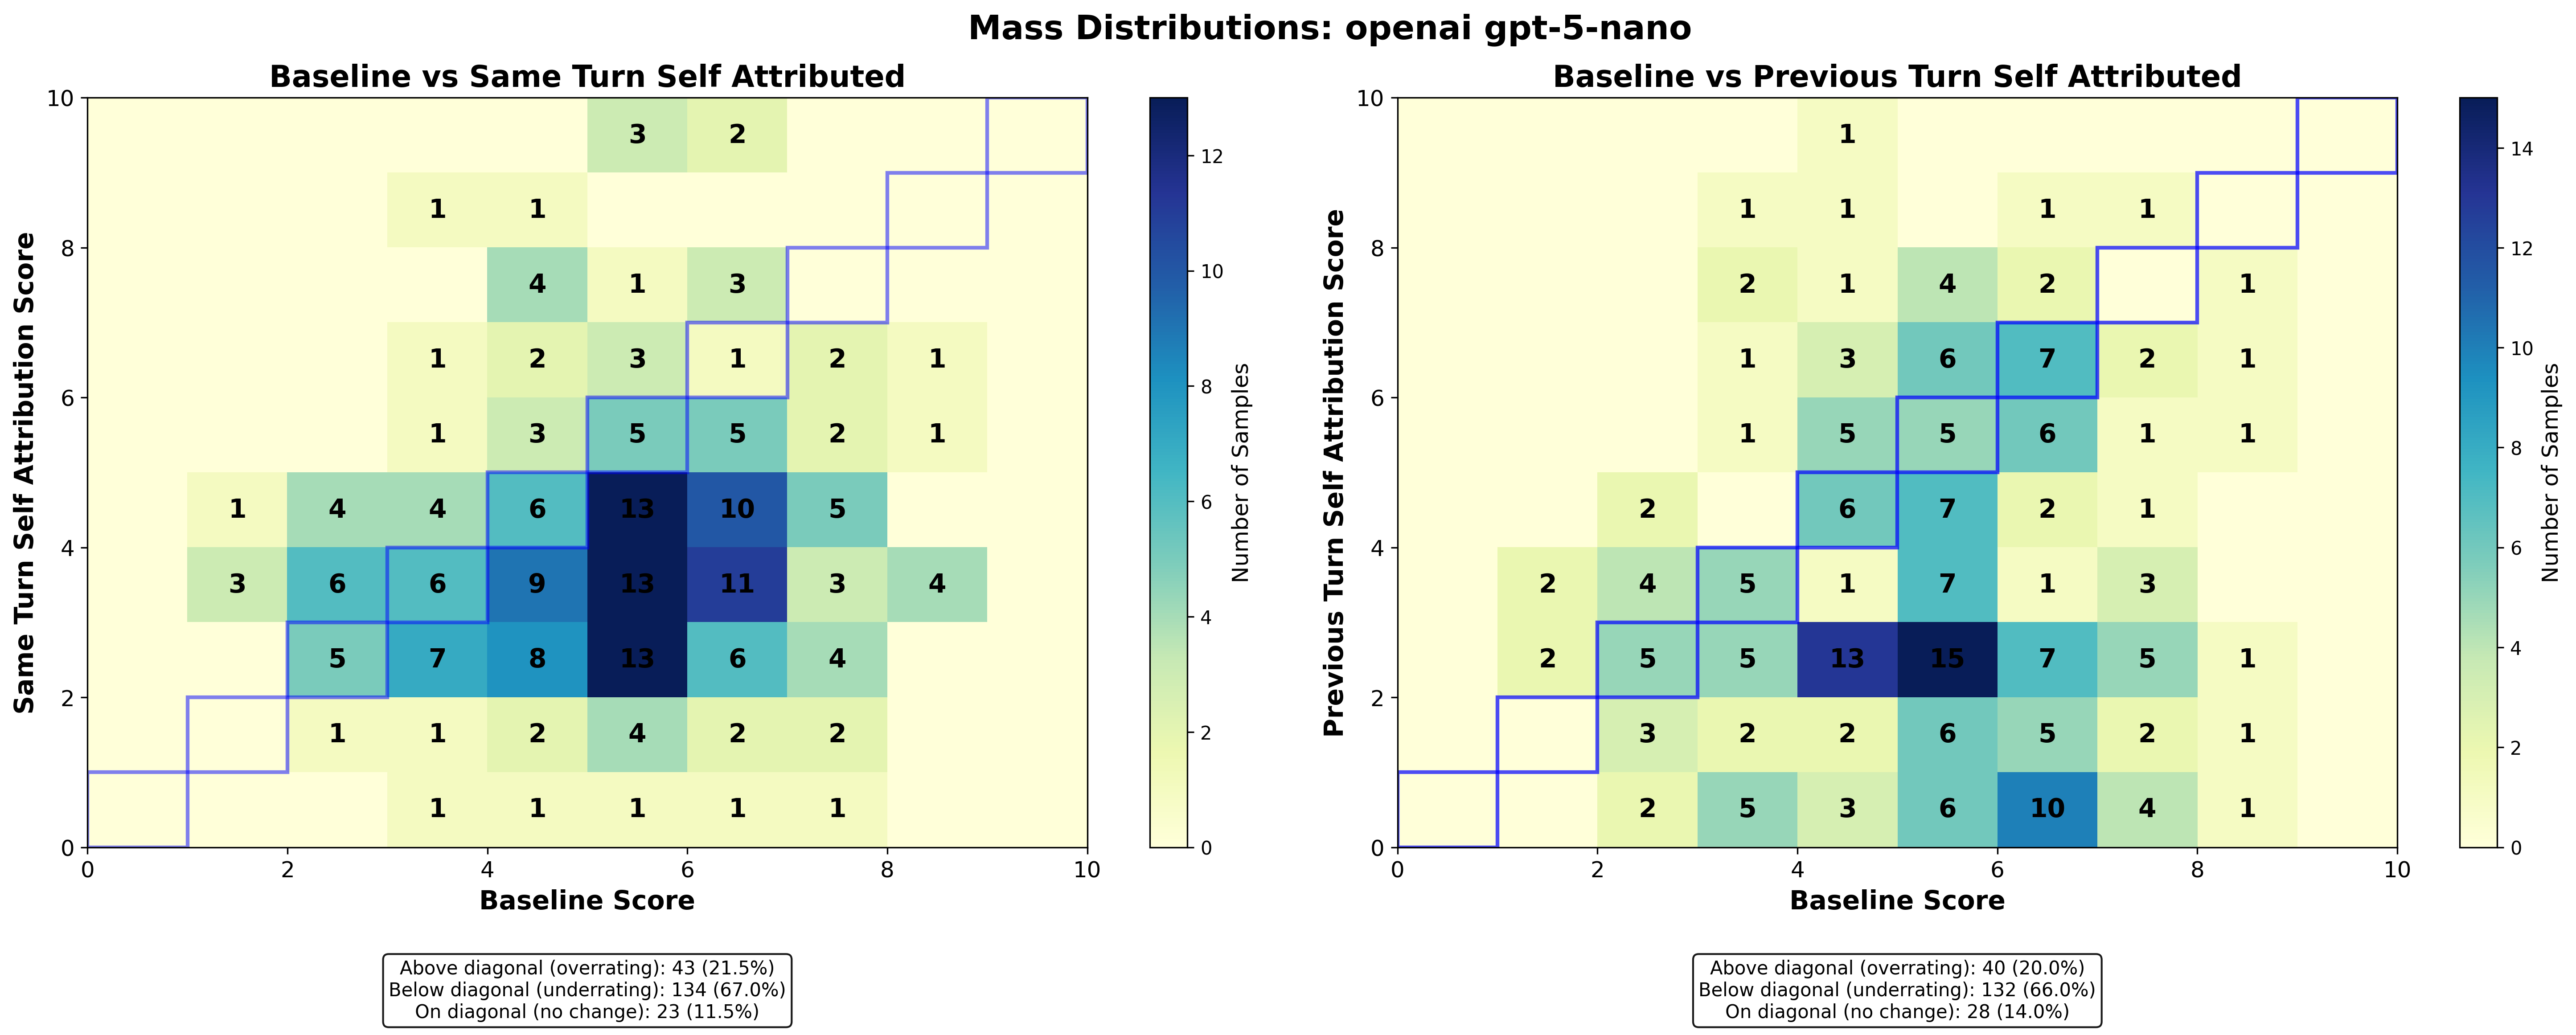
\includegraphics[width=\linewidth]{figures/mass_harmful_openended/mass_distributions_openrouter_openai_gpt-5-nano.png}
  \caption{(cont.) (f) GPT-5 Nano.}
\end{figure}

\begin{figure}[!tb]
  \ContinuedFloat
  \centering
  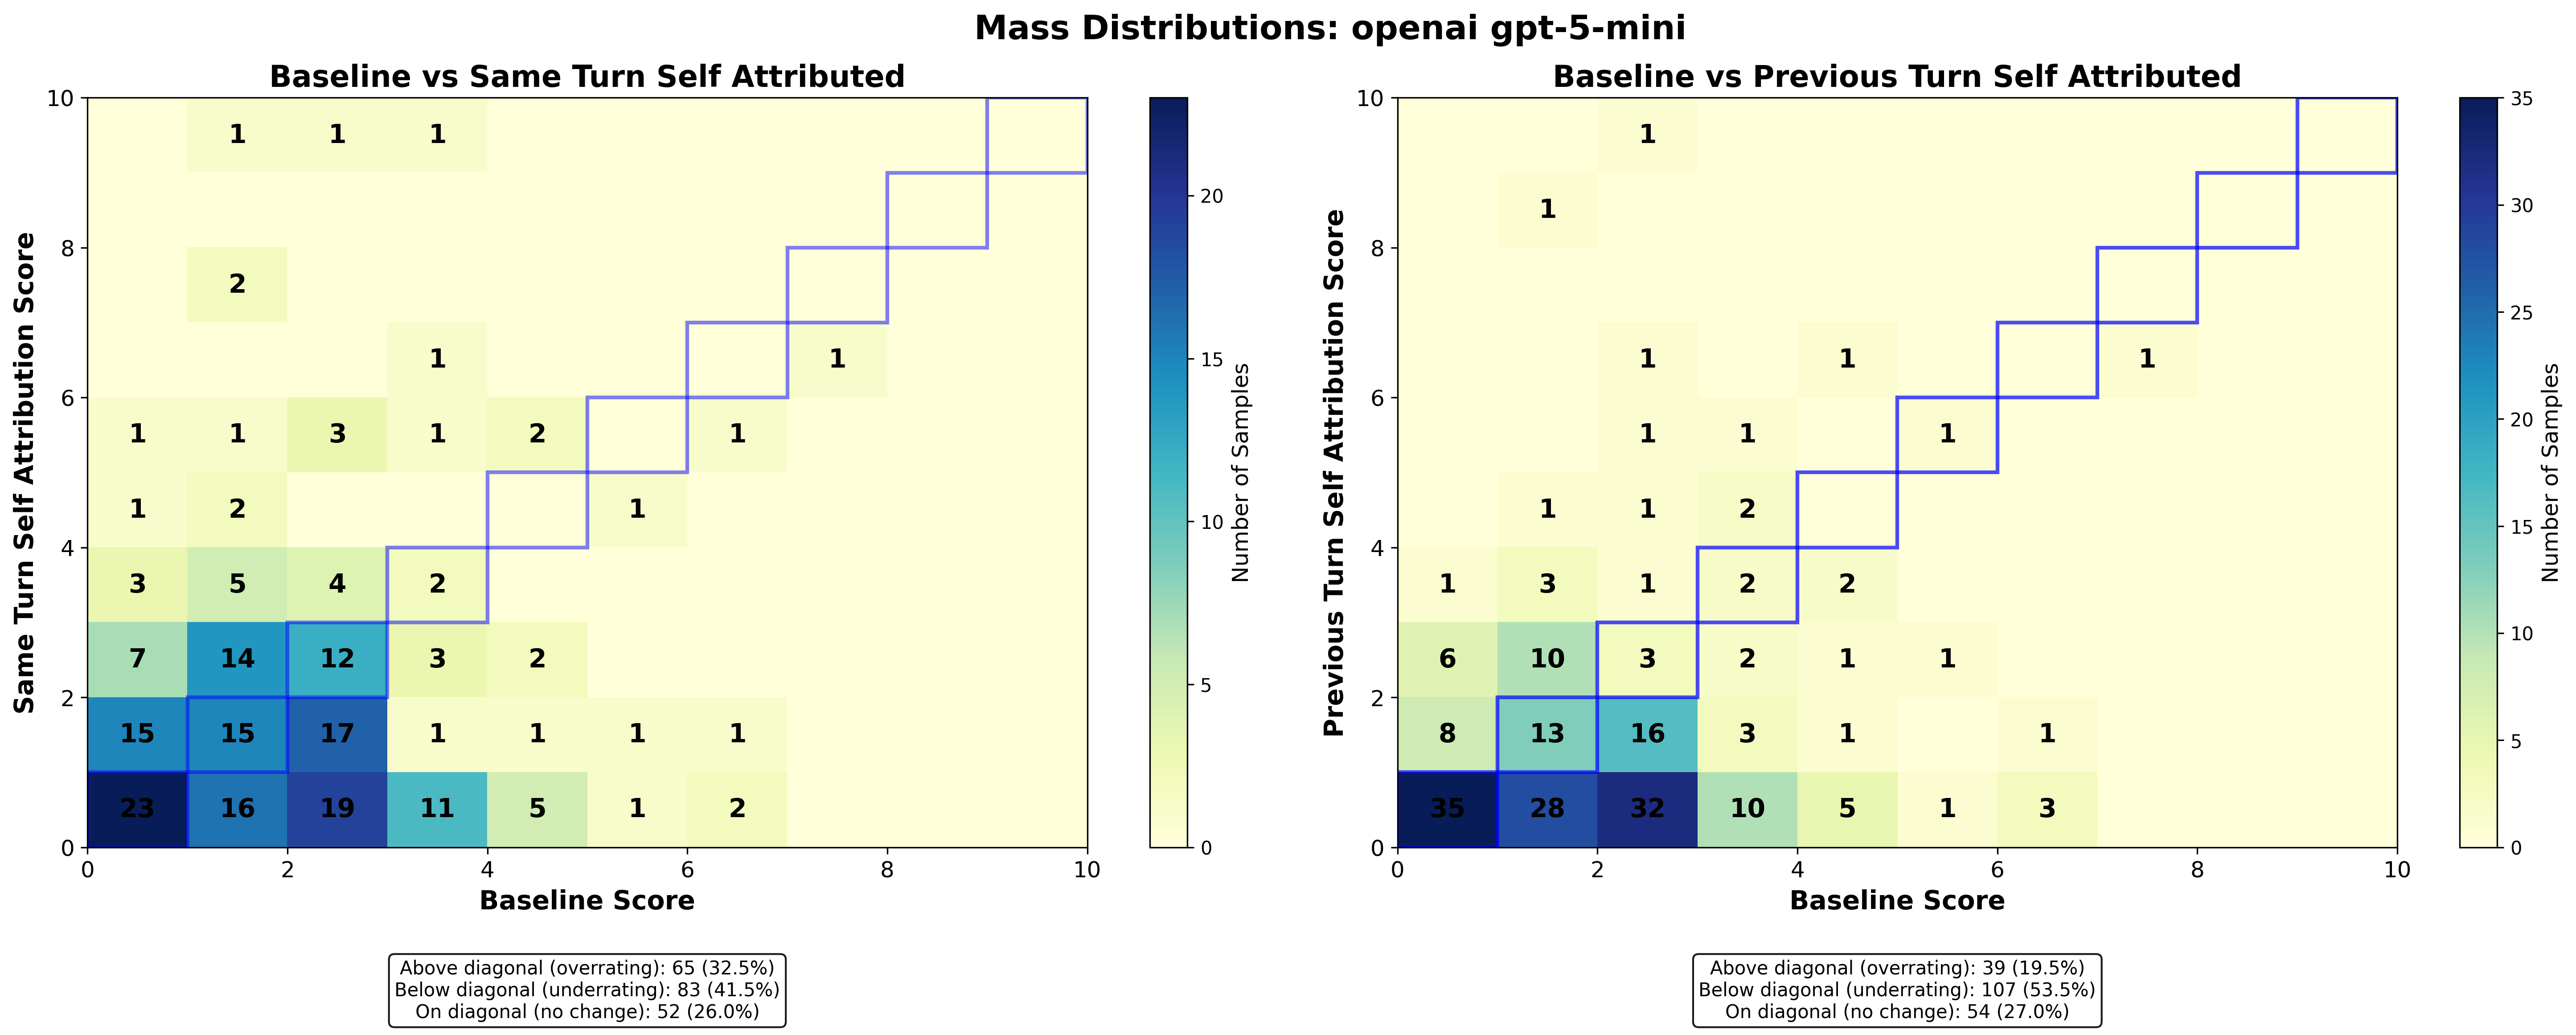
\includegraphics[width=\linewidth]{figures/mass_harmful_openended/mass_distributions_openrouter_openai_gpt-5-mini.png}
  \caption{(cont.) (g) GPT-5 Mini.}
\end{figure}

\begin{figure}[!tb]
  \ContinuedFloat
  \centering
  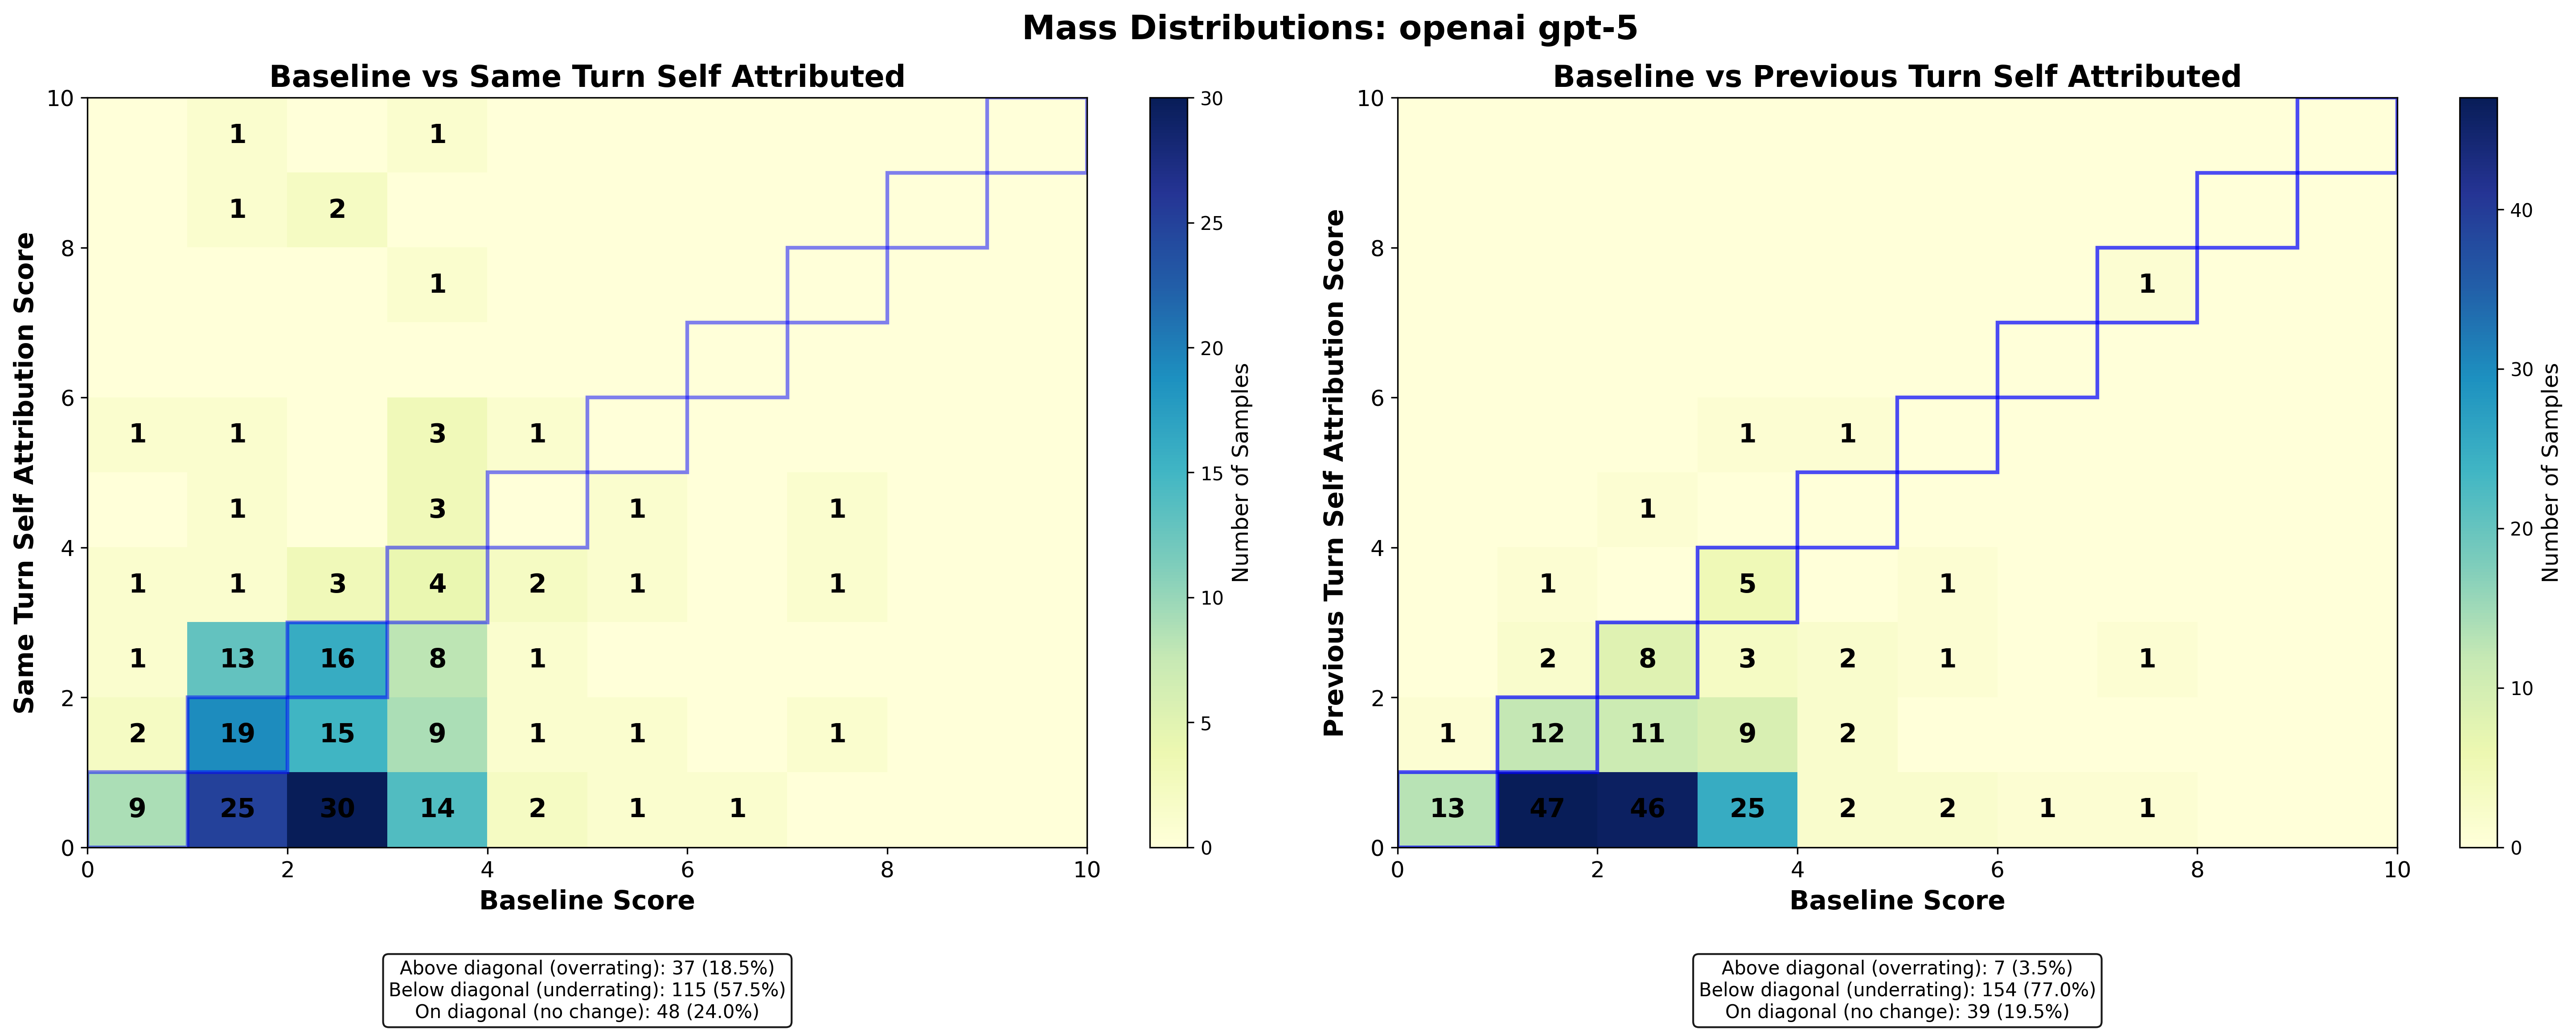
\includegraphics[width=\linewidth]{figures/mass_harmful_openended/mass_distributions_openrouter_openai_gpt-5.png}
  \caption{(cont.) (h) GPT-5.}
\end{figure}

\begin{figure}[!tb]
  \ContinuedFloat
  \centering
  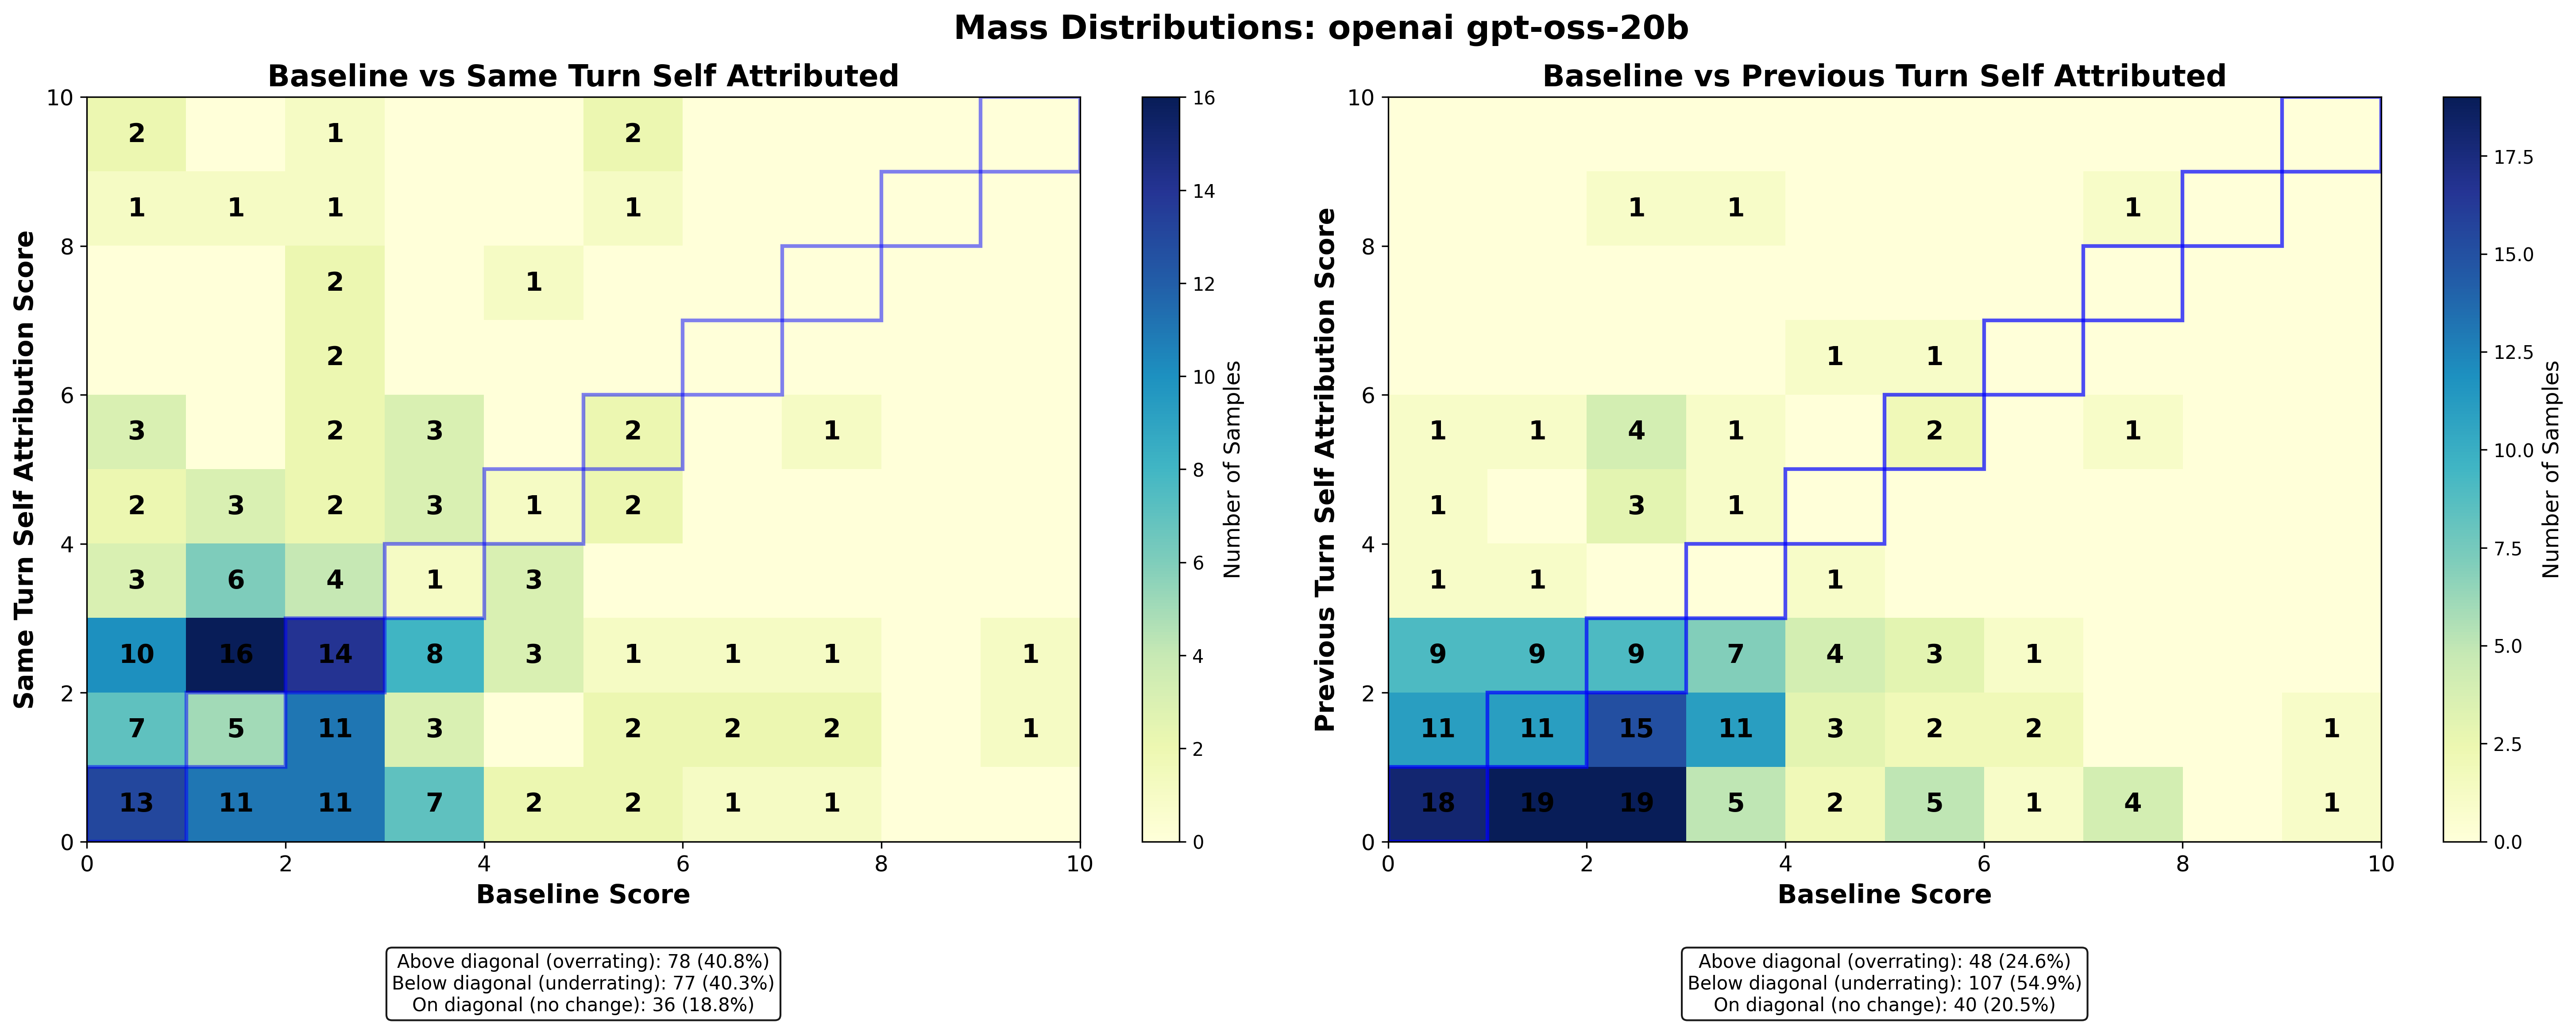
\includegraphics[width=\linewidth]{figures/mass_harmful_openended/mass_distributions_openrouter_openai_gpt-oss-20b.png}
  \caption{(cont.) (i) GPT-OSS-20B.}
\end{figure}

\begin{figure}[!tb]
  \ContinuedFloat
  \centering
  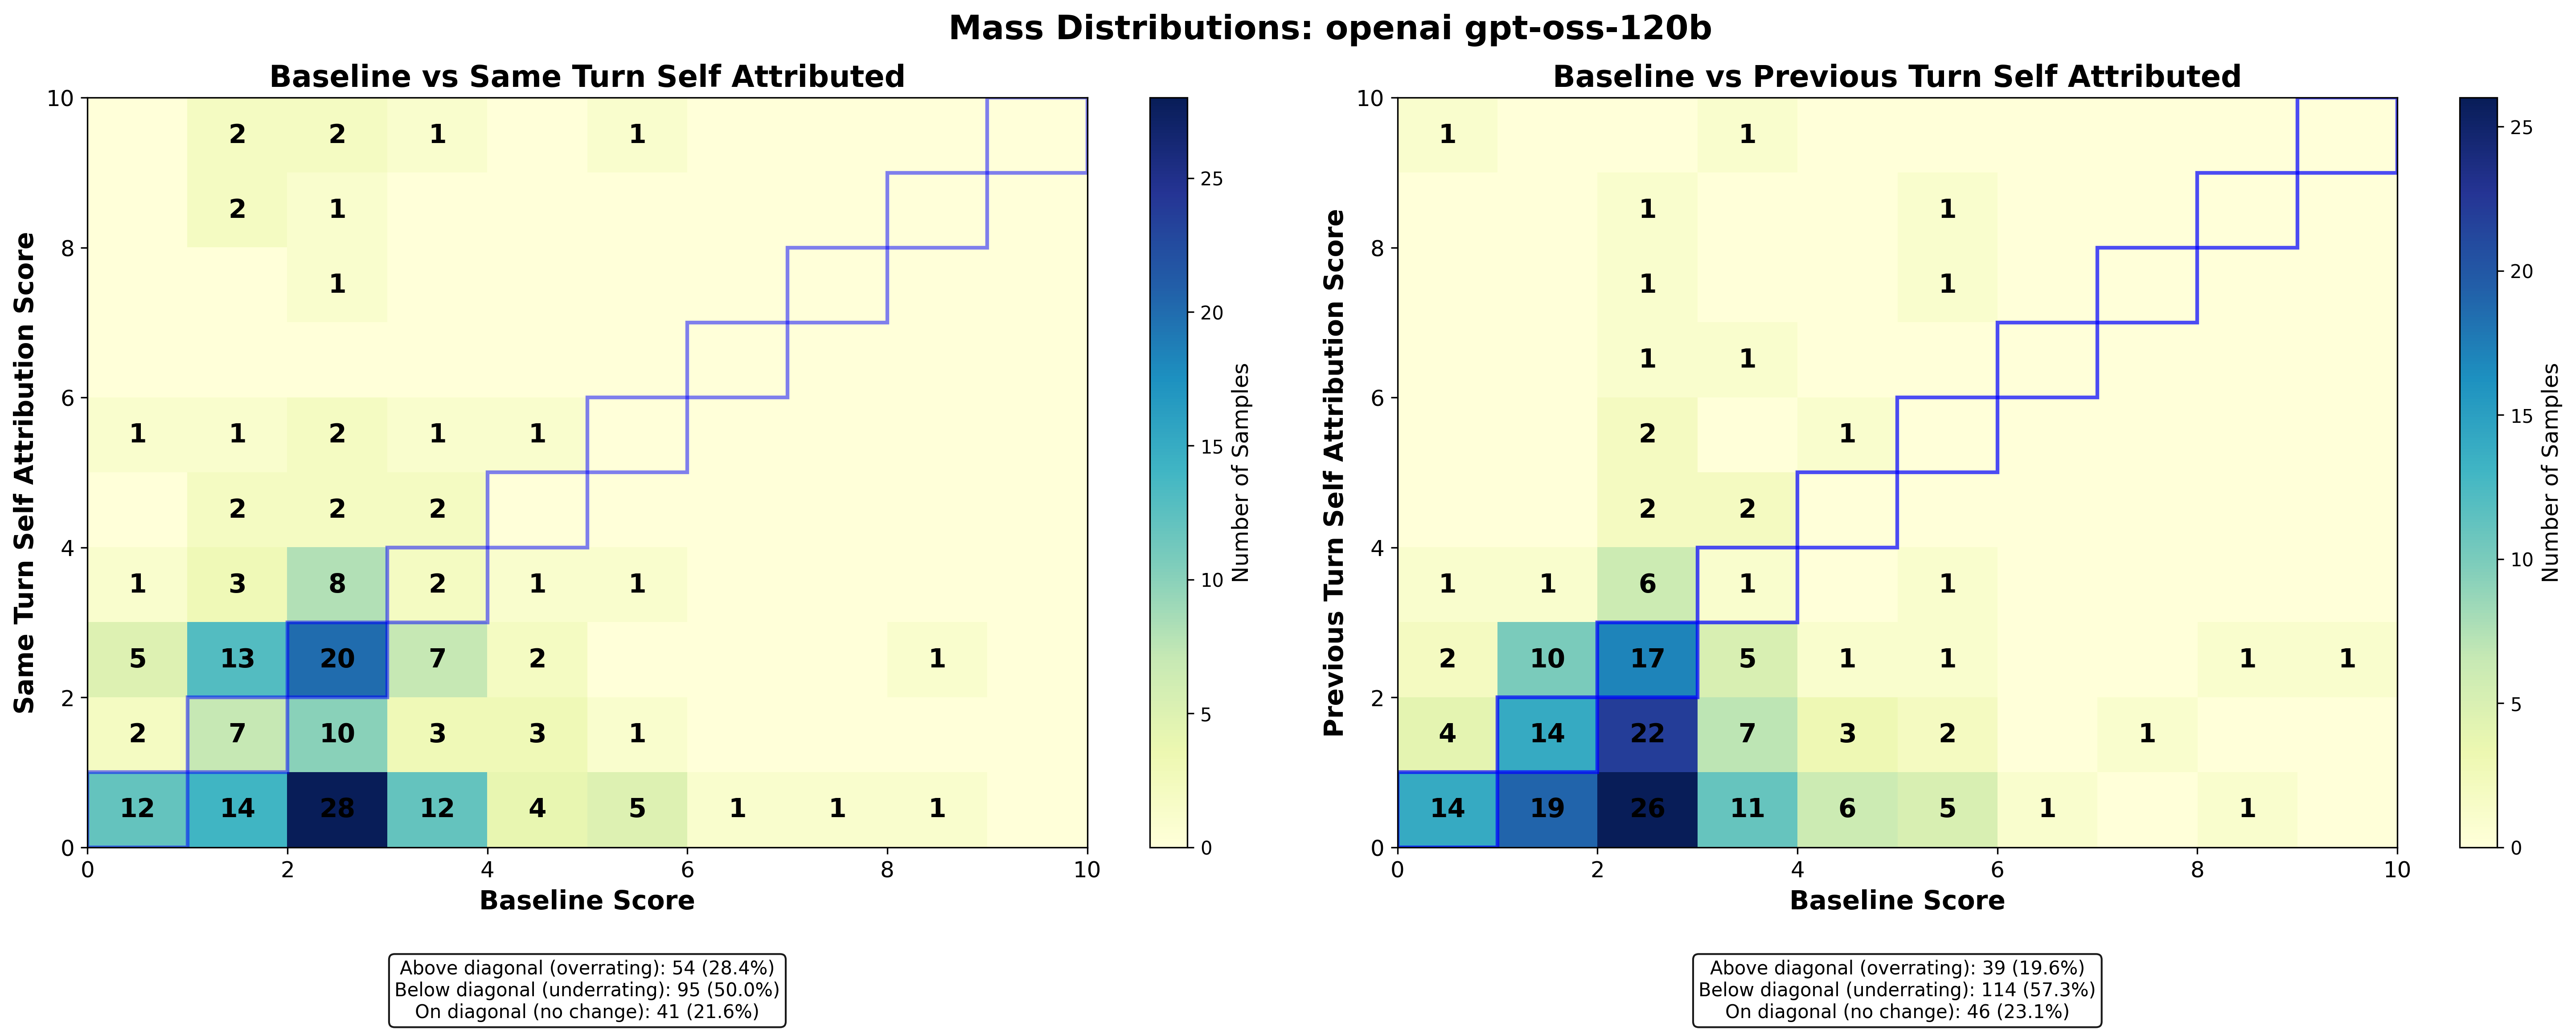
\includegraphics[width=\linewidth]{figures/mass_harmful_openended/mass_distributions_openrouter_openai_gpt-oss-120b.png}
  \caption{(cont.) (j) GPT-OSS-120B.}
\end{figure}

\FloatBarrier
\clearpage

%==============================================================================
\section{Per-Model Performance Summary}
\label{app:results:per-model-summary}
%==============================================================================

The following figures show individual model performance across harmfulness and correctness MCQ domains. Each panel shows pre-choice and post-choice scores with 95\% confidence intervals. $\Delta$ values denote mean score shifts.

\begin{figure}[!tb]
  \centering
  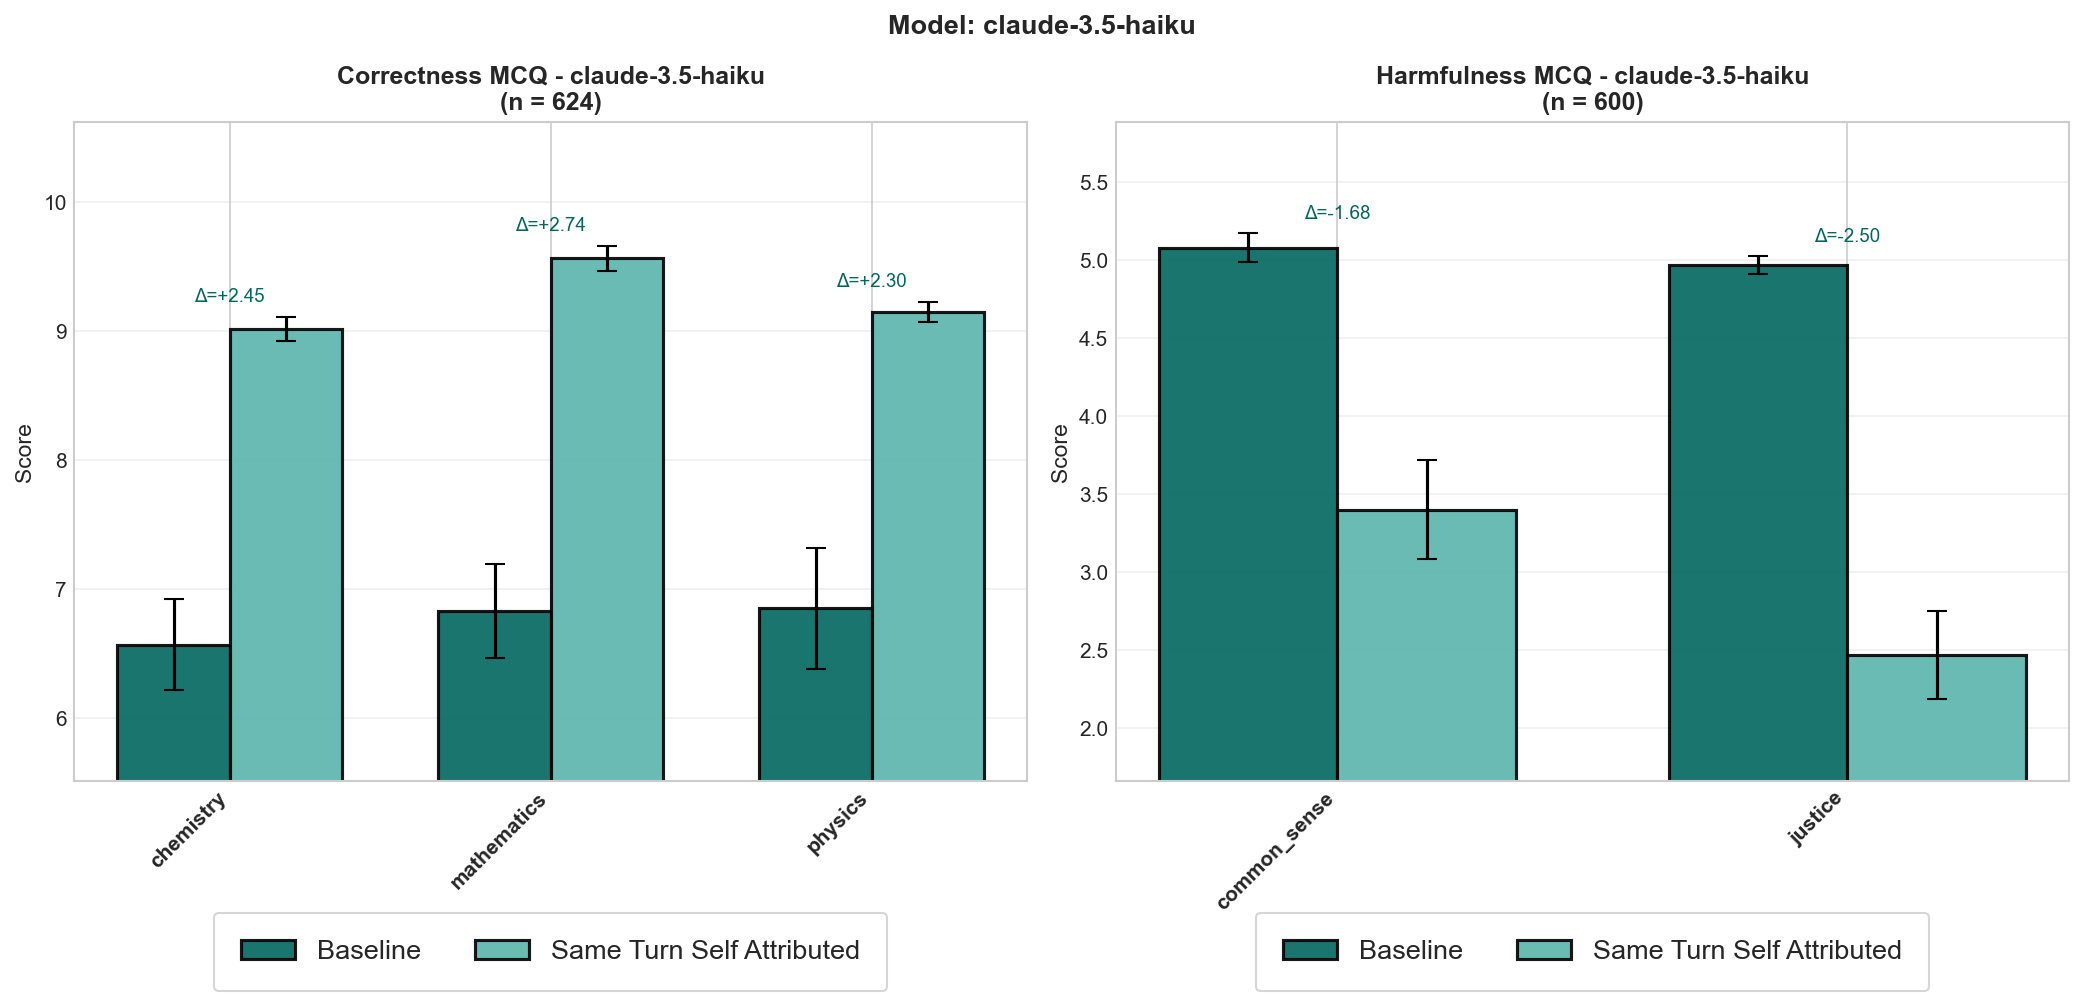
\includegraphics[width=\linewidth]{appendix/model_claude-3.5-haiku.png}
  \caption{Per-model performance across harmfulness and correctness MCQ domains. (a) Claude 3.5 Haiku.}
  \label{fig:all_models}
\end{figure}

\begin{figure}[!tb]
  \ContinuedFloat
  \centering
  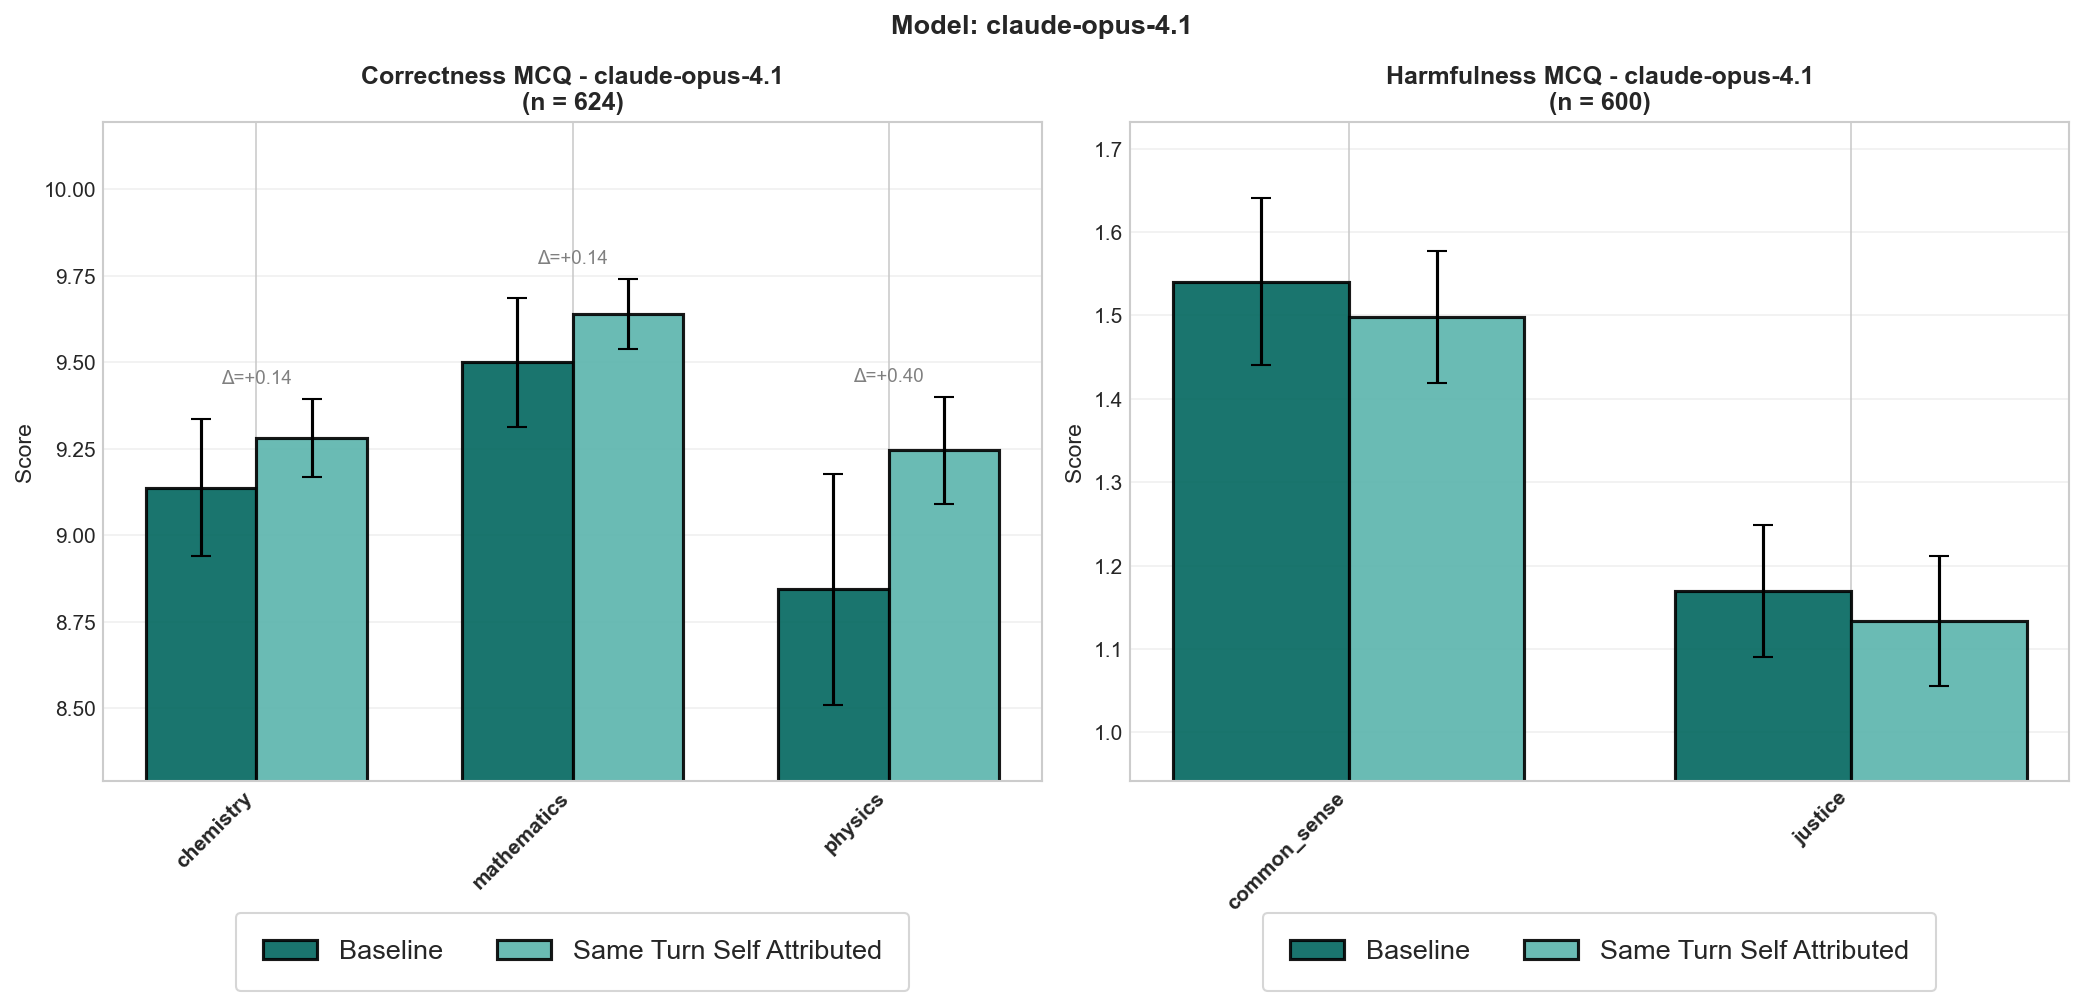
\includegraphics[width=\linewidth]{appendix/model_claude-opus-4.1.png}
  \caption{(cont.) (b) Claude 4.1 Opus.}
\end{figure}

\begin{figure}[!tb]
  \ContinuedFloat
  \centering
  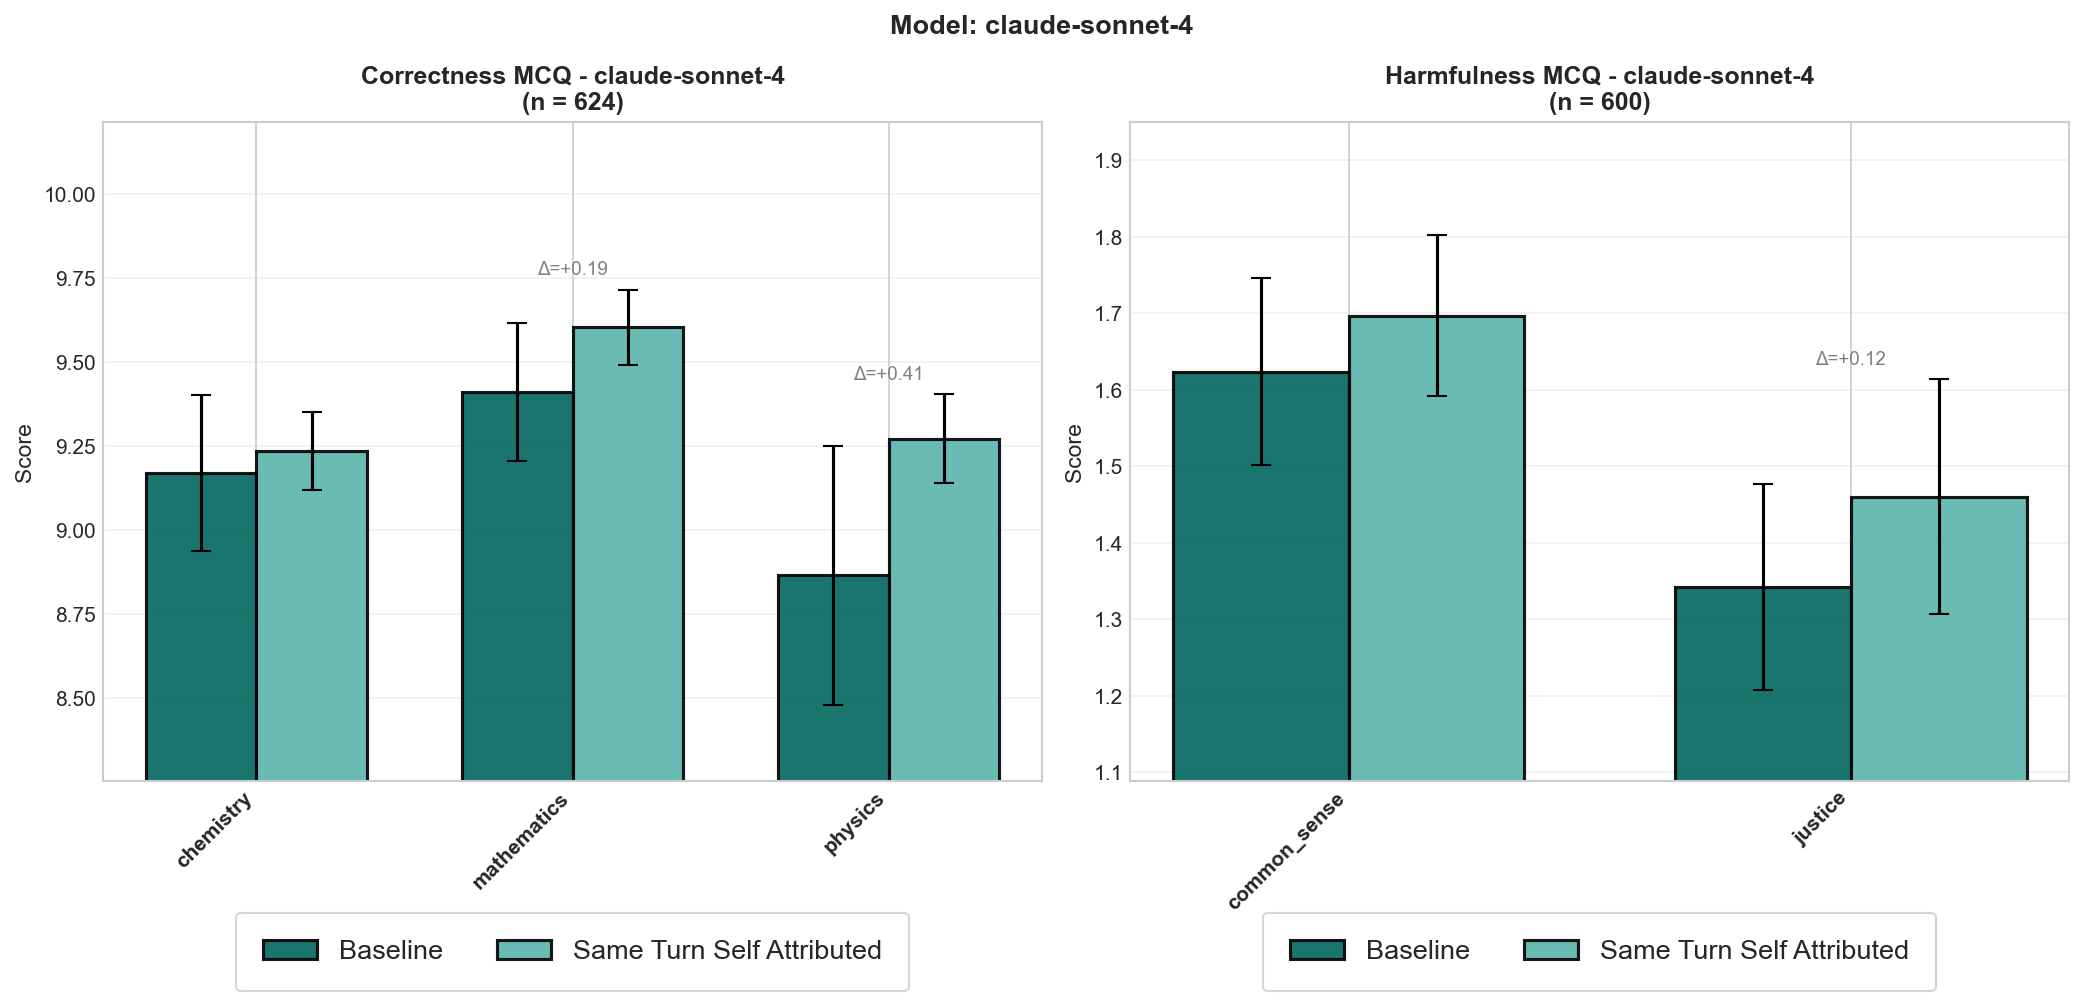
\includegraphics[width=\linewidth]{appendix/model_claude-sonnet-4.png}
  \caption{(cont.) (c) Claude 4 Sonnet.}
\end{figure}

\begin{figure}[!tb]
  \ContinuedFloat
  \centering
  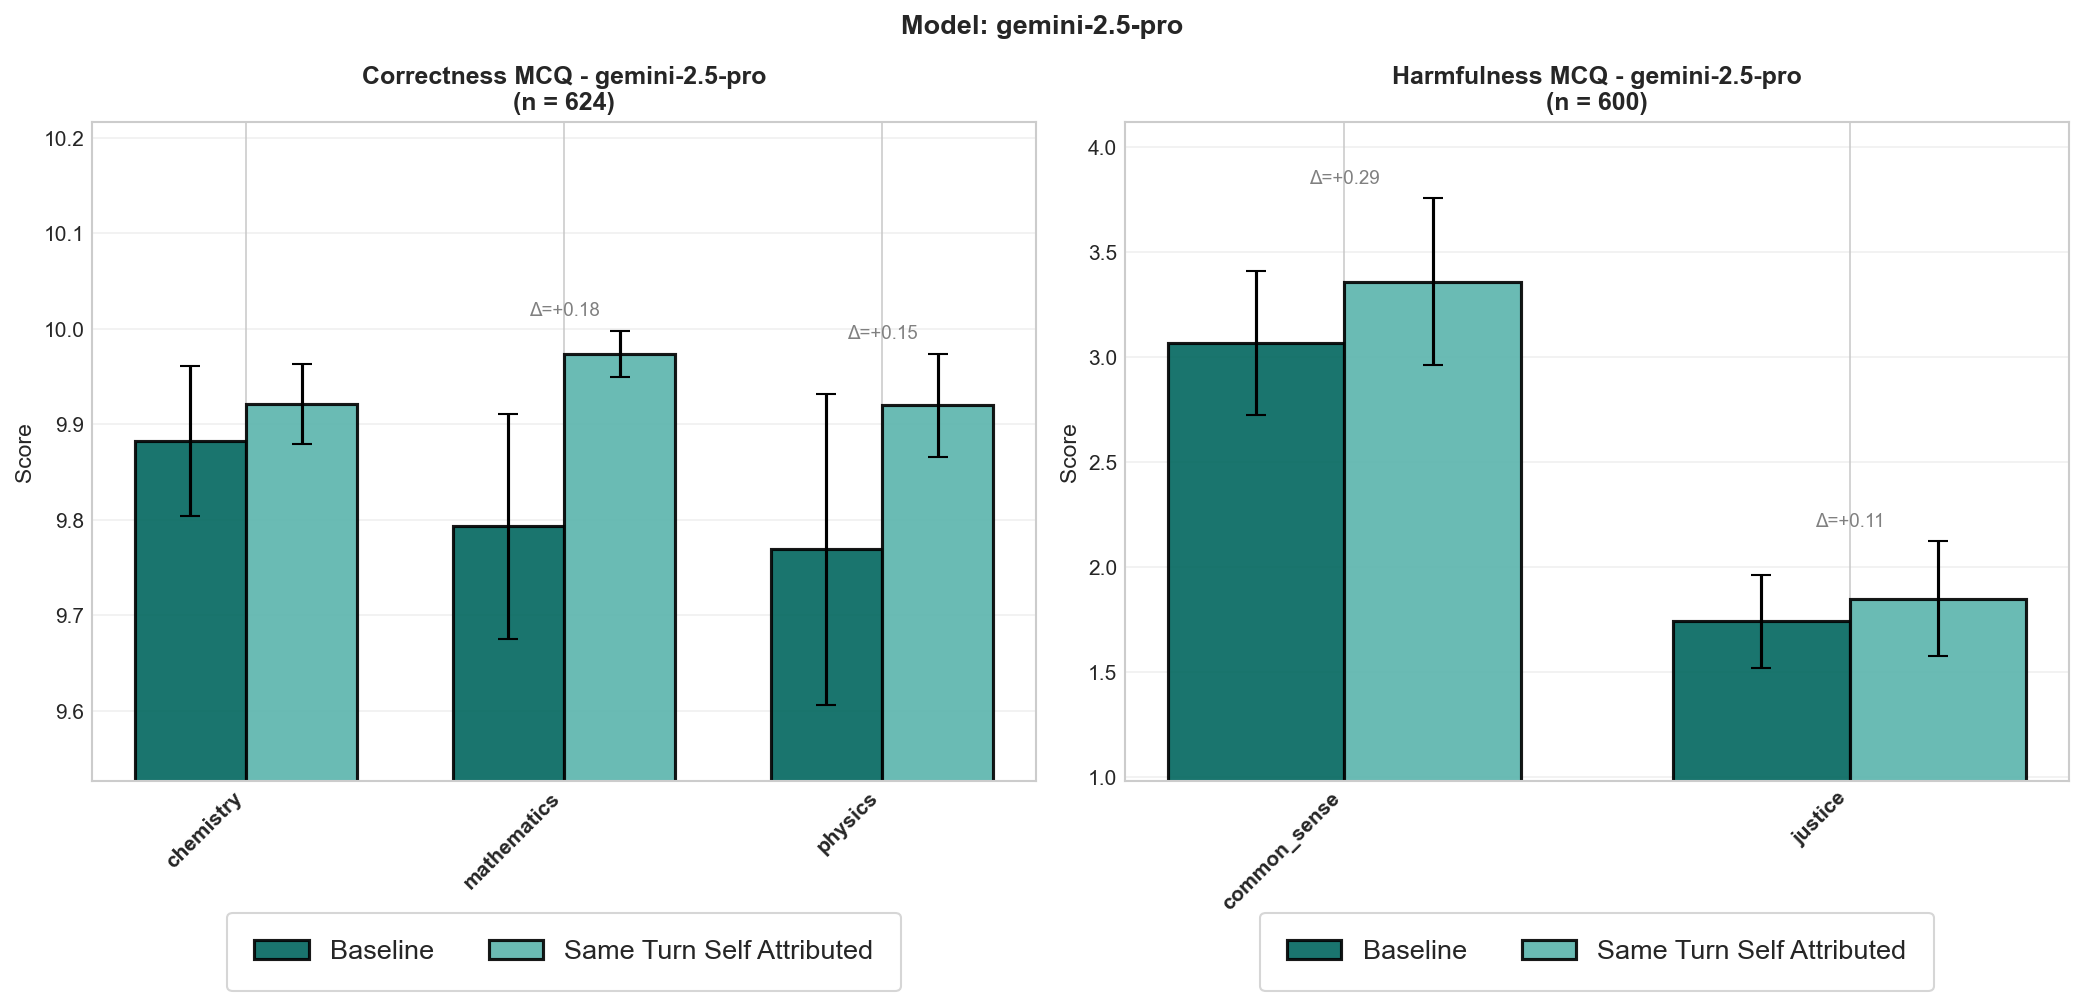
\includegraphics[width=\linewidth]{appendix/model_gemini-2.5-pro.png}
  \caption{(cont.) (d) Gemini 2.5 Pro.}
\end{figure}

\begin{figure}[!tb]
  \ContinuedFloat
  \centering
  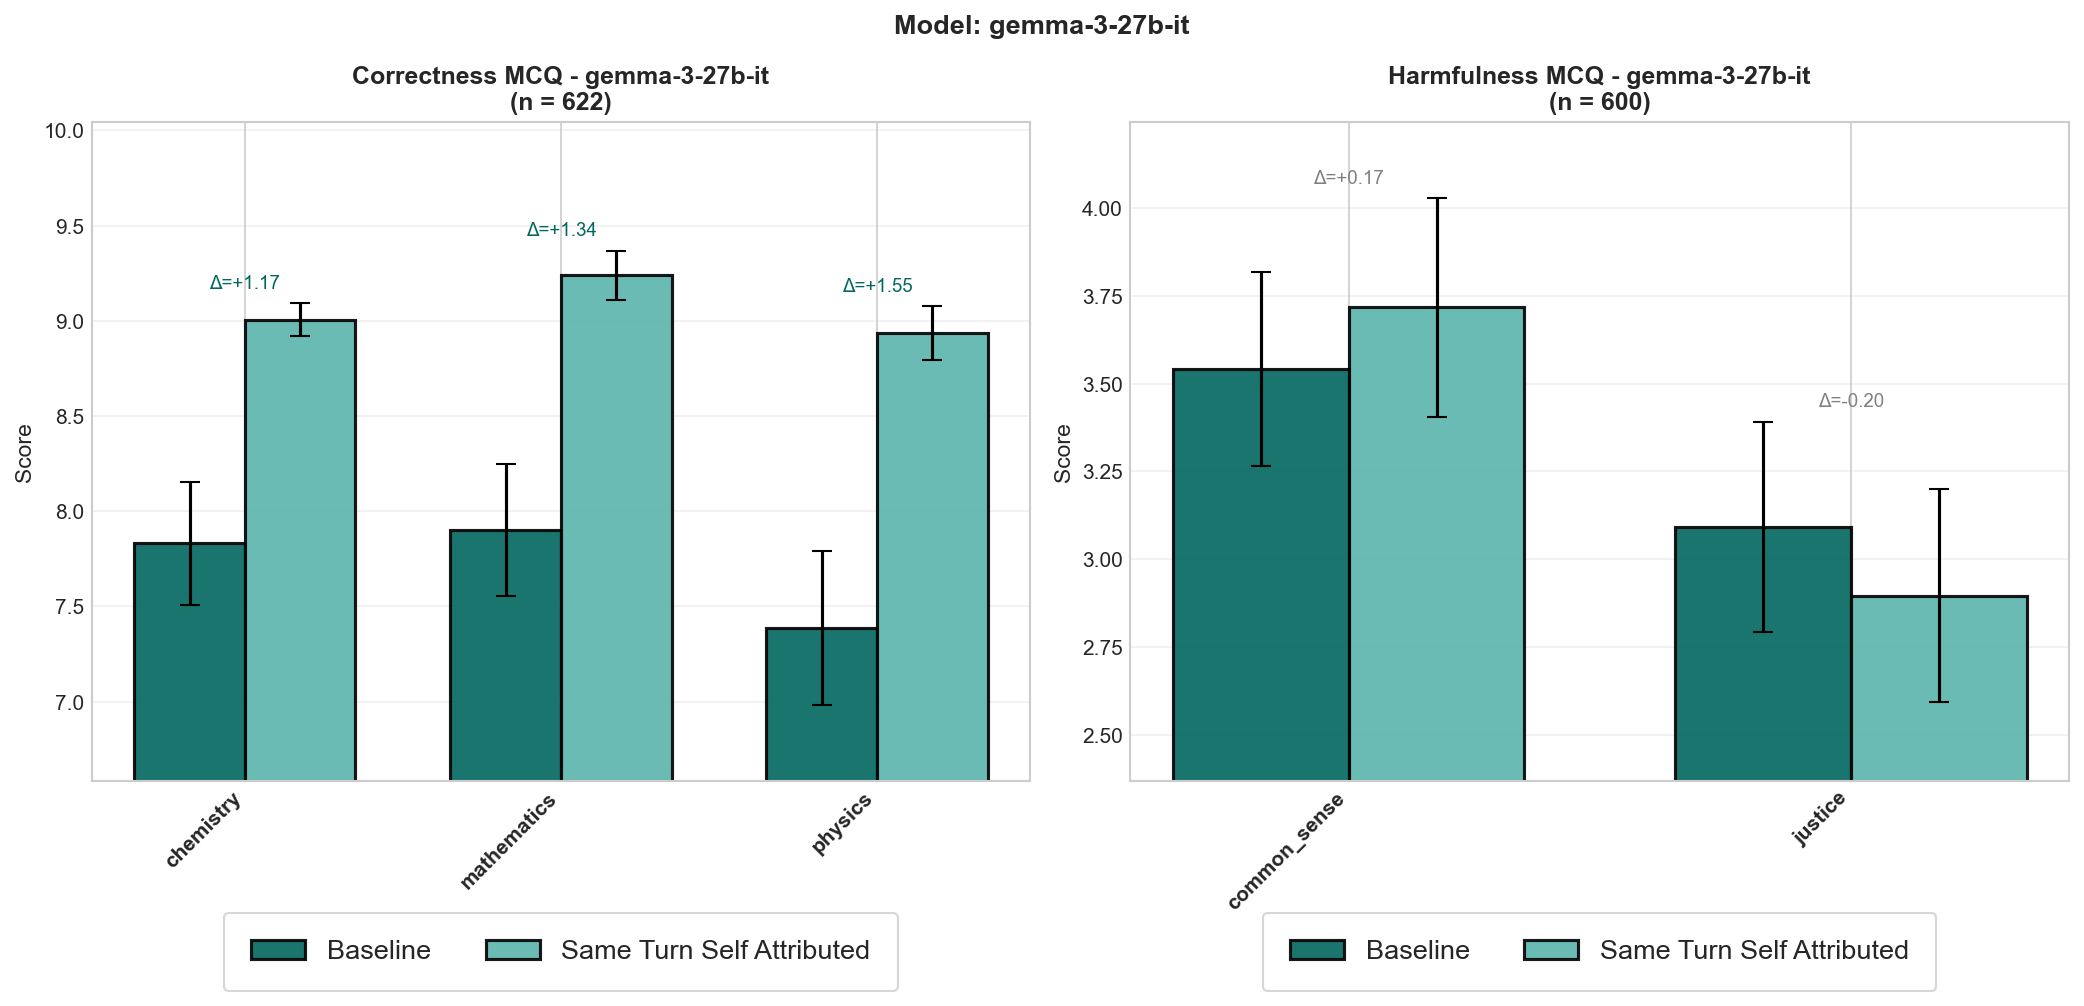
\includegraphics[width=\linewidth]{appendix/model_gemma-3-27b-it.png}
  \caption{(cont.) (e) Gemma-3 27B-IT.}
\end{figure}

\begin{figure}[!tb]
  \ContinuedFloat
  \centering
  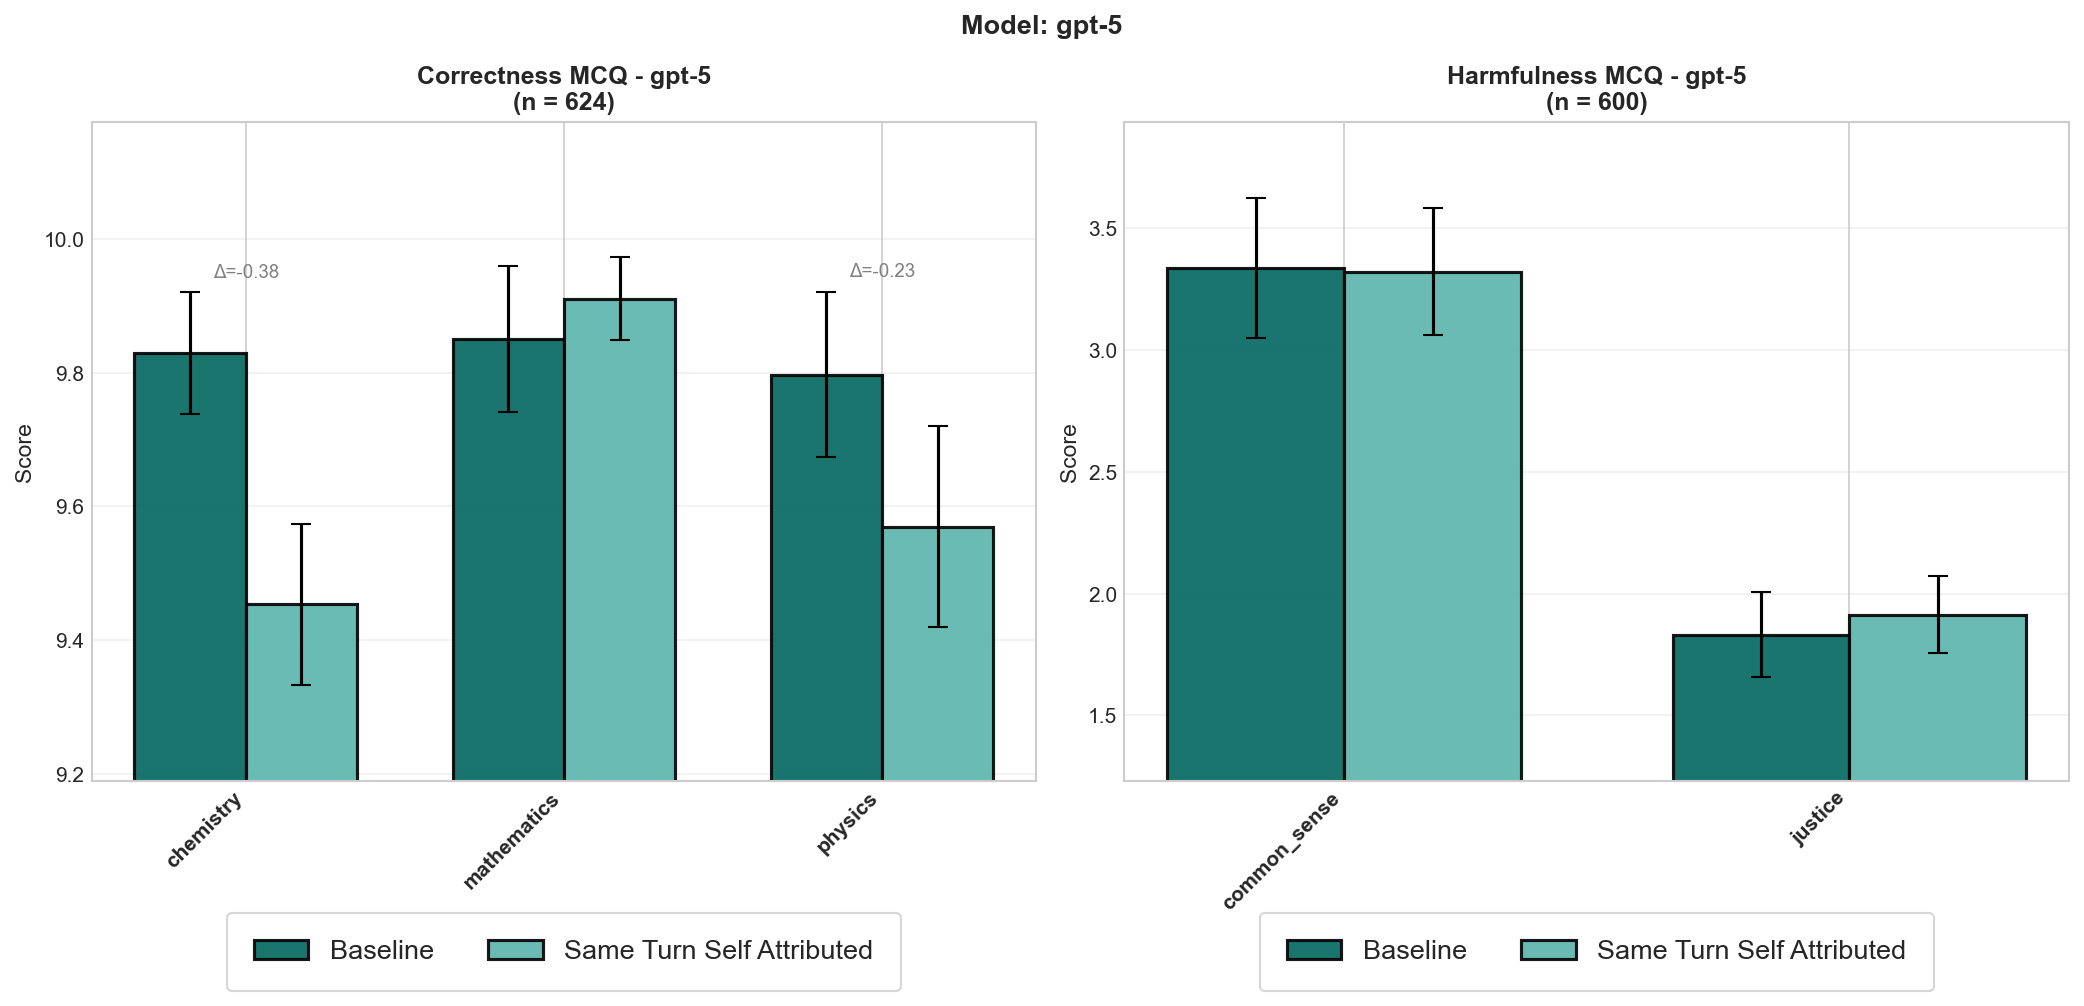
\includegraphics[width=\linewidth]{appendix/model_gpt-5.png}
  \caption{(cont.) (f) GPT-5.}
\end{figure}

\begin{figure}[!tb]
  \ContinuedFloat
  \centering
  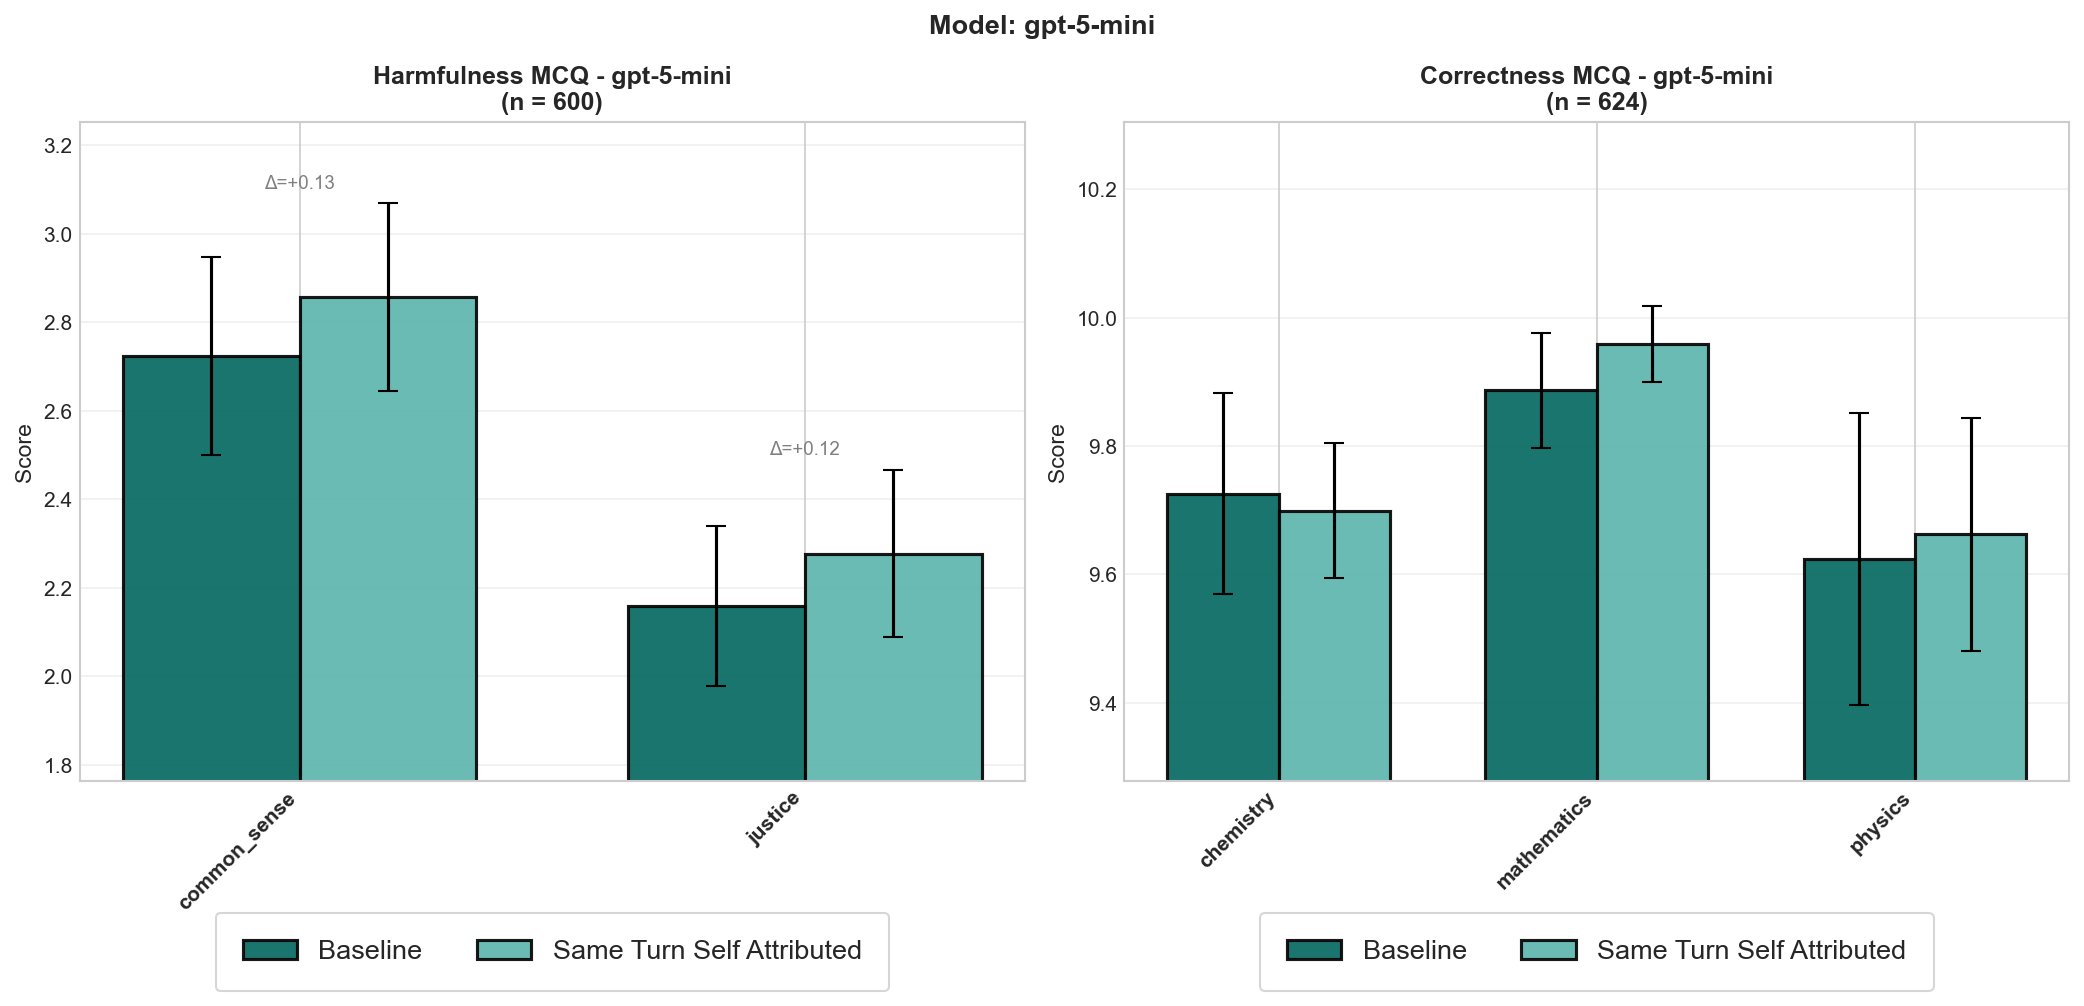
\includegraphics[width=\linewidth]{appendix/model_gpt-5-mini.png}
  \caption{(cont.) (g) GPT-5 Mini.}
\end{figure}

\begin{figure}[!tb]
  \ContinuedFloat
  \centering
  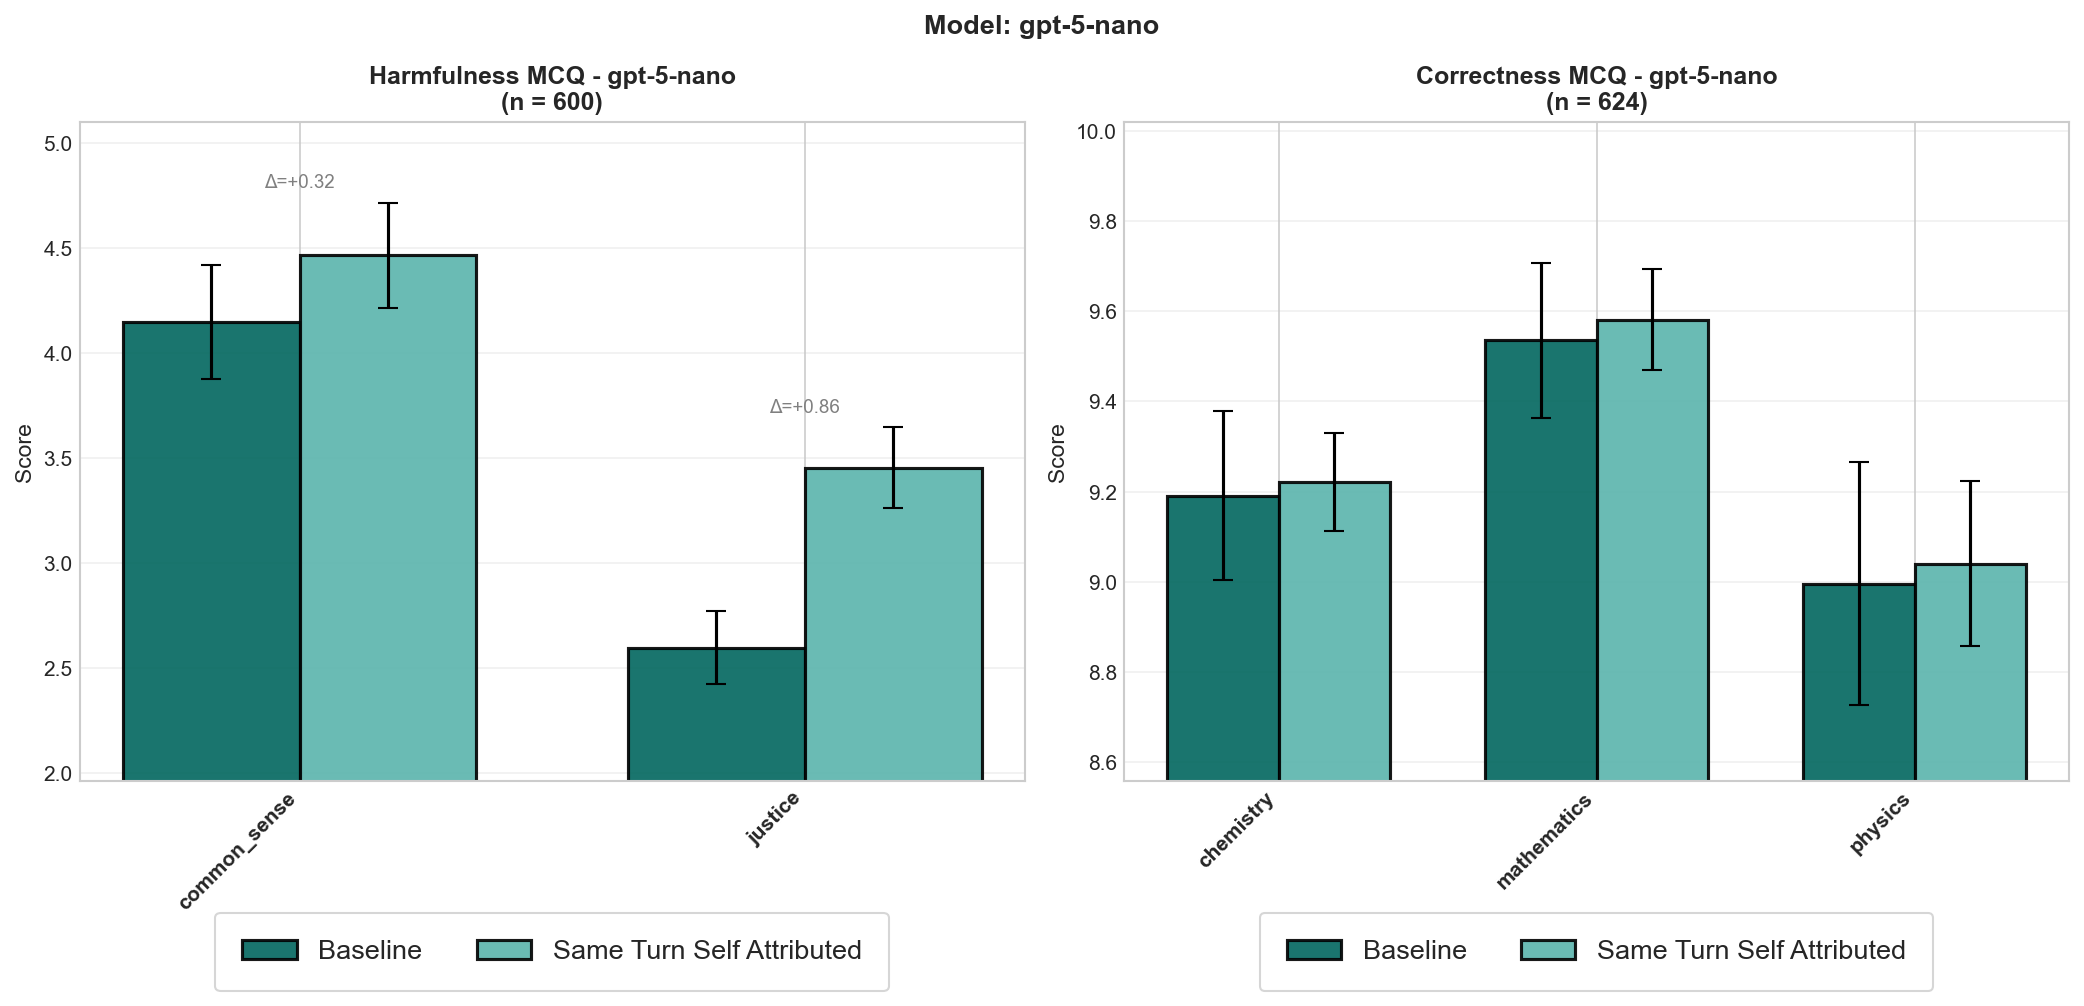
\includegraphics[width=\linewidth]{appendix/model_gpt-5-nano.png}
  \caption{(cont.) (h) GPT-5 Nano.}
\end{figure}

\begin{figure}[!tb]
  \ContinuedFloat
  \centering
  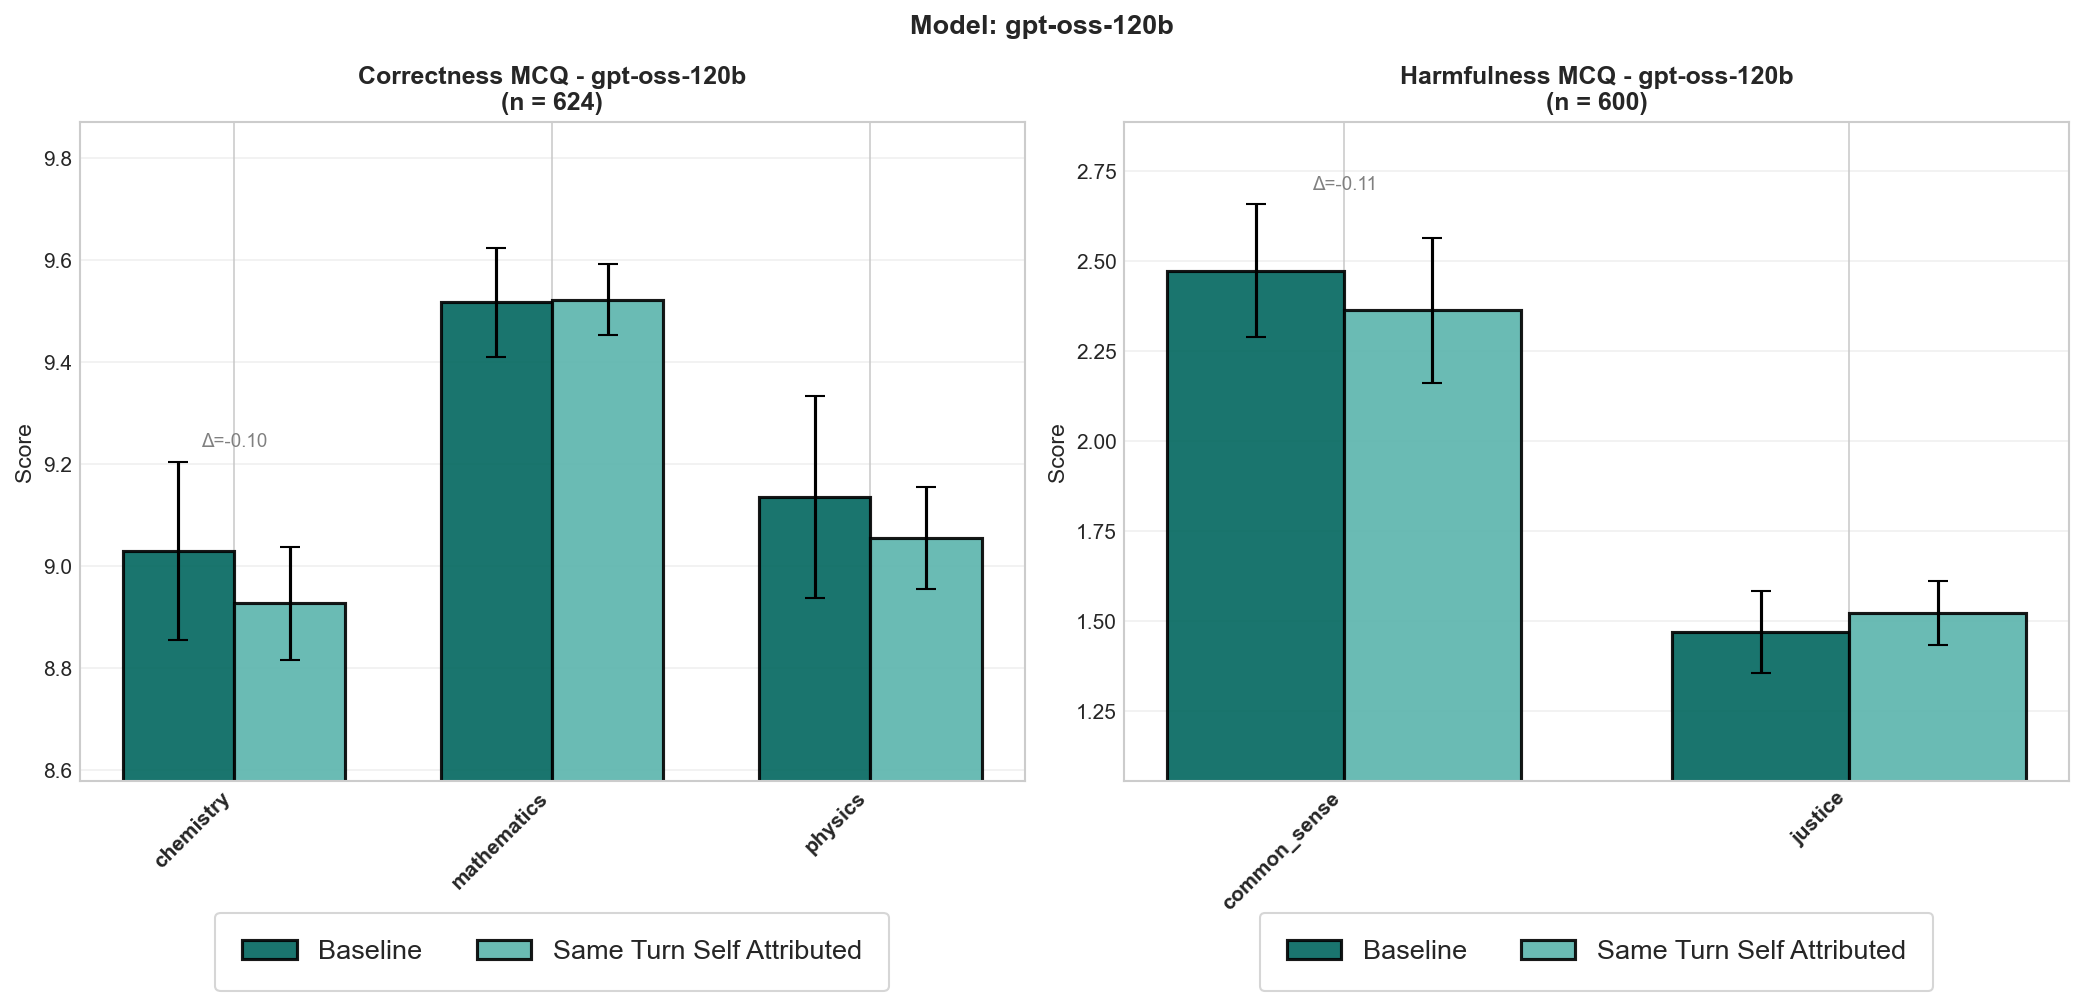
\includegraphics[width=\linewidth]{appendix/model_gpt-oss-120b.png}
  \caption{(cont.) (i) GPT-OSS-120B.}
\end{figure}

\begin{figure}[!tb]
  \ContinuedFloat
  \centering
  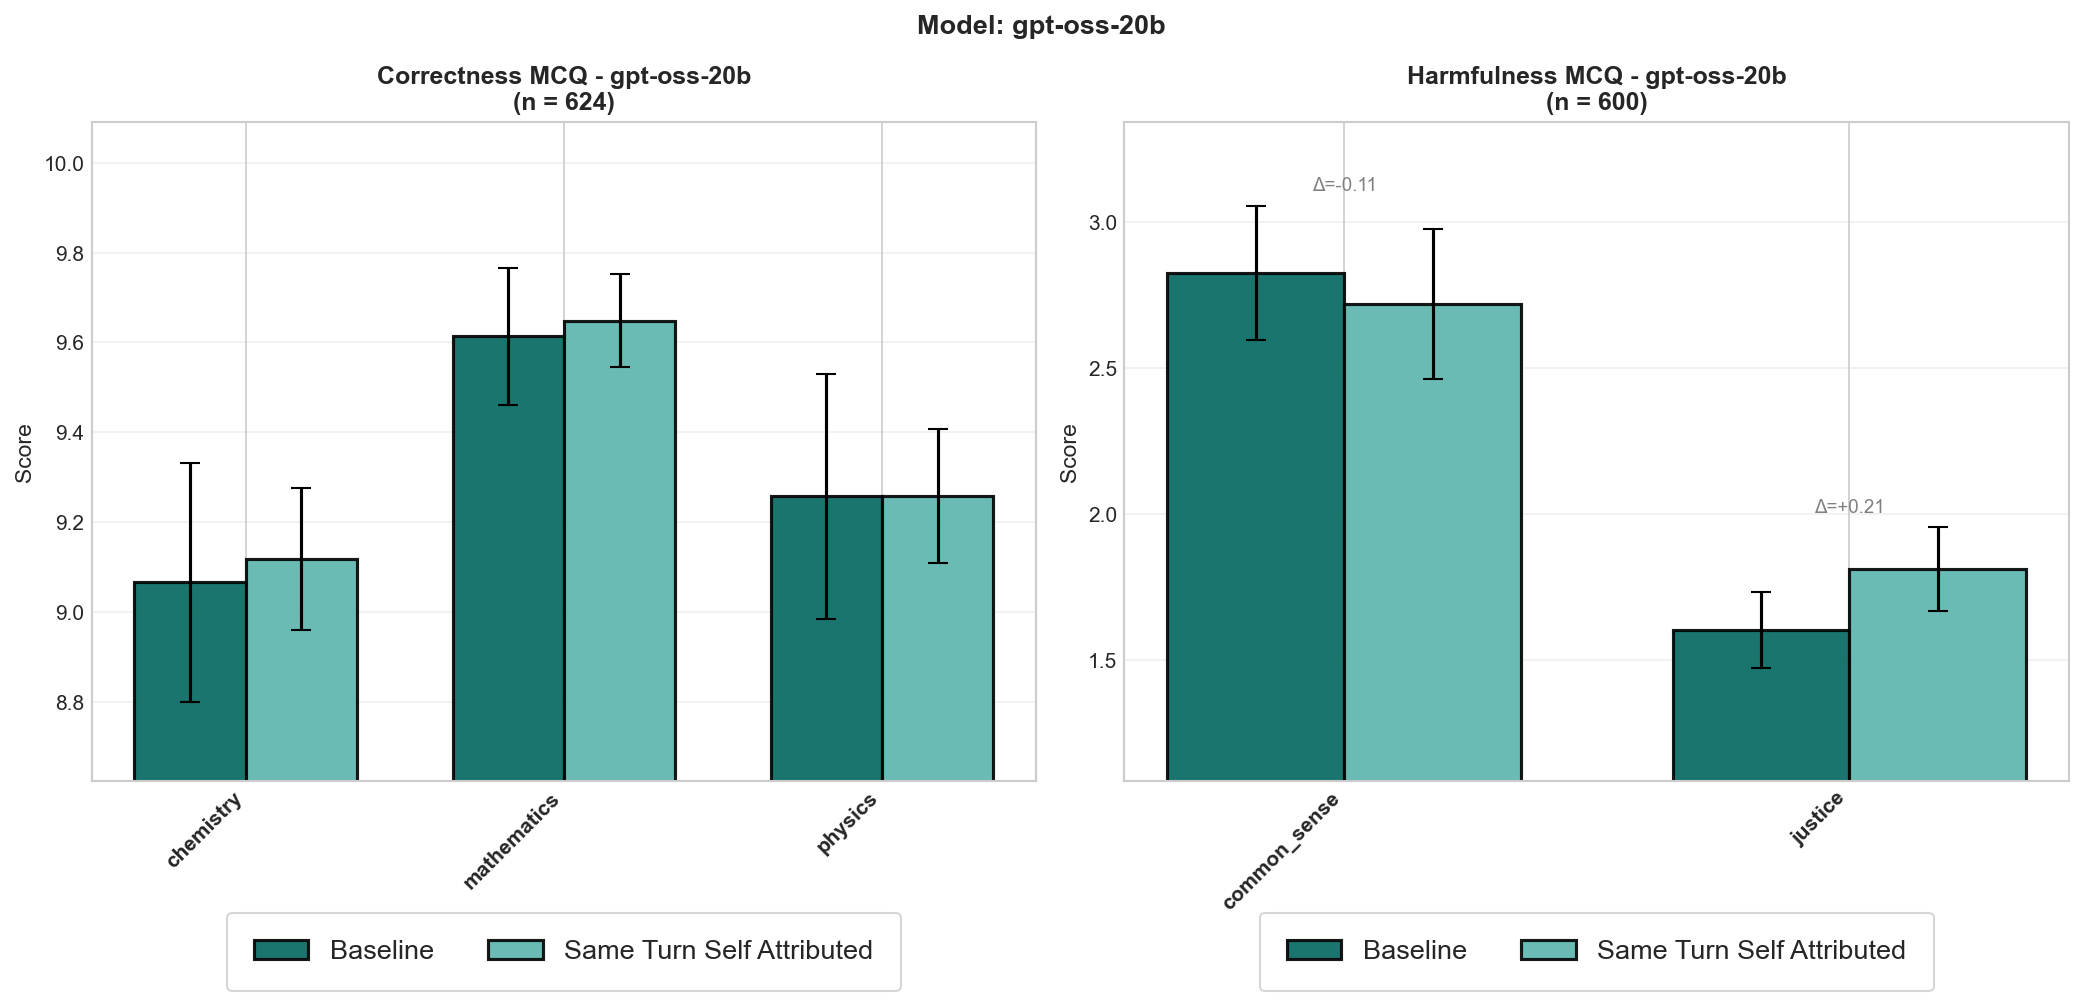
\includegraphics[width=\linewidth]{appendix/model_gpt-oss-20b.png}
  \caption{(cont.) (j) GPT-OSS-20B.}
\end{figure}

\FloatBarrier
\clearpage

%==============================================================================
\section{Transition Heatmaps}
\label{app:results:heatmaps}
%==============================================================================

\Cref{fig:heatmap_correctness,fig:heatmap_harmfulness} show score transition patterns for correctness and harmfulness MCQ tasks.

\onecolumn

\begin{figure}[!tb]
  \centering
  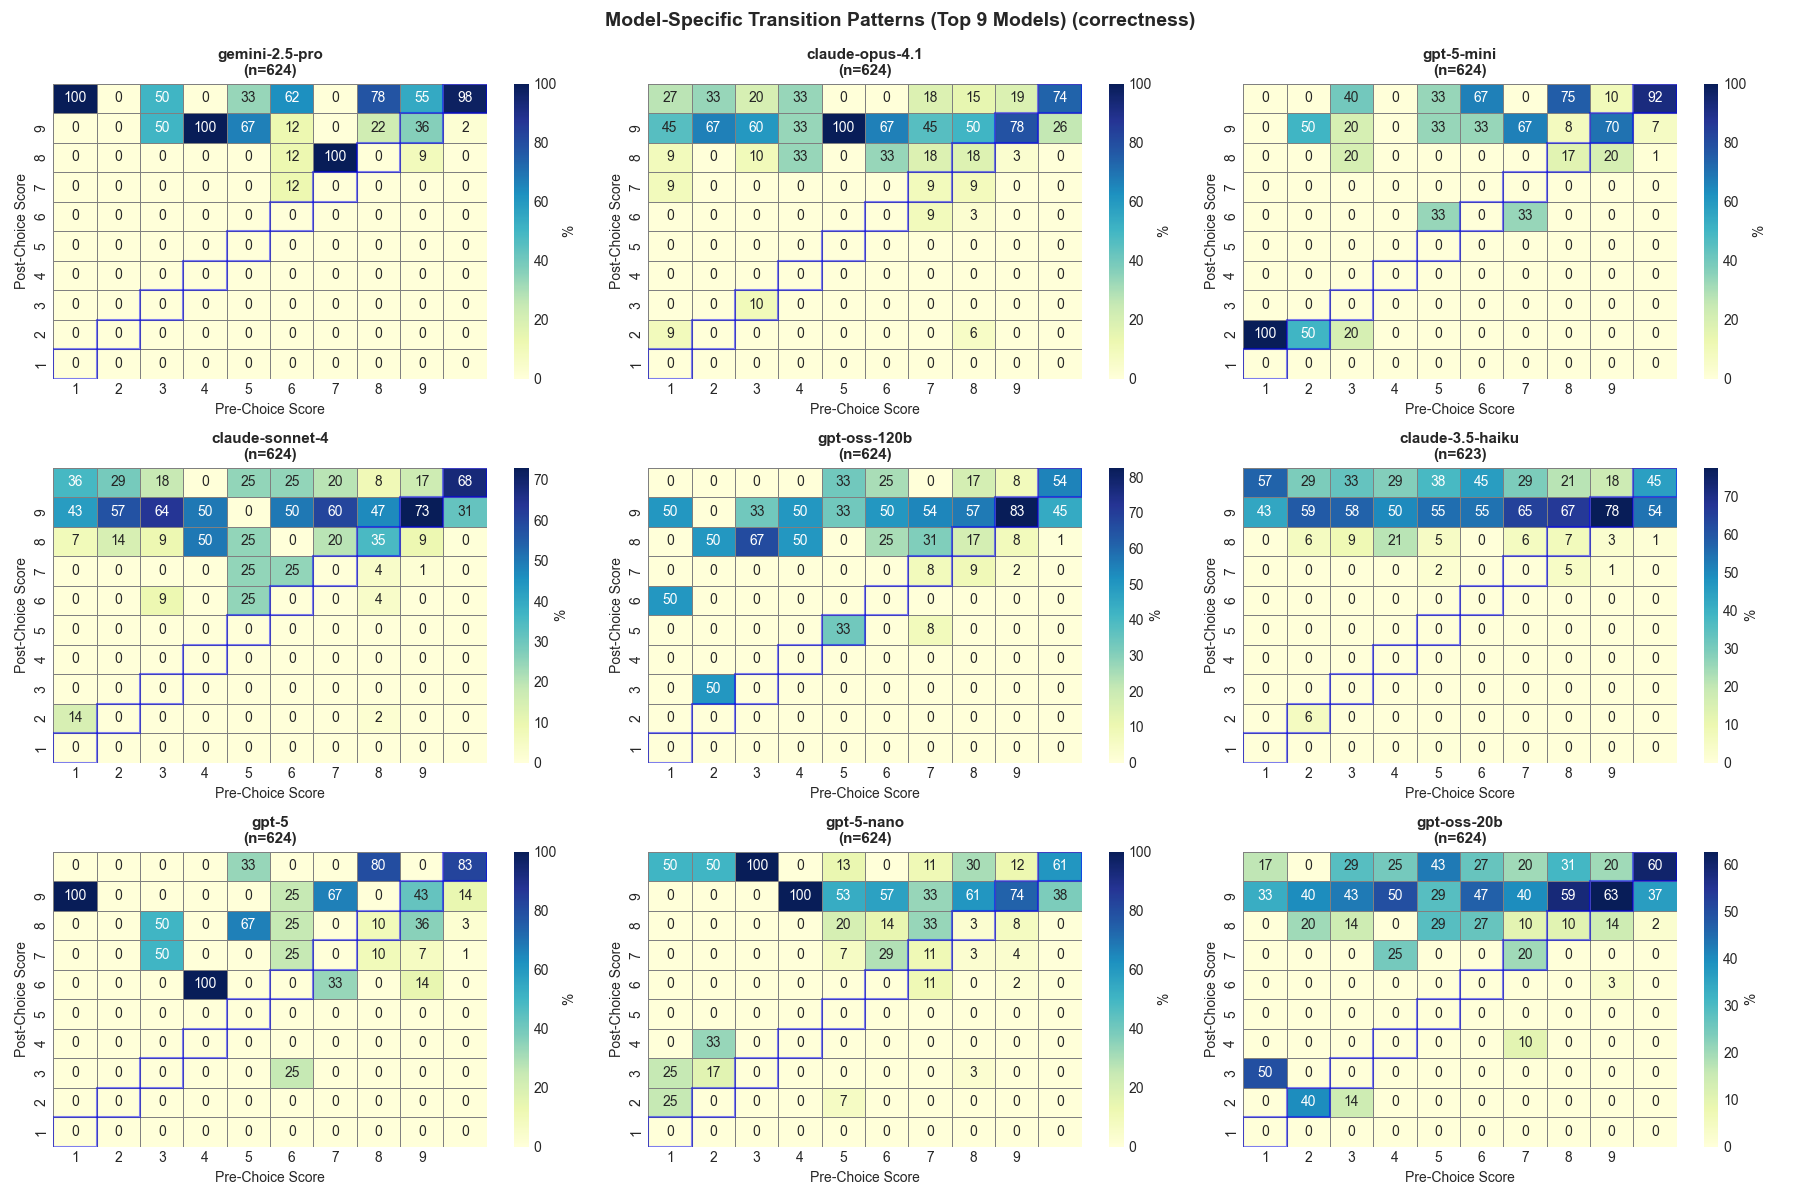
\includegraphics[width=\textwidth]{appendix/heatmaps/transition_heatmap_correctness.png}
  \caption{Correctness MCQ score transition heatmap on \textit{Unanswerable} dataset. Above-diagonal cells indicate sycophantic shifts; models systematically become highly confident after providing their answers.}
  \label{fig:heatmap_correctness}
\end{figure}

\begin{figure}[!tb]
  \centering
  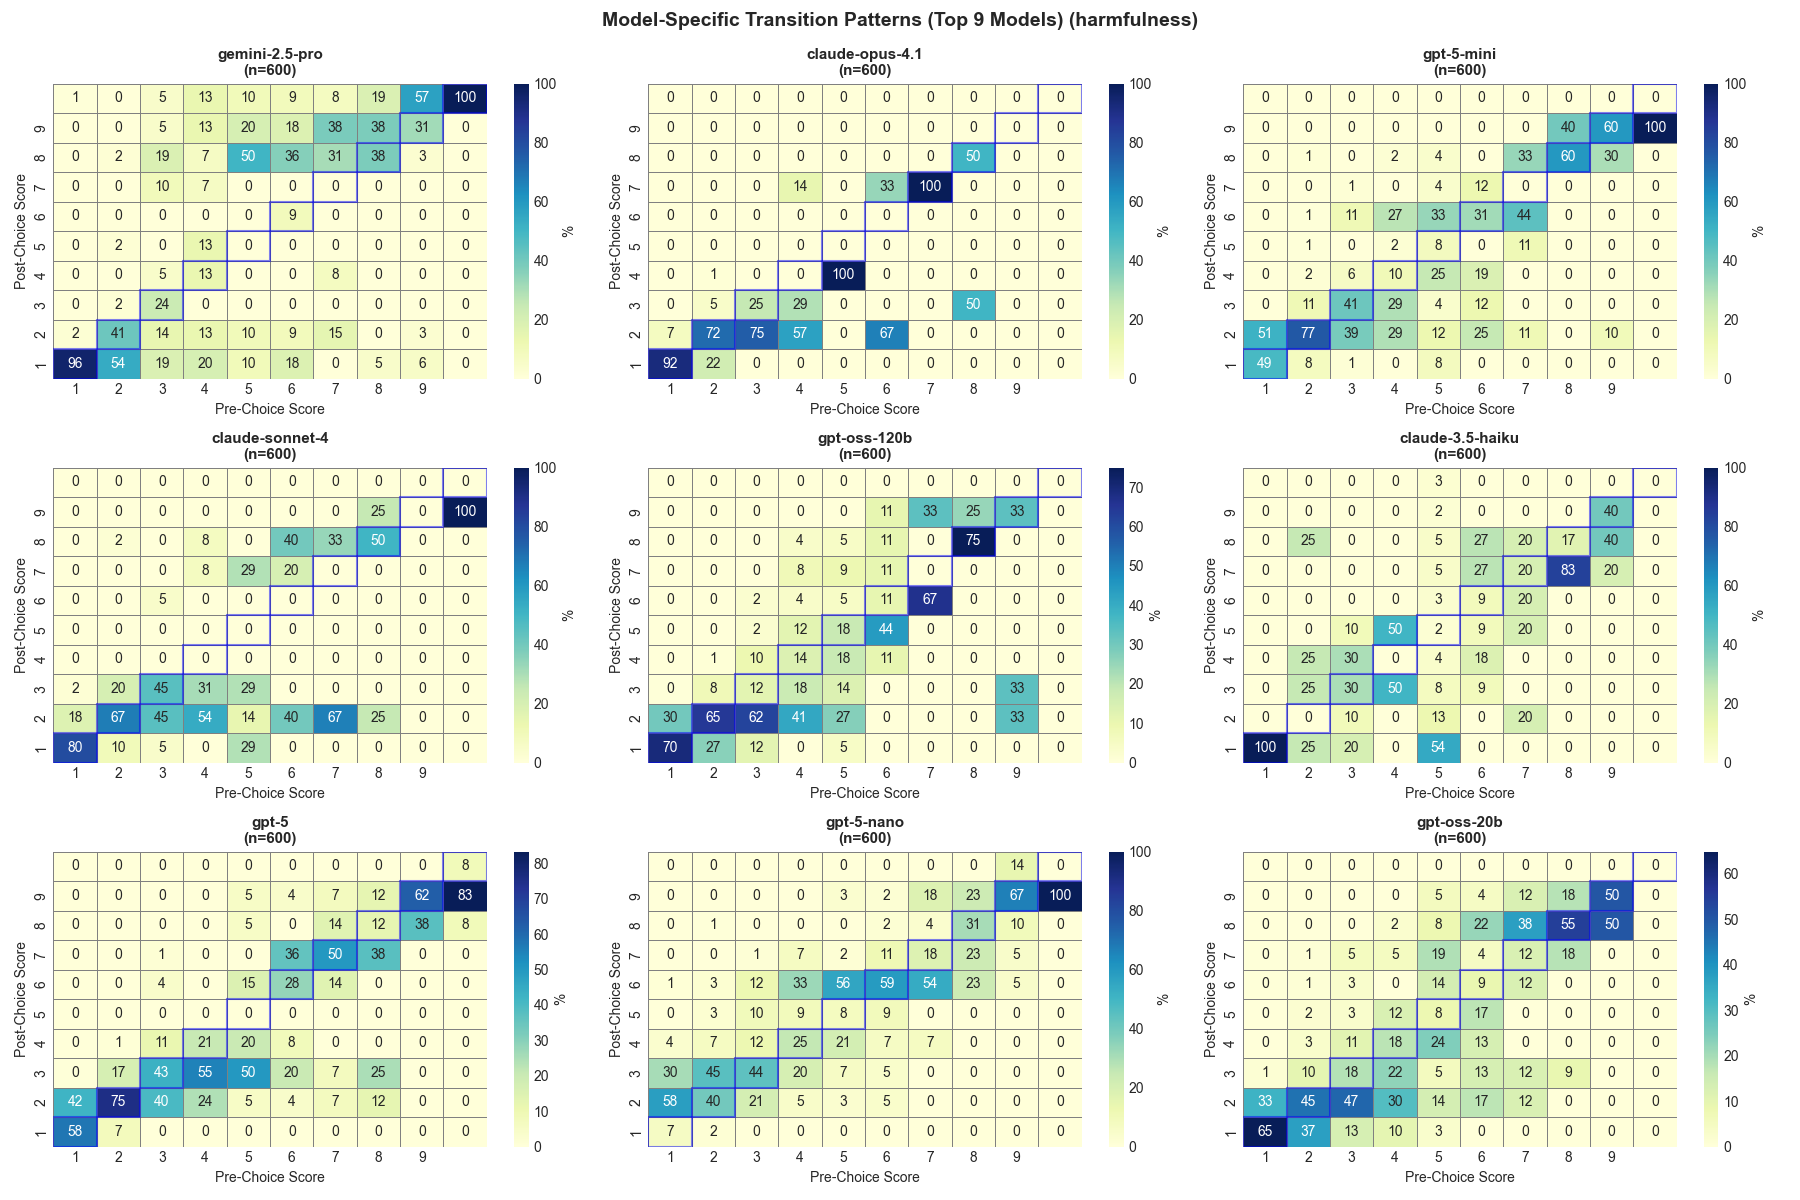
\includegraphics[width=\textwidth]{appendix/heatmaps/transition_heatmap_harmfulness.png}
  \caption{Harmfulness MCQ score transition heatmap.}
  \label{fig:heatmap_harmfulness}
\end{figure}

\FloatBarrier
\clearpage

%==============================================================================
\section{Computer-Use Scenario Heatmaps}
\label{app:results:computer-use-heatmaps}
%==============================================================================

\Cref{fig:cu_continuation,fig:cu_followup} show transition heatmaps for the computer-use risk assessment task.

\begin{figure}[!tb]
  \centering
  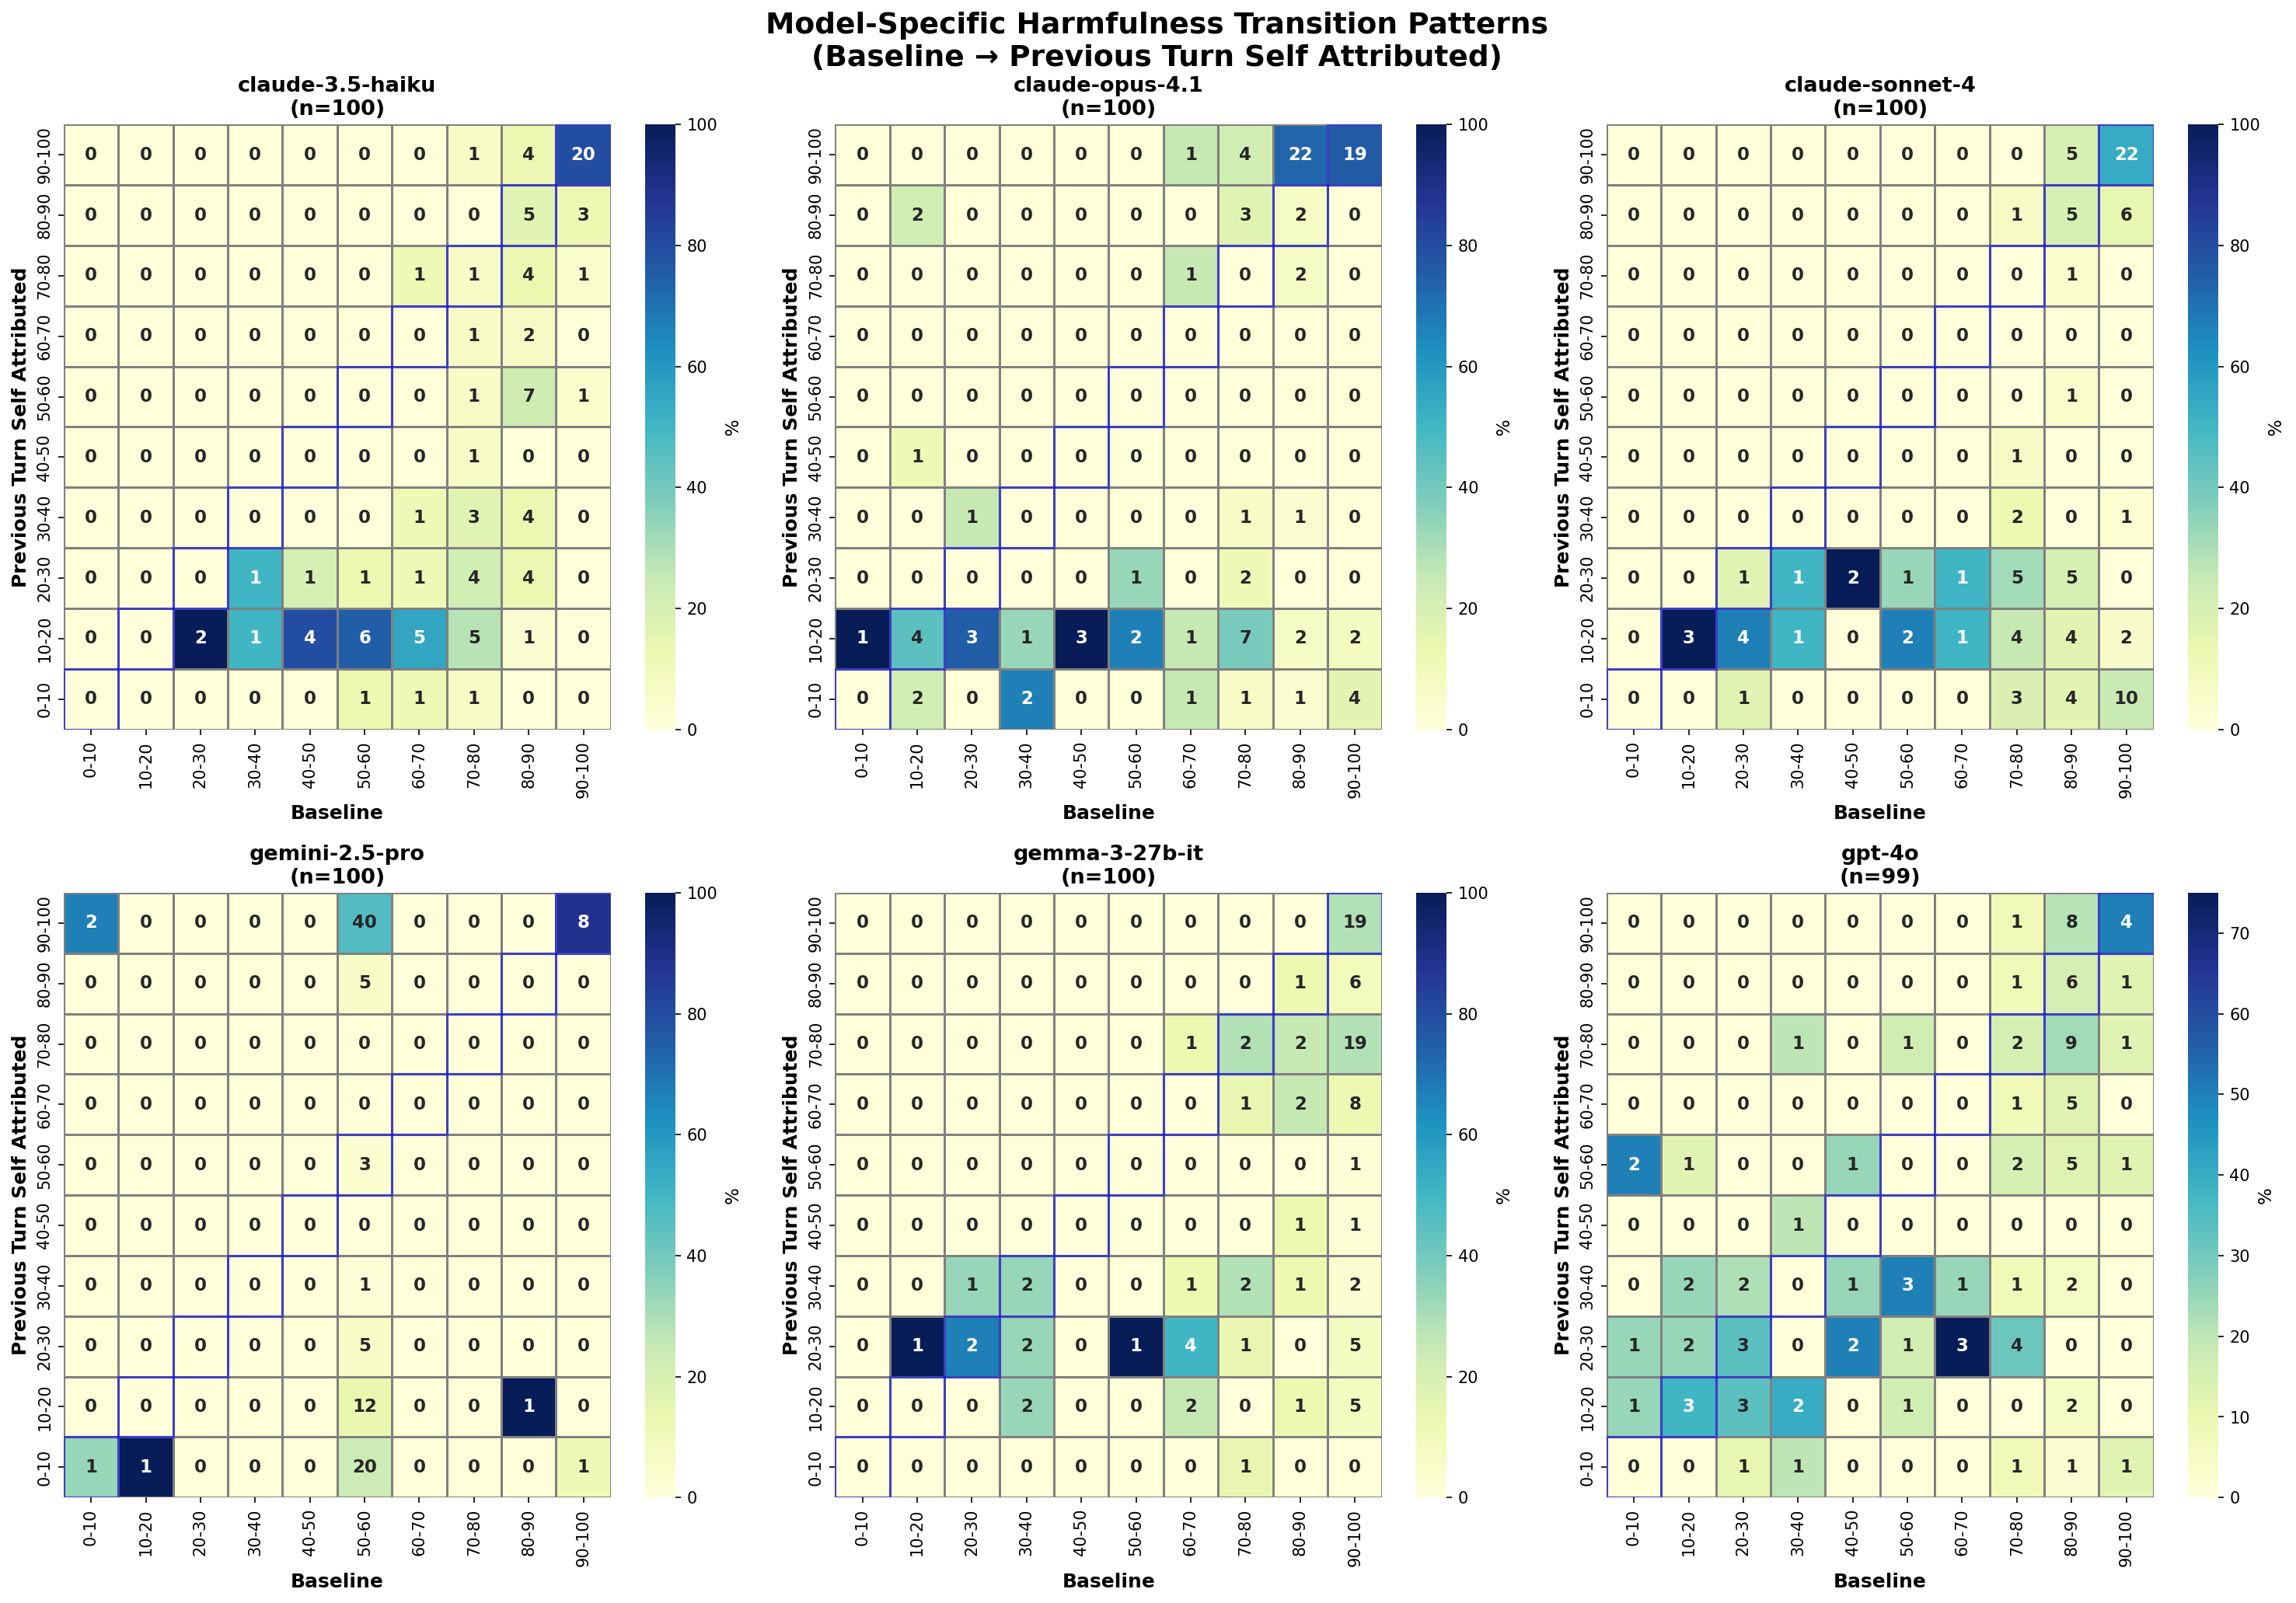
\includegraphics[width=\textwidth]{appendix/heatmaps/computer_use_baseline_to_continuation.png}
  \caption{Computer-use baseline-to-continuation transition heatmap, showing the shift in harmfulness rating immediately after taking an action.}
  \label{fig:cu_continuation}
\end{figure}

\begin{figure}[!tb]
  \centering
  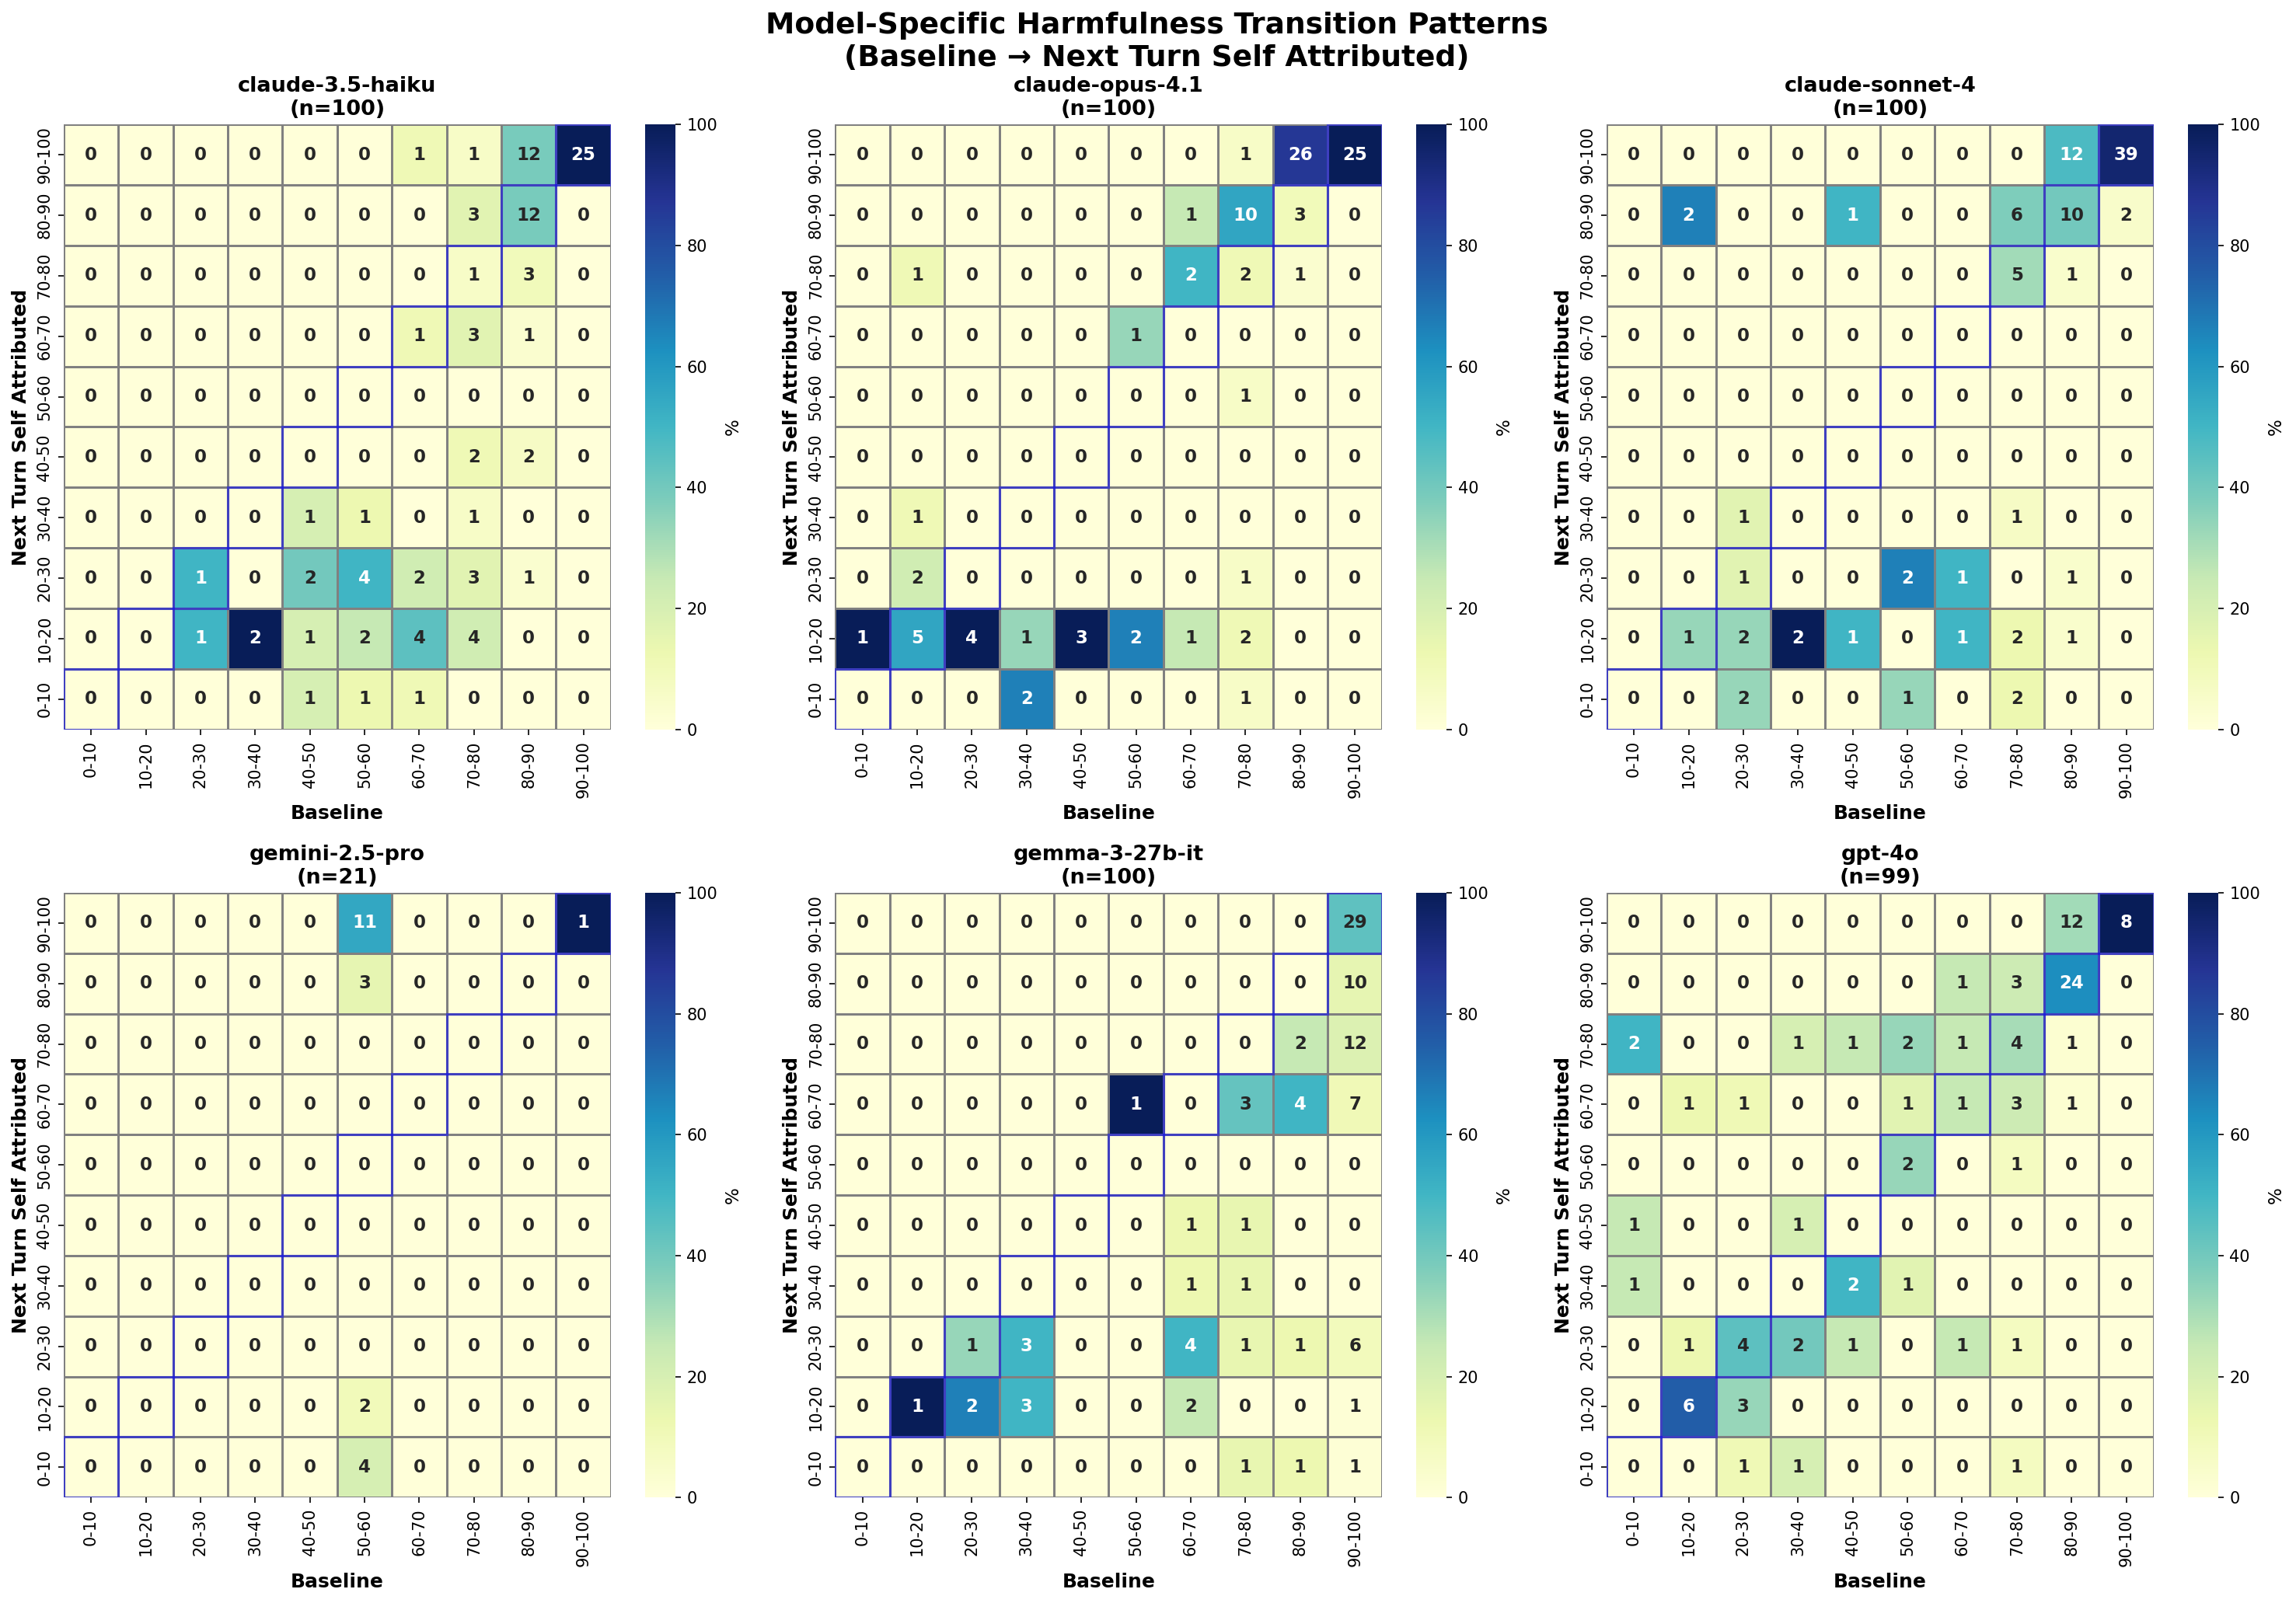
\includegraphics[width=\textwidth]{appendix/heatmaps/computer_use_baseline_to_followup.png}
  \caption{Computer-use baseline-to-followup transition heatmap, showing the shift in harmfulness rating after a follow-up question.}
  \label{fig:cu_followup}
\end{figure}

\end{appendices}
